\documentclass[a4paper,11pt]{article}
\usepackage{amsmath}
\usepackage{amsthm}
\usepackage{amsfonts}
\usepackage{mathrsfs}
\usepackage{amssymb}
\usepackage{mathpazo}
\usepackage[dvipsnames]{xcolor}
\usepackage{bm}
\usepackage[no-weekday]{eukdate}
\usepackage[bb=boondox]{mathalfa}
\usepackage{paralist}
\usepackage{natbib}
\usepackage{url}
\usepackage[textwidth=6.1in,textheight = 10in]{geometry}
\usepackage{placeins}
\usepackage[hidelinks]{hyperref}
\usepackage{multirow, float}
\usepackage{makecell}
\usepackage{calc}
\usepackage{graphicx}
\usepackage{enumitem}

\setlength{\parskip}{0cm}
\setlength{\parindent}{1em}
\usepackage[compact]{titlesec}
\titlespacing{\section}{0pt}{2ex}{1ex}
\titlespacing{\subsection}{0pt}{1ex}{0ex}
\titlespacing{\subsubsection}{0pt}{0.5ex}{0ex}
\usepackage{titling}\pretitle{\begin{center}\LARGE\bfseries}
\usepackage[bottom,hang,flushmargin]{footmisc}
\usepackage{adjustbox}

%% LINE AND PAGE BREAKING
\sloppy
\allowdisplaybreaks
\clubpenalty = 10000
\widowpenalty = 10000
\brokenpenalty = 10000
\RequirePackage{microtype}

% NOTE: To produce blinded version, replace "0" with "1" below.
\newcommand{\blind}{1}

%\usepackage{setspace}
\usepackage{caption}
\captionsetup[figure]{labelfont={bf}, font = small, singlelinecheck=true}
\captionsetup[table]{labelfont={bf}, font = small, singlelinecheck=true}
\usepackage{subcaption}

\DeclareMathOperator*{\argmin}{arg\,min}
\usepackage{longtable}
\usepackage{booktabs}
\usepackage{array}
\newcolumntype{M}[1]{>{\centering\arraybackslash}m{#1}}
\newcolumntype{L}[1]{>{\raggedright\arraybackslash}m{#1}}
\newcolumntype{R}[1]{>{\raggedleft\arraybackslash}m{#1}}

\newcommand{\alphavet}{\bm{\alpha}}
\newcommand{\betavet}{\bm{\beta}}
\newcommand{\epsvet}{\bm{\varepsilon}}
\newcommand{\etavet}{\bm{\eta}}
\newcommand{\lambdavet}{\bm{\lambda}}
\newcommand{\Unovet}{\bm{1}}
\newcommand{\avet}{\bm{a}}
\newcommand{\bvet}{\bm{b}}
\newcommand{\cvet}{\bm{c}}
\newcommand{\dvet}{\bm{d}}
\newcommand{\evet}{\bm{e}}
\newcommand{\pvet}{\bm{p}}
\newcommand{\fvet}{\bm{f}}
\newcommand{\tvet}{\bm{t}}
\newcommand{\uvet}{\bm{u}}
\newcommand{\vvet}{\bm{v}}
\newcommand{\wvet}{\bm{w}}
\newcommand{\xvet}{\bm{x}}
\newcommand{\yvet}{\bm{y}}
\newcommand{\zvet}{\bm{z}}
\newcommand{\Avet}{\bm{A}}
\newcommand{\Bvet}{\bm{B}}
\newcommand{\Cvet}{\bm{C}}
\newcommand{\Dvet}{\bm{D}}
\newcommand{\Evet}{\bm{E}}
\newcommand{\Fvet}{\bm{F}}
\newcommand{\Gvet}{\bm{G}}
\newcommand{\Hvet}{\bm{H}}
\newcommand{\Ivet}{\bm{I}}
\newcommand{\Jvet}{\bm{J}}
\newcommand{\Kvet}{\bm{K}}
\newcommand{\Lvet}{\bm{L}}
\newcommand{\Mvet}{\bm{M}}
\newcommand{\Nvet}{\bm{N}}
\newcommand{\Pvet}{\bm{P}}
\newcommand{\Qvet}{\bm{Q}}
\newcommand{\Rvet}{\bm{R}}
\newcommand{\Svet}{\bm{S}}
\newcommand{\Tvet}{\bm{T}}
\newcommand{\Uvet}{\bm{U}}
\newcommand{\Wvet}{\bm{W}}
\newcommand{\Xvet}{\bm{X}}
\newcommand{\Yvet}{\bm{Y}}
\newcommand{\Zvet}{\bm{Z}}
\newcommand{\Zerovet}{\bm{0}}
\newcommand{\Omegavet}{\bm{\Omega}}
\newcommand{\Sigmavet}{\bm{\Sigma}}

\definecolor{mybluehl}{HTML}{cbd3ff}

% theorem
\makeatletter
\def\@endtheorem{\endtrivlist}
\makeatother

%% tikz
%% Packages to draw hierarchies
\usepackage{tikz}
\usepackage{forest}

\usetikzlibrary{arrows,shapes,positioning,shadows,trees}
\usetikzlibrary{matrix, decorations.pathreplacing, arrows, calc, fit, arrows.meta, decorations.pathmorphing, decorations.markings}

\tikzset{
  basic/.style  = {draw, text width=2cm, drop shadow, font=\sffamily, rectangle},
  root/.style   = {basic, rounded corners=2pt, thin, align=center,
                   fill=green!30},
  level 2/.style = {basic, rounded corners=6pt, thin,align=center, fill=green!60,
                   text width=4em},
  level 3/.style = {basic, thin, align=left, fill=pink!60, text width=1.5em}
}
\newcommand{\relation}[3]
{
	\draw (#3.south) -- +(0,-#1) -| ($ (#2.north) $)
}
\newcommand{\relationW}[2]
{
	\draw (#2.west) -| ($ (#1.north) $)
}
\newcommand{\relationE}[2]
{
	\draw (#2.east) -| ($ (#1.north) $)
}

\newcommand{\relationD}[3]
{
	\draw (#3.east) -- +(#1,0) |- (#2.west)
}

\pgfdeclareimage[height=0.85cm]{ngreen}{fig/boot/ngreen.pdf}
\pgfdeclareimage[height=0.85cm]{nblue}{fig/boot/nblue.pdf}
\pgfdeclareimage[height=0.85cm]{nred}{fig/boot/nred.pdf}
\pgfdeclareimage[height=0.85cm]{nblack}{fig/boot/nblack.pdf}

\theoremstyle{definition}
\newtheorem{definition}{Definition}[section]
\newtheorem{theorem}{Theorem}[section]

% Title page
\makeatletter
\newcommand{\maketitleblind}{\begingroup%
\if1\blind
{
\clearpage\maketitle
\thispagestyle{empty}
\vfill
%\vskip2cm
%\noindent\textit{\large\textbf{Preliminary Working Draft}}\\
%\noindent\textbf{Please do not quote or cite without authors' permission}
\vfill
\newpage
\setcounter{page}{1}
}\fi

\if0\blind
{
\begin{center}%
  \let \footnote \thanks
    {\LARGE \@title \par}%
    \vskip 1.5em%
    {\large \@date}%
  \end{center}
  \bigskip
} \fi
\endgroup}
\makeatother

% Authors code
\usepackage[affil-it, blocks]{authblk}
\setlength{\affilsep}{0em}
\newcommand{\email}[1]{\affil{Email: {\upshape\href{mailto:#1}{#1}}}}
\renewcommand\Affilfont{\itshape\normalsize}

% Abstract code
\makeatletter
\renewenvironment{abstract}{%
    \if@twocolumn
      \section*{\abstractname}%
    \else %
      \begin{center}%
        {\bfseries \large\abstractname\vspace{\z@}}%
      \end{center}%
      \quotation
    \fi}
    {\if@twocolumn\else\endquotation\fi}
\makeatother

%% Settings
\title{Cross-temporal Probabilistic Forecast Reconciliation}

\author{Daniele Girolimetto}
\affil{Department of Statistical Sciences, University of Padova}
\email{daniele.girolimetto@phd.unipd.it}
\author{George Athanasopoulos}
\affil{Department of Econometrics and Business Statistics, Monash University}
\email{george.athanasopoulos@monash.edu}
\author{Tommaso Di Fonzo}
\affil{Department of Statistical Sciences, University of Padova}
\email{tommaso.difonzo@unipd.it}
\author{Rob J Hyndman}
\affil{Department of Econometrics and Business Statistics, Monash University}
\email{rob.hyndman@monash.edu}

\begin{document}

\def\spacingset#1{\renewcommand{\baselinestretch}{#1}\small\normalsize}
\spacingset{1.1}

\thispagestyle{empty} \clearpage\maketitleblind

\begin{abstract}
\noindent Forecast reconciliation is a post-forecasting process that maps a set of incoherent forecasts into coherent forecasts which satisfy a given set of linear constraints for a multivariate time series. In this paper we extend the state-of-the-art cross-sectional probabilistic forecast reconciliation to the cross-temporal framework, where temporal constraints are also considered. We develop a non parametric bootstrap and a parametric Gaussian approach to draw samples from an incoherent cross-temporal distribution.
The multi-step residuals are used for a better estimation of the covariance matrix, specifically in the time dimension where the in-sample residuals fail.
To address the high-dimensionality issues, we propose four alternatives for the covariance matrix by exploiting the two-fold nature (cross-sectional and temporal) of the cross-temporal structure and we introduce the idea of overlapping residuals. A simulation study is performed to investigate the theoretical and empirical proprieties of the different approaches. Finally, we consider two empirical forecasting experiments using the Australian GDP and the Australian Tourism Demand datasets to evaluate the feasibility and the performance of the proposed procedures. For these applications, the optimal cross-temporal reconciliation approaches significantly outperform the base forecasts according to the Continuous Ranked Probability Score and to the Energy Score. These findings demonstrate the effectiveness of the proposed techniques in improving the accuracy of probabilistic forecasting models. Overall, the paper expands and unifies the notation for cross-sectional, temporal and cross-temporal reconciliation and investigate the probabilistic cross-temporal framework in more detail.
\end{abstract}

\noindent%
{\it Keywords:} Probabilistic forecasting, Linearly constrained multiple time series, Cross-temporal framework, Forecast reconciliation
%\vfill

\newpage
\spacingset{1.3}
%\tableofcontents

%\newpage

\section{Introduction}

Forecast reconciliation is a post-forecasting process aimed to improve the quality of the base forecasts for a system of linearly constrained multiple time series
\citep{hyndman2011, panagiotelis2021, giro2022}. There are many fields where forecast reconciliation is useful, such as electricity demand and power generation, forecasting demand in supply chains with product categories, tourist arrivals and visitor nights separated by both geographic regions and travel purpose, and more. Moreover, effective decision-making depends on the support of accurate, but also coherent forecasts.

Classical reconciliation methods addressed the issue of incoherent forecasts in a hierarchical structure by forecasting only one level. The bottom-up approach \citep{dunn1976} starts by summing up forecasts at the most disaggregated level to arrive at the desired aggregate level. On the other hand, the top-down approach \citep{gross1990} forecasts the most aggregated level and then disaggregates it to lower levels \citep{fliedner2001, athanasopoulos2009}. The middle-out method \citep{athanasopoulos2009} combines both approaches by selecting an intermediate level and applies top-down for lower levels and bottom up for upper levels.

Since these approaches ignore useful information available at other levels 	\citep{pennings2017}, in the last decade hierarchical forecasting and forecast reconciliation have significantly evolved to include modern least squares-based reconciliation techniques in the cross-sectional framework \citep{hyndman2011, wickramasuriya2019, panagiotelis2021} and extended to temporal hierarchies \citep{athanasopoulos2017, nystrup2020}. The problem of obtaining consistent forecasts across both the cross-sectional and temporal dimensions (known as cross-temporal coherence) has been limited to sequential approaches that address each dimension separately  \citep{kourentzes2019, yagli2019, punia2020, spiliotis2020, difonzo2023} suggested a unified reconciliation step that takes into account both the cross-sectional and temporal dimensions, instead of dealing with them separately. This approach utilizes the entire cross-temporal hierarchy.

However, all these works focus on point forecasting, whereas in recent times there has been a growth of interest in distributional or probabilistic forecasts  \citep{gneiting2014}. In the field of hierarchical reconciliation, the literature is still developing and rather new, and a unified theory is still missing. Interesting works in the cross-sectional framework are \cite{bentaieb2017}, \cite{panamtash2018}, \cite{jeon2019}, \cite{bentaieb2021}, \cite{corani2021}, \cite{corani2022}, and \cite{zambon2022}. \cite{panagiotelis2023} gave significant contributions by formalizing the cross-sectional probabilistic reconciliation using the geometric framework for point forecast reconciliation proposed by \cite{panagiotelis2021}. They show how a reconciled forecast can be constructed from an arbitrary base forecast %by providing solutions
when the density of the base forecast is available and when only a sample can be drawn. They also show that in the elliptical case, the correct predictive distribution can be recovered via linear reconciliation, regardless of the base forecast's location and scale parameters, and derive conditions for this to hold in the special case of reconciliation via projection.

In this paper, we extend cross-sectional probabilistic reconciliation to the cross-temporal case, working on issues related to the two-fold nature of this framework. First, we revise and develop the notation proposed by \cite{difonzo2023} to generalize the work of \cite{panagiotelis2023}. This allows us to move from cross-temporal point reconciliation to a probabilistic setting through the generalization of definitions and theorems well established in the cross-sectional framework. Second, we propose effective and practical solutions to draw a sample from the base forecast distribution: a non-parametric one that uses a bootstrap approach with the base model residuals, and a parametric one that assumes Gaussianity. Third, we propose some solutions to two specific problems that arise when combining the cross-sectional and temporal dimensions. We propose using multi-step residuals to estimate the relationships between different forecasting horizons when we deal with temporal levels, since in-sample residuals are not suitable for this purpose. Alternative forms for constructing the covariance matrix and overlapping residuals are considered to solve high-dimensionality issues. Fourth, we propose new shrinkage procedures for reconciliation that aim to identify a feasible cross-temporal structure. The methodological contributions described in this paper are implemented in the \texttt{FoReco} package \citep{girolimetto2022}.

The remainder of the paper is structured as follows.
In Section \ref{sec:not}, we provide a unified notation for the cross-sectional, temporal and cross-temporal point reconciliation.
In Section \ref{sec:prob}, we generalize the cross-sectional definitions and theorems developed by \cite{panagiotelis2023} and propose both a non-parametric bootstrap and a parametric Gaussian approach to draw a sample from the base forecast distribution.
In section \ref{sec:shrtech}, we analyze the structure of the cross-temporal covariance matrix, proposing four alternative forms and propose shrinkage approaches for reconciliation.
In section \ref{sec:res}, we explore cross-temporal residuals (in-sample, overlapping and multi-step) looking at their advantages and limitations.
In section \ref{sec:mcsim}, a simulation study is performed to better understand the methodology.
Two empirical applications using the Australian GDP and the Australian Tourism Demand datasets are presented in Section \ref{sec:ausgdp} and \ref{sec:vn525}, respectively.
Finally, Section \ref{sec:conclusion} presents conclusions and the research agenda on this and other related topics in the future.

\section{Notation and definitions}\label{sec:not}

%\subsection{Notation}\label{ssec:not}

Denote with $\yvet_t = [y_{1,t},\dots,y_{i,t},\dots,y_{n,t}]'$ an $n$-variate linearly constrained time series observed at the most temporally disaggregated level, with a seasonality of period $m$ (e.g., $m = 12$ for monthly data, $m = 4$ for quarterly data, $m = 24$ for hourly data). Suppose that the constraints are expressed by linear equations, and more generally grouped in a homogeneous linear system (zero-constrained representation, \citealp{wickramasuriya2019} and  \citealp{difonzo2023}), such that
\begin{equation}
\label{eq:cs_con}
	\Cvet_{cs}\yvet_t = \Zerovet_{(n_a \times 1)}, \qquad t = 1, \;\dots, \;T,
\end{equation}
where $\Cvet_{cs}$ is the $(n_a \times n)$ zero constraints cross-sectional matrix , that can be seen as the coefficient matrix of a linear system with $n_a$ equations and $n$ variables. An example is the hierarchical/grouped time series where the bottom-level series can be thought of as building blocks that cannot be obtained as a sum of other series in the hierarchy, while all the series at upper levels can be expressed by appropriately summing part or all of them. For example, Figure \ref{fig:hierS}(a) shows the two-level hierarchical structure for 3 linearly constrained time series such that $T = X + Y$.

Now let $\yvet_t = \begin{bmatrix}
	\uvet_t' & \bvet_t'
\end{bmatrix}'$ where $\uvet_t = \begin{bmatrix} y_{1,t} & \dots & y_{n_a,t}
\end{bmatrix}'$ is the $n_a$-vector of upper levels time series and $\bvet_t = \begin{bmatrix} y_{(n_a+1),t} & \dots & y_{n,t} \end{bmatrix}'$ is the $(n_b$-vector of bottom level time series with $n = n_a+n_b$. Following \cite{giro2022}, we can always construct a zero constraints cross-sectional matrix $\Cvet_{cs}=\begin{bmatrix}
	\Ivet_{n_v} & -\Avet_{cs}
\end{bmatrix}$ where $\Avet_{cs}$ is the cross-sectional aggregation matrix such that $\Avet_{cs}\bvet_t = \uvet_t$. In general there is no reason for $\uvet_t$ to be restricted to simple sums of $\bvet_t$. This means that $\Avet_{cs} \in \mathbb{R}^{n_a\times n_b}$ does not consist in just 0s and 1s. Finally, the cross-sectional structural matrix $\Svet_{cs} = \begin{bmatrix}\Avet' & \Ivet_{n_b}\end{bmatrix}'$ can be considered, such that the structural representation (\citealp{hyndman2011}) is given by
$$
\yvet_t = \Svet_{cs} \bvet_t.
$$
Looking at the hierarchical example in Figure \ref{fig:hierS}(a), we have that
$$
\Avet_{cs} = \begin{bmatrix} 1 & 1 \end{bmatrix}, \quad \Cvet_{cs} = \begin{bmatrix}1 & -1 & -1 \end{bmatrix} \quad \text{and} \quad \Svet_{cs} = \begin{bmatrix}
1 & 1 \\
1 & 0 \\
0 & 1
\end{bmatrix}.
$$

\begin{figure}[t]
\centering
		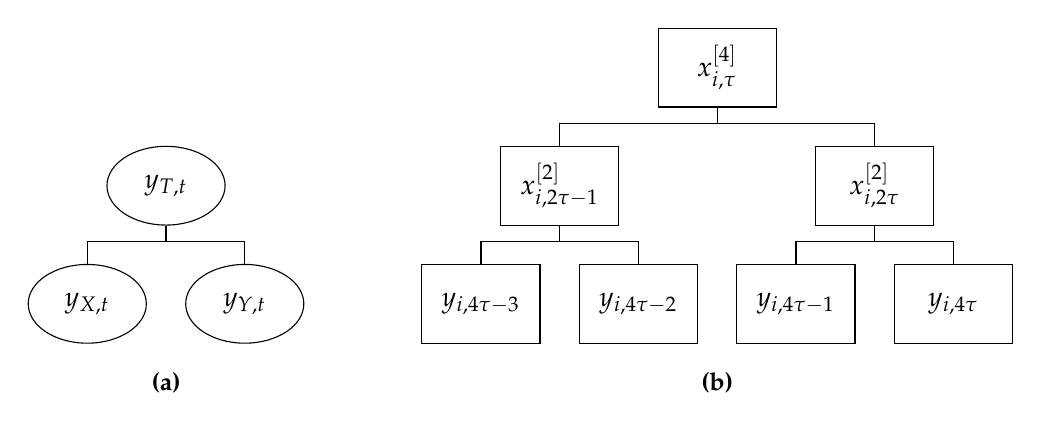
\begin{tikzpicture}[baseline=(current  bounding  box.center),
			rel/.append style={shape=ellipse,
				draw=black,
			minimum width=1.5cm,
			minimum height=1cm},
			rel2/.append style={shape=rectangle,
				draw=black,
			minimum width=1.5cm,
			minimum height=1cm},
			connection/.style ={inner sep =0, outer sep =0}]
			
			\node[rel] at (0, 0) (X){$y_{X,t}$};
			\node[rel] at (2, 0) (Y){$y_{Y,t}$};
			\node[rel] at (1, 1.5) (Tt){$y_{T,t}$};
			
			\relation{0.2}{X}{Tt};
			\relation{0.2}{Y}{Tt};
			
			
			\node[rel2] at (5, 0) (AA){$y_{i,4\tau-3}$};
			\node[rel2] at (7, 0) (AB){$y_{i,4\tau-2}$};
			\node[rel2] at (9, 0) (BA){$y_{i,4\tau-1}$};
			\node[rel2] at (11, 0) (BB){$y_{i,4\tau}$};
			
			\node[rel2] at (6, 1.5) (A){$x_{i,2\tau-1}^{[2]}$};
			\node[rel2] at (10, 1.5) (B){$x_{i,2\tau}^{[2]}$};
			\node[rel2] at (8, 3) (T){$x_{i,\tau}^{[4]}$};
			
			\node at (1, -1) (){\small \textbf{(a)}};
			\node at (8, -1) (){\small \textbf{(b)}};
			
			\relation{0.2}{AA}{A};
			\relation{0.2}{AB}{A};
			\relation{0.2}{BA}{B};
			\relation{0.2}{BB}{B};
			
			\relation{0.2}{A}{T};
			\relation{0.2}{B}{T};
		\end{tikzpicture}
		\caption{\textbf{(a)} A simple two-level cross-sectional hierarchy for 3 linearly constrained time series with $n=3$, $n_a = 1$ and $n_b = 2$. \textbf{(b)} A temporal hierarchy for a quarterly series ($m = 4$ and $\mathcal{K} = \{4,2,1\}$).}
\label{fig:hierS}
\end{figure}

Considering now the temporal framework, we denote with $\mathcal{K} = \{ k_p , k_{p-1}, \dots, k_2, k_1 \}$ the set of $p$ factors of $m$, in descending order, where $k_1= 1$ and $k_p= m$ \citep{athanasopoulos2017}. Given a factor $k$ of $m$ and assuming that $T = N m$ (where $N$ is the length of the most temporally aggregated version of the series), we can construct a temporally aggregated version of the time series of a single variable $\{\yvet_{i,t}\}_{t = 1, \dots, T}$, through the non-overlapping sums of its $k$ successive values, which has a seasonal period equal to $M_k= m/k$:
$$
x_{i,j}^{[k]} = \sum_{t=(j-1)k+1}^{jk} y_{i,t},\qquad j = 1,\dots, T/k, \qquad i = 1,\dots,n.
$$
Note that $x_{i,j}^{[1]}=y_{i,t}$. Define cycle $\tau$ as the observation index of the most aggregated level $k_p$. For a fixed temporal aggregation order $k \in \mathcal{K}$, we stack the observations in the column vector
$$
\xvet_{i,\tau}^{k} = \begin{bmatrix}x_{i,M_k(\tau-1)+1}^{[k]} & x_{i,M_k(\tau-1)+2}^{[k]} & \dots & x_{i,M_k\tau}^{[k]}\end{bmatrix}',
$$
and obtain the vector for all the aggregation orders
$$
\xvet_{i,\tau} = \begin{bmatrix}
	x_{i,\tau}^{[k_p]} &
	\xvet_{i,\tau}^{[k_{p-1}]\prime} &
	\dots &
	\xvet_{i,\tau}^{[1]\prime}
\end{bmatrix}'\quad \tau = 1,\dots,N.
$$
The structural representation of the temporal hierarchy \citep{athanasopoulos2017} is then
$$
\xvet_{i,\tau} = \Svet_{te}\xvet_{i,\tau}^{[1]},
$$
where $\Svet_{te} = \begin{bmatrix}\Avet_{te}' & \Ivet_{m}\end{bmatrix}'$ is the $[(m+k^\ast) \times m]$ temporal structural matrix, and
$$
\Avet_{te} = \begin{bmatrix}
	\multicolumn{3}{c}{\Unovet_{k_p}'}\\
	\Ivet_{\frac{m}{k_{p-1}}} & \otimes & \Unovet_{k_{p-1}}'\\
	&\vdots &\\
	\Ivet_{\frac{m}{k_{2}}} & \otimes & \Unovet_{k_2}'
\end{bmatrix}
$$
is the $(k^\ast \times m)$ temporal aggregation matrix with $k^\ast = \sum_{k \in \mathcal{K}\setminus\{k_1\}} m/k$. For each series $i = 1,\dots,n$, we have also the zero-constrained representation
\begin{equation}
\label{eq:te_con}
	\Cvet_{te}\xvet_{i,\tau} = \Zerovet_{[k^\ast \times (m+k^\ast)]}, \qquad \tau = 1,\dots,N, \qquad i = 1,\dots, n
\end{equation}
where $\Cvet_{te} = \begin{bmatrix}\Ivet_{k^\ast} & -\Avet_{te}\end{bmatrix}$ is the $\left[k^\ast \times (m+k^\ast)\right]$ zero constraints temporal matrix.
Figure \ref{fig:hierS}(b) shows the hierarchical representation of a quarterly time series, for which $m = 4$, $\mathcal{K} = \{4,2,1\}$, and
$$
\Avet_{te} = \begin{bmatrix}
	1 & 1 & 1 & 1\\
	1 & 1 & 0 & 0\\
	0 & 0 & 1 & 1\\
\end{bmatrix}, \quad \Cvet_{te} = \begin{bmatrix}
	1 & 0 & 0 & -1 & -1 & -1 & -1\\
	0 & 1 & 0 & -1 & -1 & 0 & 0\\
	0 & 0 & 1 & 0 & 0 & -1 & -1\\
\end{bmatrix} \quad \mathrm{and} \quad \Svet_{te} = \begin{bmatrix}
	\Avet_{te} \\
	\Ivet_4
\end{bmatrix}.
$$
When we temporally aggregate each series, the cross-sectional constraints for the most temporally disaggregated series (\ref{eq:cs_con}) hold for all the temporal aggregation orders
\begin{equation}
\label{eq:cs_con2}
	\Cvet_{cs}\xvet^{[k]}_t = \Zerovet_{(n_a \times 1)}, \quad \mathrm{for} \quad k \in \mathcal{K} \quad \mathrm{and} \quad t = 1, \;\dots, \;T,
\end{equation}
where $\xvet_t^{[k]} = \begin{bmatrix}
 \uvet_t^{[k]\prime} & \bvet_t^{[k]\prime}
 \end{bmatrix}'$ with $\uvet^{[k]}_t = \begin{bmatrix} x^{[k]}_{1,t} & \dots & x^{[k]}_{n_a,t}
\end{bmatrix}'$ is the $n_a$-vector of upper time series and $\bvet^{[k]}_t = \begin{bmatrix} x^{[k]}_{(n_a+1),t} & \dots & x^{[k]}_{n,t} \end{bmatrix}'$ is the $n_b$-vector of bottom time series in the temporal hierarchy.

\begin{figure}[!t]
  \centering
\begin{tikzpicture}
\tikzset{square matrix/.style={
    matrix of nodes,
    column sep=-\pgflinewidth, row sep=-\pgflinewidth,
    nodes={draw,
      minimum height=#1,
      anchor=center,
      text width=#1,
      align=center,
      inner sep=0pt,
      font=\scriptsize
    },
  },
  square matrix/.default=0.5cm
}

\matrix[square matrix](S)
{
|[fill=black]| & |[fill=black]| & |[draw=none]|$T$\\
|[fill=black]| & |[fill=white]| & |[draw=none]|$X$\\
|[fill=white]| & |[fill=black]| & |[draw=none]|$Y$\\
|[draw=none]|$X$ & |[draw=none]|$Y$ & |[draw=none]|$i$\\
};

\matrix[square matrix, right=of S](K)
{
|[fill=black]| & |[fill=black]| & |[fill=black]| & |[fill=black]| & |[draw=none]|$\quad x^{[4]}_{i,\tau}$\\
|[fill=black]| & |[fill=black]| & |[fill=white]| & |[fill=white]| & |[draw=none]|$\quad x^{[2]}_{i,2\tau-1}$\\
|[fill=white]| & |[fill=white]| & |[fill=black]| & |[fill=black]| & |[draw=none]|$\quad x^{[2]}_{i,2\tau}$\\
|[fill=black]| & |[fill=white]| & |[fill=white]| & |[fill=white]| & |[draw=none]|$\quad y^{\phantom{[1]}}_{i,4\tau-3}$\\
|[fill=white]| & |[fill=black]| & |[fill=white]| & |[fill=white]| & |[draw=none]|$\quad y^{\phantom{[1]}}_{i,4\tau-2}$\\
|[fill=white]| & |[fill=white]| & |[fill=black]| & |[fill=white]| & |[draw=none]|$\quad y^{\phantom{[1]}}_{i,4\tau-1}$\\
|[fill=white]| & |[fill=white]| & |[fill=white]| & |[fill=black]| & |[draw=none]|$\quad y^{\phantom{[1]}}_{i,4\tau}$\\
|[draw=none]| & |[draw=none]| & |[draw=none]| & |[draw=none]| & & \\
};

\node[right of=S,font=\bfseries,xshift = 0.35cm, font = \large] (kro) {$\bigotimes$};
%\node[fit=(K-8-2)(K-8-3), font=\scriptsize, yshift = -0.25cm]{$\yvet_{(\tau)}^{i,[1]}$};

\node[fit=(K-8-2)(K-8-3), font=\scriptsize, yshift = -0.25cm, text width=6cm]{$\xvet_{i,\tau}^{[1]}$}; %\\ \rotatebox{90}{$=\;$} \\$\left[y^{\phantom{[1]}}_{i,4\tau-3}\; y^{\phantom{[1]}}_{i,4\tau-2}\; y^{\phantom{[1]}}_{i,4\tau-1}\; y^{\phantom{[1]}}_{i,4\tau}\right]'$};

\node[right of=S,font=\bfseries,xshift = 4.85cm, font = \huge] (ugu) {$\mathbf{=}$};

\matrix[square matrix, right=of K,xshift = 0.5cm](St)
{
|[fill=black]| & |[fill=black]| & |[fill=black]| & |[fill=black]| & |[fill=black]| & |[fill=black]| & |[fill=black]| & |[fill=black]| & |[draw=none]|$\quad x^{[4]}_{T,\tau}$\\
|[fill=black]| & |[fill=black]| & |[fill=white]| & |[fill=white]| & |[fill=black]| & |[fill=black]| & |[fill=white]| & |[fill=white]| & |[draw=none]|$\quad x^{[2]}_{T,2\tau-1}$\\
|[fill=white]| & |[fill=white]| & |[fill=black]| & |[fill=black]| & |[fill=white]| & |[fill=white]| & |[fill=black]| & |[fill=black]| & |[draw=none]|$\quad x^{[2]}_{T,2\tau}$\\
|[fill=black]| & |[fill=white]| & |[fill=white]| & |[fill=white]| & |[fill=black]| & |[fill=white]| & |[fill=white]| & |[fill=white]| & |[draw=none]|$\quad y^{\phantom{[1]}}_{T,4\tau-3}$\\
|[fill=white]| & |[fill=black]| & |[fill=white]| & |[fill=white]| & |[fill=white]| & |[fill=black]| & |[fill=white]| & |[fill=white]| & |[draw=none]|$\quad y^{\phantom{[1]}}_{T,4\tau-2}$\\
|[fill=white]| & |[fill=white]| & |[fill=black]| & |[fill=white]| & |[fill=white]| & |[fill=white]| & |[fill=black]| & |[fill=white]| & |[draw=none]|$\quad y^{\phantom{[1]}}_{T,4\tau-1}$\\
|[fill=white]| & |[fill=white]| & |[fill=white]| & |[fill=black]| & |[fill=white]| & |[fill=white]| & |[fill=white]| & |[fill=black]| & |[draw=none]|$\quad y^{\phantom{[1]}}_{T,4\tau}$\\
|[fill=black]| & |[fill=black]| & |[fill=black]| & |[fill=black]| & |[fill=white]| & |[fill=white]| & |[fill=white]| & |[fill=white]| & |[draw=none]|$\quad x^{[4]}_{X,\tau}$\\
|[fill=black]| & |[fill=black]| & |[fill=white]| & |[fill=white]| & |[fill=white]| & |[fill=white]| & |[fill=white]| & |[fill=white]| & |[draw=none]|$\quad x^{[2]}_{X,2\tau-1}$\\
|[fill=white]| & |[fill=white]| & |[fill=black]| & |[fill=black]| & |[fill=white]| & |[fill=white]| & |[fill=white]| & |[fill=white]| & |[draw=none]|$\quad x^{[2]}_{X,2\tau}$\\
|[fill=black]| & |[fill=white]| & |[fill=white]| & |[fill=white]| & |[fill=white]| & |[fill=white]| & |[fill=white]| & |[fill=white]| & |[draw=none]|$\quad y^{\phantom{[1]}}_{X,4\tau-3}$\\
|[fill=white]| & |[fill=black]| & |[fill=white]| & |[fill=white]| & |[fill=white]| & |[fill=white]| & |[fill=white]| & |[fill=white]| & |[draw=none]|$\quad y^{\phantom{[1]}}_{X,4\tau-2}$\\
|[fill=white]| & |[fill=white]| & |[fill=black]| & |[fill=white]| & |[fill=white]| & |[fill=white]| & |[fill=white]| & |[fill=white]| & |[draw=none]|$\quad y^{\phantom{[1]}}_{X,4\tau-1}$\\
|[fill=white]| & |[fill=white]| & |[fill=white]| & |[fill=black]| & |[fill=white]| & |[fill=white]| & |[fill=white]| & |[fill=white]| & |[draw=none]|$\quad y^{\phantom{[1]}}_{X,4\tau}$\\
|[fill=white]| & |[fill=white]| & |[fill=white]| & |[fill=white]| & |[fill=black]| & |[fill=black]| & |[fill=black]| & |[fill=black]| & |[draw=none]|$\quad x^{[4]}_{Y,\tau}$\\
|[fill=white]| & |[fill=white]| & |[fill=white]| & |[fill=white]| & |[fill=black]| & |[fill=black]| & |[fill=white]| & |[fill=white]| & |[draw=none]|$\quad x^{[2]}_{Y,2\tau-1}$\\
|[fill=white]| & |[fill=white]| & |[fill=white]| & |[fill=white]| & |[fill=white]| & |[fill=white]| & |[fill=black]| & |[fill=black]| & |[draw=none]|$\quad x^{[2]}_{Y,2\tau}$\\
|[fill=white]| & |[fill=white]| & |[fill=white]| & |[fill=white]| & |[fill=black]| & |[fill=white]| & |[fill=white]| & |[fill=white]| & |[draw=none]|$\quad y^{\phantom{[1]}}_{Y,4\tau-3}$\\
|[fill=white]| & |[fill=white]| & |[fill=white]| & |[fill=white]| & |[fill=white]| & |[fill=black]| & |[fill=white]| & |[fill=white]| & |[draw=none]|$\quad y^{\phantom{[1]}}_{Y,4\tau-2}$\\
|[fill=white]| & |[fill=white]| & |[fill=white]| & |[fill=white]| & |[fill=white]| & |[fill=white]| & |[fill=black]| & |[fill=white]| & |[draw=none]|$\quad y^{\phantom{[1]}}_{Y,4\tau-1}$\\
|[fill=white]| & |[fill=white]| & |[fill=white]| & |[fill=white]| & |[fill=white]| & |[fill=white]| & |[fill=white]| & |[fill=black]| & |[draw=none]|$\quad y^{\phantom{[1]}}_{Y,4\tau}$\\
|[draw=none]| & |[draw=none]| & |[draw=none]| & |[draw=none]| & |[draw=none]| & |[draw=none]| & |[draw=none]| & |[draw=none]| & \\
};

\node[fit=(St-22-1)(St-22-8), font=\scriptsize, yshift = -0.25cm, text width=6cm]{$\bvet_{\tau}^{[1]}$};

\node[fit=(St-1-9)(St-21-9), draw = black, xshift = 0.6cm, minimum width = 1.3cm, label={[font=\scriptsize,text=black]above:{$\xvet_{\tau}$}}]{};

\node[fit=(K-1-5)(K-7-5), draw = black, xshift = 0.5cm, minimum width = 1.2cm, label={[font=\scriptsize,text=black]above:{$\xvet_{i,\tau}$}}]{};

\node[fit=(K-1-1.north west)(K-2-4.south east), label={[font=\normalsize,text=black]above:{$\Svet_{te}$}}]{};

\node[fit=(St-1-1.north west)(St-2-8.south east), label={[font=\normalsize,text=black]above:{$\Svet_{ct}$}}]{};

\node[fit=(S-1-1.north west)(S-2-2.south east), label={[font=\normalsize,text=black]above:{$\Svet_{cs}$}}]{};

\draw[ultra thick,decorate,decoration={calligraphic brace,amplitude=7.5pt}] ($(St-1-9.north)+(1.35,-0.1)$) -- node[right, rotate = -90, anchor = center, align = center, text width = 2.5cm, yshift = 0.75cm, font = \footnotesize] {Temporal components of $T$} ($(St-7-9.south)+(1.35,0.05)$);

\draw[ultra thick,decorate,decoration={calligraphic brace,amplitude=7.5pt}] ($(St-8-9.north)+(1.35,-0.1)$) -- node[right, rotate = -90, anchor = center, align = center, text width = 2.5cm, yshift = 0.75cm, font = \footnotesize] {Temporal components of $X$} ($(St-14-9.south)+(1.35,0.05)$);

\draw[ultra thick,decorate,decoration={calligraphic brace,amplitude=7.5pt}] ($(St-15-9.north)+(1.35,-0.1)$) -- node[right, rotate = -90, anchor = center, align = center, text width = 2.5cm, yshift = 0.75cm, font = \footnotesize] {Temporal components of $Y$} ($(St-21-9.south)+(1.35,0.05)$);
\end{tikzpicture}
\vspace{-0.25cm}
  \caption{Visual representation of the cross-temporal summation matrix $\Svet_{ct} = \Svet_{cs} \otimes \Svet_{te}$ defined in (\ref{eq:Sct}) for a system of 3 linearly constrained quarterly time series (see \autoref{fig:hierS}). Colours legend: 0s in white, 1s in black.}
  \label{fig:Stilde}
\end{figure}


To include both cross-sectional and temporal constraints at the same time in a unified framework, we stack the series into a $\left[n \times (m+k^\ast)\right]$ matrix $\Xvet_\tau$, whose rows and columns represent, respectively, the cross-sectional and the temporal dimension:
\begin{equation}
\label{eq:Xtau}
\Xvet_\tau = \begin{bmatrix}
	\xvet_{1,\tau}'\\
	\vdots \\
	\xvet_{n,\tau}'
\end{bmatrix} = \begin{bmatrix}
\Xvet_{\tau}^{[k_p]} & \dots & \Xvet_{\tau}^{[k_1]} \\ \end{bmatrix}
\quad \text{with} \quad \Xvet_{\tau}^{[k]} = \begin{bmatrix}
	\Uvet_{\tau}^{[k]} \\
	\Bvet_{\tau}^{[k]},
\end{bmatrix}
%= \begin{bmatrix}
%\Uvet_{\tau}^{[k_p]} & \dots & \Uvet_{\tau}^{[k_1]} \\[0.25cm]
%\Bvet_{\tau}^{[k_p]} & \dots & \Bvet_{\tau}^{[k_1]} \\ \end{bmatrix}
\end{equation}
where for any fixed $k$,
$\Uvet_{\tau}^{[k]}$ is the ($n_a\times T/k$) matrix grouping the upper time series, $\Bvet_{\tau}^{[k]}$ is the ($n_b\times T/k$) matrix grouping the bottom time series. In addition, it is
$$
\Cvet_{cs}\Xvet_\tau = \Zerovet_{\left[n_a \times (m+k^\ast)\right]} \qquad \text{and} \qquad \Cvet_{te}\Xvet_\tau' = \Zerovet_{(k^\ast \times n)} .
$$
\cite{difonzo2023} show that the cross-temporal constraints working on the complete set of observations at cycle $\tau$ can be expressed in the zero-constrained representation through the $\left[(n_am+nk^\ast)\times n(m+k^\ast)\right]$ zero constraints cross-temporal kernel matrix $\Cvet_{ct}$ such that
\begin{equation}
\label{eq:Cct}
	\Cvet_{ct} = \begin{bmatrix}
	\Cvet_\ast\\
	\Ivet_n \otimes \Cvet_{te}
\end{bmatrix} \quad \Longrightarrow \quad
\Cvet_{ct} \xvet_{\tau} = \Zerovet_{[(n_am+nk^\ast)\times1]} \quad \mathrm{for} \quad \tau = 1,\dots,N,
\end{equation}
where
$\xvet_{\tau} = \mathrm{vec}\left(\Xvet_{\tau}'\right) = \begin{bmatrix}
	\xvet_{1, \tau}' &
	\dots &
	\xvet_{n, \tau}'
\end{bmatrix}'$, %($\mathrm{vec}(\cdot)$ is the “vectorization" operator),
$\Cvet_\ast = \begin{bmatrix}\Zerovet_{(n_a m\times nk^\ast)} & \Ivet_m \otimes \Cvet_{cs}\end{bmatrix}\Pvet'$ and $\Pvet$ is the commutation matrix (\citealp{magnus2019}, p. 54) $\Pvet \mathrm{vec}\left(\Yvet_{\tau}\right) = \mathrm{vec}\left(\Yvet_{\tau}'\right)$. A structural representation can be considered as well:
$$
\xvet_\tau = \Svet_{ct}\bvet^{[1]}_\tau = s\left(\bvet_{\tau}^{[1]}\right),
$$
where
\begin{equation}
	\label{eq:Sct}
	\Svet_{ct} = \Svet_{cs} \otimes \Svet_{te}
\end{equation}
is the $\left[n(k^\ast+m)\times n_b m\right]$ cross-temporal summation matrix, $s: \mathbb{R}^{n_b m} \rightarrow \mathbb{R}^{n(m+k^\ast)}$ is the operator describing the pre-multiplication by $\Svet_{ct}$, and $\bvet^{[1]}_\tau = \mathrm{vec}\left(\Bvet^{[1]\prime}_{\tau}\right)$. We observe that, in agreement with \cite{panagiotelis2021}, $\xvet_{\tau}$ lies in an $(n_b m)$-dimensional subspace $\mathfrak{s}_{ct}$ of $\mathbb{R}^{n(k^\ast+m)}$, which we refer to as “cross-temporal coherent subspace”, spanned by the columns of $\Svet_{ct}$.
In Figure \ref{fig:Stilde}, we have represented $\Svet_{ct}$ for 3 linearly constrained quarterly time series, like Figure \ref{fig:hierS}.

%\section{Point forecast reconciliation}\label{sec:point}

\subsection{Optimal point forecast reconciliation}\label{ssec:oct}
%Given a set of incoherent, however obtained, base forecasts for a system of hierarchical time series, forecast reconciliation is in practice a post-forecasting process aimed to improve the quality of the base forecasts.

Let $\widehat{\xvet}_{h} = \mathrm{vec}\left(\widehat{\Xvet}_{h}'\right)$, $h = 1, \dots, H$, be the base forecasts (however obtained) where $H$ is the forecast horizon for the most temporally aggregated time series. Denote
$$
	\widehat{\Xvet}_{h} = \begin{bmatrix}
	\widehat{\xvet}_{1,h}\\
	\vdots\\
	\widehat{\xvet}_{n,h}
\end{bmatrix} =\begin{bmatrix}
\widehat{\Uvet}_{h}^{[m]} & \dots & \widehat{\Uvet}_{h}^{[k]} & \dots & \widehat{\Uvet}_{h}^{[1]} \\[0.25cm]
\widehat{\Bvet}_{h}^{[m]} & \dots & \widehat{\Bvet}_{h}^{[k]} & \dots & \widehat{\Bvet}_{h}^{[1]} \\ \end{bmatrix},
$$
where $\widehat{\Uvet}_{h}^{[k]}$ is the ($n_a\times M_k$) matrix grouping the upper time series and $\widehat{\Bvet}_{h}^{[k]}$ is the ($n_b\times M_k$) matrix grouping the bottom time series for a given temporal aggregation order $k$. The matrix $\widehat{\Xvet}_{h}$, organized as ${\Xvet}_{\tau}$ in expression (\ref{eq:Xtau}), contains incoherent forecasts, that is:
$$
\Cvet_{ct} \widehat{\xvet}_{h} \neq \Zerovet_{[(n_am+nk^\ast)\times1]} \quad h = 1, \dots, H
$$
with $\widehat{\xvet}_{h} = \mathrm{vec}\left(\widehat{\Xvet}_{h}'\right)$. In this framework, the definition for the forecast reconciliation in the cross-sectional framework given by \cite{panagiotelis2021} can be generalized as follows.
\begin{definition}
	The forecast reconciliation aims to adjust the base forecast $\widehat{\xvet}_{h}$ finding a mapping $\psi: \mathbb{R}^{n(m+k^\ast)} \rightarrow \mathfrak{s}$ such that $\widetilde{\xvet}_{h} = \psi\left(\widehat{\xvet}_{h}\right)$, where $\widetilde{\xvet}_{h} \in \mathfrak{s}$ is the vector of the reconciled forecasts.
\end{definition}

For a given forecast horizon $h = 1,\dots, H$, the mapping $\psi$ may be defined as the solution to the multivariate regression model (\citealp{difonzo2023})
$$
\widehat{\Xvet}_{h} = \Xvet_{h} + \Evet_{h},
$$
where the involved matrices have each dimension $[n \times (k^\ast + m)]$ and contain, respectively, the base $\Big(\widehat{\Xvet}_{h}\Big)$ and the target forecasts $\Big(\Xvet_{h}\Big)$, and the coherency errors $\Big(\Evet_{h}\Big)$. We consider now the vectorized version of this multivariate model, such that
$$
\widehat{\xvet}_{h} = \xvet_{h} + \etavet_{h}
$$
where $\widehat{\xvet}_{h} = \mathrm{vec}\Big(\widehat{\Xvet}'_{h}\Big)$, $\xvet_{h} = \mathrm{vec}\Big(\Xvet'_{h}\Big)$ and $\etavet_{h} = \mathrm{vec}\Big(\Evet'_{h}\Big)$  is the cross-temporal reconciliation error with zero mean and p.d. covariance matrix $\Omegavet_{ct}$.
Assuming $\Omegavet_{ct}$ known, the reconciled forecasts are the solution to the linearly constrained minimization of the generalized least squares (GLS) objective function
$$
\left(\xvet_h - \widehat{\xvet}_h\right)' \Omegavet_{ct}^{-1}\left(\xvet_h - \widehat{\xvet}_h\right)  \qquad \text{s.t.} \quad \Cvet_{ct}\xvet_h = \Zerovet_{[(n_am+nk^\ast)\times1]}.
$$
According to the projection approach \citep{byron1978,byron1979, vanerven2015, wickramasuriya2019, panagiotelis2021, difonzo2023}, the cross-temporally reconciled forecasts are then given by
\begin{equation}
	\label{eq:Mvet}
	\widetilde{\xvet}_{h} = \psi\left(\widehat{\xvet}\right) = \Mvet \widehat{\xvet},
\end{equation}
where $\Mvet = \Ivet_{n(m+ k^\ast)} - \Omegavet_{ct}\Cvet'_{ct}\left(\Cvet_{ct}\Omegavet_{ct}\Cvet'_{ct}\right)^{-1}\Cvet_{ct}$, and $\widetilde{\xvet}_{h} = \mathrm{vec}\Big(\widetilde{\Xvet}'_{h}\Big)$. It is worth noting that $\Cvet_{ct}$ defined in equation (\ref{eq:Cct}) is a full rank matrix.

Alternatively, the cross-temporal reconciled forecasts $\widetilde{\Xvet}_{h}$ may be found according to the structural approach proposed by \cite{hyndman2011} for the cross-sectional framework, then extend in terms of minimum variance linear unbiased reconciled forecasts \citep{wickramasuriya2019}:
$$
\min_{\Gvet} \; \text{tr}\left(\Svet_{ct}\Gvet\Omegavet_{ct}\Gvet'\Svet_{ct}' \right) \quad \text{s.t.} \; \Svet_{ct}\Gvet\Svet_{ct} = \Svet_{ct},
$$
with solution equivalent to the cross-temporally reconciled forecasts in (\ref{eq:Mvet}), given by
\begin{equation}\label{eq:SGy}
	\widetilde{\xvet}_{h} = \psi\left(\widehat{\xvet}\right) = \left(s \circ g \right)\left(\widehat{\xvet}\right)=\Svet_{ct}\Gvet \widehat{\xvet}_{h},
\end{equation}
where $\Gvet = \left(\Svet_{ct}' \Omegavet_{ct}^{-1}\Svet_{ct}\right)^{-1} \Svet_{ct}'\Omegavet_{ct}^{-1}$ and $\Mvet = \Svet_{ct} \Gvet$ \citep{wickramasuriya2019, difonzo2023}. In this case, $\psi$ is the composition of two transformations, say $s \circ g$, where $g: \mathbb{R}^{n(m+k^\ast)} \rightarrow \mathbb{R}^{n_b m}$ is a continuous function.

\cite{difonzo2023} consider the following approximations for the cross-temporal covariance matrix:
\begin{itemize}[nosep, leftmargin=!, labelwidth=\widthof{ oct$(bdsam)$ -}, align=right]
	\item[oct$(ols)$ -] identity: $\Omegavet_{ct} = \Ivet_{n(k^*+m)}$
	\item[oct$(struc)$ -] structural: $\Omegavet_{ct} = \mathrm{diag}(\Svet_{ct} \mathbf{1}_{mn_b})$
	\item[oct$(wlsv)$ -] series variance scaling: $\Omegavet_{ct} = \widehat{\Omegavet}_{ct,wlsv}$, that is a straightforward extension of the series variance scaling matrix presented by \cite{athanasopoulos2017} in the temporal framework
	\item[oct$(bdshr)$ -] block-diagonal shrunk cross-covariance scaling: $\Omegavet_{ct} = \Pvet\widehat{\Wvet}^{BD}_{ct,shr}\Pvet'$, with
	$$
	\widehat{\Wvet}^{BD}_{ct,shr} = \begin{bmatrix}
		\widehat{\Wvet}^{[m]}_{shr} & \Zerovet &\dots & \Zerovet\\
		\Zerovet & \hspace{10pt}\Ivet_{\frac{m}{k_{p-1}}} \otimes \widehat{\Wvet}^{[k_{p-1}]}_{shr} &\dots & \Zerovet \\
		 \vdots & \vdots & \ddots & \vdots\\
		 \Zerovet & \Zerovet & \dots & \hspace{15pt}\Ivet_{m} \otimes \widehat{\Wvet}^{[1]}_{shr} \\
	\end{bmatrix}
	$$
	a block diagonal matrix where $\widehat{\Wvet}^{[k]}_{shr}$ is the shrunk cross-sectional estimates of matrix proposed by \cite{wickramasuriya2019} fixed the temporal aggregation level $k$.
	%\item[oct$(bdsam)$ -] block-diagonal cross-covariance scaling: $\Omegavet_{ct} = \Pvet\widehat{\Wvet}^{BD}_{ct,sam}\Pvet'$
	\item[oct$(shr)$ -] MinT-shr:   $\Omegavet_{ct} = \hat{\lambda}\widehat{\Omegavet}_{ct,D} + (1-\hat{\lambda})\widehat{\Omegavet}_{ct}$
	\item[oct$(sam)$ -] MinT-sam:  $\Omegavet_{ct} = \widehat{\Omegavet}_{ct}$
\end{itemize}
where the symbol $\odot$ denotes the Hadamard product, $\hat{\lambda}$ is an estimated shrinkage coefficient (\citealp{ledoit2004a}), $\widehat{\Omegavet}_{ct,D} = \Ivet_{n(k^\ast + m)} \odot \widehat{\Omegavet}_{ct}$, and $\widehat{\Omegavet}_{ct}$ is the covariance matrix of the cross-temporal one-step ahead in-sample forecast errors.

We can consider the cross-temporal framework as a generalization of the cross-sectional and temporal ones, that takes simultaneously into account both types of constraints. In addition, the cross-sectional reconciliation approach proposed by \cite{hyndman2011} can be obtained by assuming $m = 1$, while the temporal one \citep{athanasopoulos2017} is obtained when $n = 1$ (with $n_a = 0$ and $n_b = 1$). Table \ref{tab:cov_app} presents some approximations for the cross-sectional and the temporal covariance matrices. \cite{nystrup2020} and \cite{difonzo2023} provide further temporal reconciliation approaches that exploit possible information in the residuals' autocorrelation.

\begin{table}[bt]
  \caption{Approximations for the cross-sectional (\citealp{hyndman2011}, \citealp{hyndman2016}, \citealp{wickramasuriya2019}, \citealp{difonzo2023}) and temporal (\citealp{athanasopoulos2017}, \citealp{difonzo2023}) covariance matrix, respectively $\Wvet$ and $\Omegavet$.}
  \label{tab:cov_app}
\centering
\footnotesize
  \begin{tabular}{>{\raggedleft\arraybackslash}m{0.15\linewidth}|>{\centering\arraybackslash}m{0.35\linewidth}|>{\centering\arraybackslash}m{0.35\linewidth}}
  \toprule
    & \textbf{Cross-sectional framework} & \textbf{Temporal framework} \\
    \midrule
    identity & cs$(ols)$: $\Wvet = \Ivet_n$ & te$(ols)$: $\Omegavet = \Ivet_{k^\ast + m}$\\[0.1cm]
    structural & cs$(struc)$: $\Wvet = \mathrm{diag}(\Svet_{cs} \mathbf{1}_{nb})$ & te$(struc)$: $\Omegavet = \mathrm{diag}(\Svet_{te} \mathbf{1}_{m})$\\[0.1cm]
    series variance & cs$(wls)$: $\Wvet = \widehat{\Wvet}_D = \Ivet_n \odot \widehat{\Wvet}$ & te$(wlsv)$: $\Omegavet = \widehat{\Omegavet}_{wlsv}$\\[0.1cm]
    MinT-shr & cs$(shr)$: $\Wvet = \hat{\lambda}\widehat{\Wvet}_D + (1-\hat{\lambda})\widehat{\Wvet}$ & te$(shr)$: $\Omegavet = \hat{\lambda}\widehat{\Omegavet}_D + (1-\hat{\lambda})\widehat{\Omegavet}$\\[0.1cm]
    MinT-sam & cs$(sam)$: $\Wvet = \widehat{\Wvet}$ & te$(sam)$: $\Omegavet = \widehat{\Omegavet}$ \\
    \bottomrule \addlinespace[0.1cm]
    \multicolumn{3}{p{0.9\linewidth}}{\footnotesize \textbf{Note:} $\widehat{\Wvet}$ ($\widehat{\Omegavet}$) is the covariance matrix of the cross-sectional (temporal) one-step ahead in-sample forecast errors, $\widehat{\Omegavet}_{wlsv}$ is a diagonal matrix presented by \cite{athanasopoulos2017}, and $\widehat{\Omegavet}_D = \Ivet_{k^\ast + m} \odot \widehat{\Omegavet}$.}
  \end{tabular}
\end{table}

\subsection{Cross-temporal bottom-up forecast reconciliation}\label{ssec:ctbu}

The original classic bottom-up approach \citep{dunn1976, dangerfield1992} simply consists in summing-up the base forecasts of the most disaggregated level in the hierarchy to obtain upper-level series’ forecasts. To reduce the computational cost involved in optimal cross-temporal reconciliation, we may be interested in applying a reconciliation along only one dimension (cross-sectional or temporal) and reconstructing the cross-temporal structure using a partly bottom-up approach \citep{difonzo2022b, difonzo2023a, sanguri2022}.

Figure \ref{fig:bigBU} gives a visual representation of partly bottom-up as a two-step cross-temporal reconciliation approach. On the left (Figure \ref{fig:tebu}), we first compute the cross-sectionally reconciled forecasts at the highest frequency ($k = 1$), and then apply the temporal bottom-up to each series' forecasts.

On the right (Figure \ref{fig:csbu}), we first compute the temporally reconciled forecasts for the most disaggregated cross-sectional level, and then apply the cross-sectional bottom-up approach. We denote this two-step reconciliation as, respectively, ct$(rec_{te},bu_{cs})$, and ct$(rec_{cs},bu_{te})$, where ‘$rec_{te}$’ and ‘$rec_{cs}$’ denote a generic forecast reconciliation approach in the temporal and in cross-sectional framework.

\begin{figure}[t]
     \centering

    \begin{subfigure}[b]{0.49\textwidth}
	\centering
	\caption{$\widetilde{\Xvet}$ with ct$(rec_{cs}, bu_{te})$}
	\resizebox{\linewidth}{!}{
	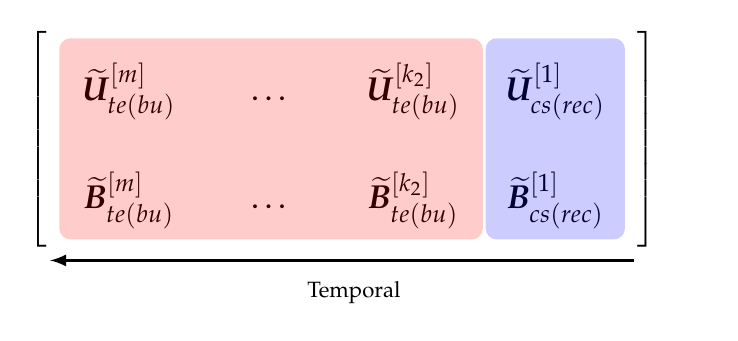
\begin{tikzpicture}[>=latex, line width=1pt,
		Matrix/.style={
            matrix of nodes,
            font=\large,
            align=center,
            text width = 1.5cm,
            text height = 0.65cm,
            column sep=2pt,
            row sep=7pt,
            nodes in empty cells,
            left delimiter={[},
            right delimiter={]},
            ampersand replacement=\&
		}]
		\matrix[Matrix] (Mt){ % Matrix contents
			$\widetilde{\Uvet}_{te(bu)}^{[m]}$ \& \dots \& $\widetilde{\Uvet}_{te(bu)}^{[k_2]}$ \& $\widetilde{\Uvet}_{cs(rec)}^{[1]}$ \\
			$\widetilde{\Bvet}^{[m]}_{te(bu)}$ \& \dots \& $\widetilde{\Bvet}^{[k_2]}_{te(bu)}$ \& $\widetilde{\Bvet}^{[1]}_{cs(rec)}$ \\
		};
		\draw[<-, opacity = 0] (Mt.north east)++(0.4,0) coordinate (temp) -- (temp |- Mt.south) node [midway,label={[label distance=0.1cm,rotate=-90, xshift = 1.5mm, font=\footnotesize]Cross-sectional}]{};
		\draw[<-] (Mt.south west)++(0,-0.15) coordinate (temp) -- (temp -| Mt.east) node [midway,label={[label distance=0cm,xshift = 1.5mm, font=\footnotesize]below:Temporal}]{};
		%\begin{scope}[on background layer]
		\node[opacity=0.2,
		rounded corners,
		inner sep=0pt, fill = blue, fit=(Mt-1-4)(Mt-2-4)](Bt){};
		\node[opacity=0.2,
		rounded corners,
		inner sep=0pt, fill = red, fit=(Mt-1-1)(Mt-2-3)](At){};
		%\end{scope}
	\end{tikzpicture}}
	%\vspace{-0.8cm}
	%\vskip0.25cm
	\label{fig:tebu}
	\end{subfigure}
     \hfill
      \begin{subfigure}[b]{0.49\textwidth}
	\centering
	\caption{$\widetilde{\Xvet}$ with ct$(rec_{te}, bu_{cs})$}
	\resizebox{\linewidth}{!}{
	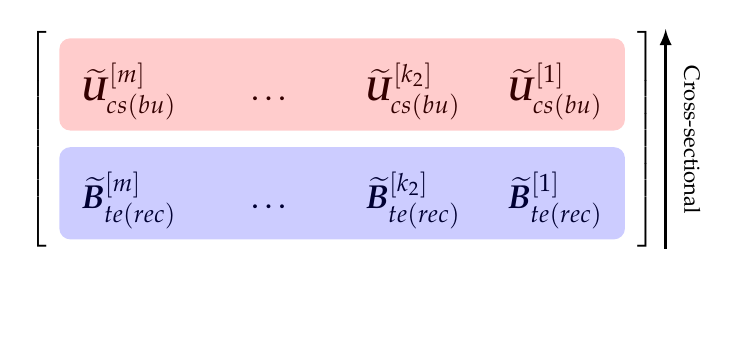
\begin{tikzpicture}[>=latex, line width=1pt,
		Matrix/.style={
            matrix of nodes,
            font=\large,
            align=center,
            text width = 1.5cm,
            text height = 0.65cm,
            column sep=2pt,
            row sep=7pt,
            nodes in empty cells,
            left delimiter={[},
            right delimiter={]},
            ampersand replacement=\&
		}]
		\matrix[Matrix] (Mcs){ % Matrix contents
			$\widetilde{\Uvet}_{cs(bu)}^{[m]}$ \& \dots \& $\widetilde{\Uvet}_{cs(bu)}^{[k_2]}$ \& $\widetilde{\Uvet}_{cs(bu)}^{[1]}$ \\
			$\widetilde{\Bvet}^{[m]}_{te(rec)}$ \& \dots \& $\widetilde{\Bvet}^{[k_2]}_{te(rec)}$ \& $\widetilde{\Bvet}^{[1]}_{te(rec)}$ \\
		};
		\draw[<-] (Mcs.north east)++(0.4,0) coordinate (temp) -- (temp |- Mcs.south) node [midway,label={[label distance=0.1cm,rotate=-90, xshift = 1.5mm, font=\footnotesize]Cross-sectional}]{};
		\draw[<-, opacity = 0] (Mcs.south west)++(0,-0.15) coordinate (temp) -- (temp -| Mcs.east) node [midway,label={[label distance=0cm,xshift = 1.5mm, font=\footnotesize]below:Temporal}]{};
		%\begin{scope}[on background layer]
		\node[opacity=0.2,
		rounded corners,
		inner sep=0pt, fill = blue, fit=(Mcs-2-1)(Mcs-2-4)](Bcs){};
		\node[opacity=0.2,
		rounded corners,
		inner sep=0pt, fill = red, fit=(Mcs-1-1)(Mcs-1-4)](Acs){};
		%\end{scope}
	\end{tikzpicture}}
	%\vspace{-0.8cm}
	%\vskip0.25cm
	\label{fig:csbu}
	\end{subfigure}
	\vspace{-1cm}
        \caption{A visual representation of partly bottom up starting from (\ref{fig:tebu}) cross-sectionally reconciled forecasts for the temporal order 1 $\left(\widetilde{\Uvet}^{[1]}\mbox{ and }\widetilde{\Bvet}^{[1]}\right)$ follow by a temporal bottom up, and (\ref{fig:csbu}) temporally reconciled forecasts of the cross-sectional bottom time series $\left(\widetilde{\Bvet}^{[k]}, \, k\in \mathcal{K}\right)$ follow by a cross-sectional bottom up. The \colorbox{mybluehl}{blue} background indicates the reconciliation along one dimension, while the \colorbox{pink}{pink} background indicates the forecasts obtained using bottom-up along the other dimension.}
        \label{fig:bigBU}
\end{figure}

\section{Probabilistic forecast reconciliation}\label{sec:prob}

To introduce the idea of coherence and probabilistic forecast reconciliation, we adapt to the cross-temporal framework the notations and the formal definitions introduced in \cite{wickramasuriya2021b} and \cite{panagiotelis2023} for the cross-sectional probabilistic case. These definitions can also be generalized by following the approach developed by \cite{corani2022} for count data. However, in this paper we only focus on the continuous case.

We want to extend the definition of \textit{cross-temporal coherent probabilistic forecasts} and \textit{cross-temporal probabilistic forecast reconciliation}.
Let $\left(\mathbb{R}^{n_b m}, \mathcal{F}_{\mathbb{R}^{n_b m}}, \mu\right)$ be a probability space for the high frequency bottom time series ($\bvet_{\tau}^{[1]}$), where $\mathcal{F}_{\mathbb{R}^{n_b m}}$ is the Borel $\sigma$-algebra on $\mathbb{R}^{n_b m}$. Then a $\sigma$-algebra $\mathcal{F}_{\mathfrak{s}}$ can be constructed from the collection of sets $s(\mathcal{B})$ for all $\mathcal{B} \in \mathcal{F}_{\mathbb{R}^{n_b m}}$.
\begin{definition}[Cross-temporal coherent probabilistic forecasts]
	Given the probability space $\left(\mathbb{R}^{n_b m}, \mathcal{F}_{\mathbb{R}^{n_b m}}, \mu\right)$, we call coherent probability space the triple $\left(\mathfrak{s}, \mathcal{F}_{\mathfrak{s}}, \breve{\mu}\right)$ satisfying the following property:
$$
\breve{\mu}(s(\mathcal{B}))=\mu(\mathcal{B}), \quad \forall \mathcal{B} \in \mathcal{F}_{\mathbb{R}^{n_b m}} .
$$
\end{definition}
Let $\left(\mathbb{R}^{n(m+k^\ast)}, \mathcal{F}_{\mathbb{R}^{n(m+k^\ast)}}, \hat{\mu}\right)$ be a probability space referring to the incoherent probabilistic forecast ($\widehat{\xvet}_{h}$) for all the $n$ series at any temporal aggregation $k \in \mathcal{K}$ in the system.
\begin{definition}[Cross-temporal probabilistic forecast reconciliation]\label{def:pfr}
The reconciled probability measure of $\hat{\mu}$ with respect to $\psi$ is a probability measure $\tilde{\mu}$ on $\mathfrak{s}$ with $\sigma$-algebra $\mathcal{F}_{\mathfrak{s}}$ satisfying
\begin{equation}\label{eq:pfr}
	\tilde{\mu}(\mathcal{A})=\hat{\mu}\left(\psi^{-1}(\mathcal{A})\right), \quad \forall \mathcal{A} \in \mathcal{F}_{\mathfrak{s}},
\end{equation}
where $\psi^{-1}(\mathcal{A})=\left\{x \in \mathbb{R}^{n(m+k^\ast)}: \psi(x) \in \mathcal{A}\right\}$ denotes the pre-image of $\mathcal{A}$.
\end{definition}
The map $\psi$ may be obtained as the composition of $s \circ g$, as for the cross-temporal point reconciliation (\ref{eq:SGy}).

In the same way, the definitions and theorems presented in \citet{corani2021} for a more general framework valid also for count data ($\mathbb{N}$) can be applied to the cross-temporal case as well.

%\listoftodos[Notes]

\subsection{Non-parametric framework: bootstrap reconciliation}\label{ssec:boot}

Analytical expressions for the base and reconciled forecast distributions are sometimes challenging to express, or use unrealistic parametric assumptions.

\begin{theorem}[Cross-temporal reconciled samples] \label{thm:rs}
	Suppose that $\left(\widehat{\xvet}_1, \ldots, \widehat{\xvet}_L\right)$ is a sample drawn from a (cross-temporal) incoherent probability measure $\widehat{\nu}$. Then $\left(\widetilde{\xvet}_1, \ldots, \widetilde{\xvet}_L\right)$, where $\widetilde{\xvet}_\ell:=\psi\left(\widehat{\xvet}_\ell\right)$, $\ell= 1, \ldots, L\;$, is a sample drawn from the (cross-temporal) reconciled probability measure $\widetilde{\nu}$ as defined in (\ref{eq:pfr}).
\end{theorem}
\begin{proof}
	See Theorem 4.5 from \cite{panagiotelis2023} using Definition \ref{def:pfr}.
\end{proof}
Theorem \ref{thm:rs} is the cross-temporal extension of the Theorem 4.5 in \cite{panagiotelis2023}. It means that a sample from the reconciled distribution can be obtained by reconciling each member of a sample from the incoherent distribution.

\begin{figure}[!hbp]
	\centering
	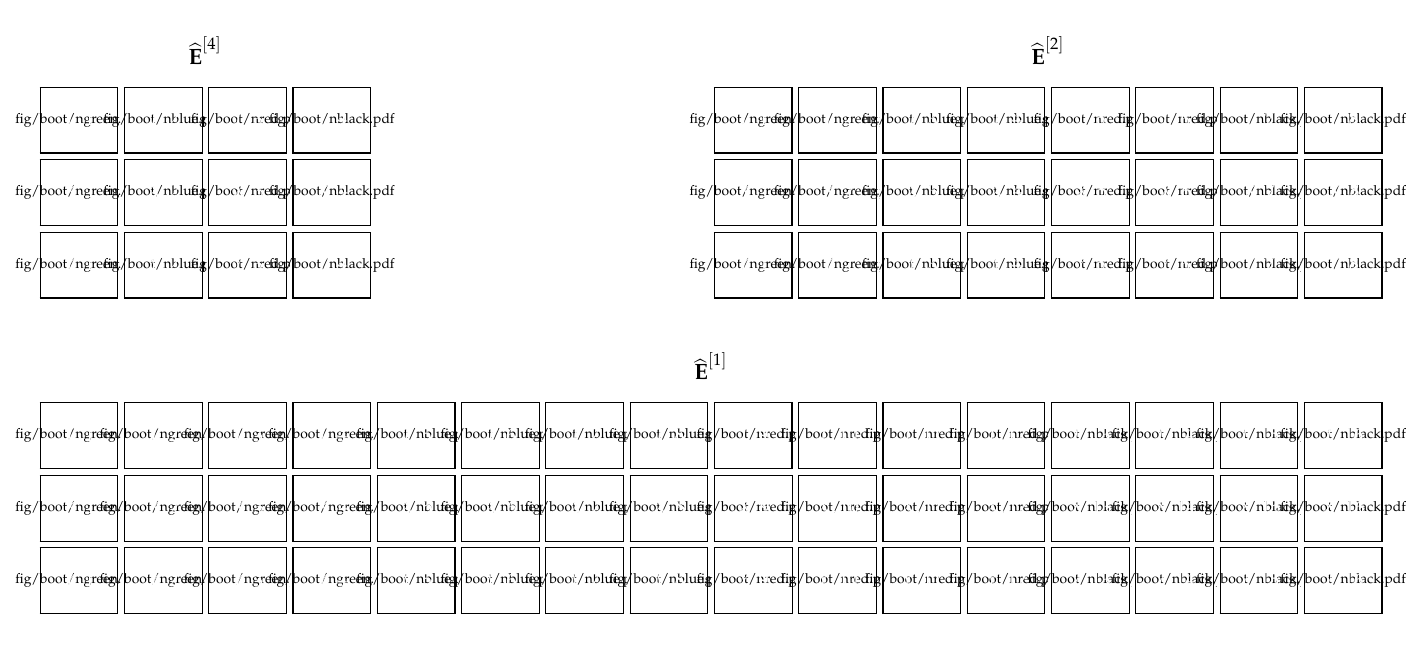
\begin{tikzpicture}
\matrix (e1) [matrix of nodes,row sep=0cm,column sep=0cm, nodes= {rectangle, fill=white, inner sep = 1pt}, label=above:{\footnotesize$\widehat{\textbf{E}}^{[1]}$}]
{
|[label={[font=\scriptsize, text = white, anchor=center]center:{$T,1$}}]|\pgfuseimage{ngreen} & |[label={[font=\scriptsize, text = white, anchor=center]center:{$T,2$}}]|\pgfuseimage{ngreen} & |[label={[font=\scriptsize, text = white, anchor=center]center:{$T,3$}}]|\pgfuseimage{ngreen} & |[label={[font=\scriptsize, text = white, anchor=center]center:{$T,4$}}]|\pgfuseimage{ngreen} & |[label={[font=\scriptsize, text = white, anchor=center]center:{$T,5$}}]|\pgfuseimage{nblue} & |[label={[font=\scriptsize, text = white, anchor=center]center:{$T,6$}}]|\pgfuseimage{nblue}  & |[label={[font=\scriptsize, text = white, anchor=center]center:{$T,7$}}]|\pgfuseimage{nblue} & |[label={[font=\scriptsize, text = white, anchor=center]center:{$T,8$}}]|\pgfuseimage{nblue} & |[label={[font=\scriptsize, text = white, anchor=center]center:{$T,9$}}]|\pgfuseimage{nred} & |[label={[font=\scriptsize, text = white, anchor=center]center:{$T,10$}}]|\pgfuseimage{nred} & |[label={[font=\scriptsize, text = white, anchor=center]center:{$T,11$}}]|\pgfuseimage{nred} & |[label={[font=\scriptsize, text = white, anchor=center]center:{$T,12$}}]|\pgfuseimage{nred} & |[label={[font=\scriptsize, text = white, anchor=center]center:{$T,13$}}]|\pgfuseimage{nblack} & |[label={[font=\scriptsize, text = white, anchor=center]center:{$T,14$}}]|\pgfuseimage{nblack} & |[label={[font=\scriptsize, text = white, anchor=center]center:{$T,15$}}]|\pgfuseimage{nblack} & |[label={[font=\scriptsize, text = white, anchor=center]center:{$T,16$}}]|\pgfuseimage{nblack}\\
|[label={[font=\scriptsize, text = white, anchor=center]center:{$X,1$}}]|\pgfuseimage{ngreen} & |[label={[font=\scriptsize, text = white, anchor=center]center:{$X,2$}}]|\pgfuseimage{ngreen} & |[label={[font=\scriptsize, text = white, anchor=center]center:{$X,3$}}]|\pgfuseimage{ngreen} & |[label={[font=\scriptsize, text = white, anchor=center]center:{$X,4$}}]|\pgfuseimage{ngreen} & |[label={[font=\scriptsize, text = white, anchor=center]center:{$X,5$}}]|\pgfuseimage{nblue} & |[label={[font=\scriptsize, text = white, anchor=center]center:{$X,6$}}]|\pgfuseimage{nblue}  & |[label={[font=\scriptsize, text = white, anchor=center]center:{$X,7$}}]|\pgfuseimage{nblue} & |[label={[font=\scriptsize, text = white, anchor=center]center:{$X,8$}}]|\pgfuseimage{nblue} & |[label={[font=\scriptsize, text = white, anchor=center]center:{$X,9$}}]|\pgfuseimage{nred} & |[label={[font=\scriptsize, text = white, anchor=center]center:{$X,10$}}]|\pgfuseimage{nred} & |[label={[font=\scriptsize, text = white, anchor=center]center:{$X,11$}}]|\pgfuseimage{nred} & |[label={[font=\scriptsize, text = white, anchor=center]center:{$X,12$}}]|\pgfuseimage{nred} & |[label={[font=\scriptsize, text = white, anchor=center]center:{$X,13$}}]|\pgfuseimage{nblack} & |[label={[font=\scriptsize, text = white, anchor=center]center:{$X,14$}}]|\pgfuseimage{nblack} & |[label={[font=\scriptsize, text = white, anchor=center]center:{$X,15$}}]|\pgfuseimage{nblack} & |[label={[font=\scriptsize, text = white, anchor=center]center:{$X,16$}}]|\pgfuseimage{nblack}\\
|[label={[font=\scriptsize, text = white, anchor=center]center:{$Y,1$}}]|\pgfuseimage{ngreen} & |[label={[font=\scriptsize, text = white, anchor=center]center:{$Y,2$}}]|\pgfuseimage{ngreen} & |[label={[font=\scriptsize, text = white, anchor=center]center:{$Y,3$}}]|\pgfuseimage{ngreen} & |[label={[font=\scriptsize, text = white, anchor=center]center:{$Y,4$}}]|\pgfuseimage{ngreen} & |[label={[font=\scriptsize, text = white, anchor=center]center:{$Y,5$}}]|\pgfuseimage{nblue} & |[label={[font=\scriptsize, text = white, anchor=center]center:{$Y,6$}}]|\pgfuseimage{nblue}  & |[label={[font=\scriptsize, text = white, anchor=center]center:{$Y,7$}}]|\pgfuseimage{nblue} & |[label={[font=\scriptsize, text = white, anchor=center]center:{$Y,8$}}]|\pgfuseimage{nblue} & |[label={[font=\scriptsize, text = white, anchor=center]center:{$Y,9$}}]|\pgfuseimage{nred} & |[label={[font=\scriptsize, text = white, anchor=center]center:{$Y,10$}}]|\pgfuseimage{nred} & |[label={[font=\scriptsize, text = white, anchor=center]center:{$Y,11$}}]|\pgfuseimage{nred} & |[label={[font=\scriptsize, text = white, anchor=center]center:{$Y,12$}}]|\pgfuseimage{nred} & |[label={[font=\scriptsize, text = white, anchor=center]center:{$Y,13$}}]|\pgfuseimage{nblack} & |[label={[font=\scriptsize, text = white, anchor=center]center:{$Y,14$}}]|\pgfuseimage{nblack} & |[label={[font=\scriptsize, text = white, anchor=center]center:{$Y,15$}}]|\pgfuseimage{nblack} & |[label={[font=\scriptsize, text = white, anchor=center]center:{$Y,16$}}]|\pgfuseimage{nblack}\\
};

\matrix (ek) [above= 10mm of e1.north east,
       anchor=south east, matrix of nodes,row sep=0cm,column sep=0cm, nodes= {rectangle, fill=white, inner sep = 1pt}, label=above:{\footnotesize$\widehat{\textbf{E}}^{[2]}$}]
{
|[label={[font=\scriptsize, text = white, anchor=center]center:{$T,1$}}]|\pgfuseimage{ngreen} & |[label={[font=\scriptsize, text = white, anchor=center]center:{$T,2$}}]|\pgfuseimage{ngreen} & |[label={[font=\scriptsize, text = white, anchor=center]center:{$T,3$}}]|\pgfuseimage{nblue} & |[label={[font=\scriptsize, text = white, anchor=center]center:{$T,4$}}]|\pgfuseimage{nblue} & |[label={[font=\scriptsize, text = white, anchor=center]center:{$T,5$}}]|\pgfuseimage{nred} & |[label={[font=\scriptsize, text = white, anchor=center]center:{$T,6$}}]|\pgfuseimage{nred} & |[label={[font=\scriptsize, text = white, anchor=center]center:{$T,7$}}]|\pgfuseimage{nblack} & |[label={[font=\scriptsize, text = white, anchor=center]center:{$T,8$}}]|\pgfuseimage{nblack}\\
|[label={[font=\scriptsize, text = white, anchor=center]center:{$X,1$}}]|\pgfuseimage{ngreen} & |[label={[font=\scriptsize, text = white, anchor=center]center:{$X,2$}}]|\pgfuseimage{ngreen} & |[label={[font=\scriptsize, text = white, anchor=center]center:{$X,3$}}]|\pgfuseimage{nblue} & |[label={[font=\scriptsize, text = white, anchor=center]center:{$X,4$}}]|\pgfuseimage{nblue} & |[label={[font=\scriptsize, text = white, anchor=center]center:{$X,5$}}]|\pgfuseimage{nred} & |[label={[font=\scriptsize, text = white, anchor=center]center:{$X,6$}}]|\pgfuseimage{nred} & |[label={[font=\scriptsize, text = white, anchor=center]center:{$X,7$}}]|\pgfuseimage{nblack} & |[label={[font=\scriptsize, text = white, anchor=center]center:{$X,8$}}]|\pgfuseimage{nblack}\\
|[label={[font=\scriptsize, text = white, anchor=center]center:{$Y,1$}}]|\pgfuseimage{ngreen} & |[label={[font=\scriptsize, text = white, anchor=center]center:{$Y,2$}}]|\pgfuseimage{ngreen} & |[label={[font=\scriptsize, text = white, anchor=center]center:{$Y,3$}}]|\pgfuseimage{nblue} & |[label={[font=\scriptsize, text = white, anchor=center]center:{$Y,4$}}]|\pgfuseimage{nblue} & |[label={[font=\scriptsize, text = white, anchor=center]center:{$Y,5$}}]|\pgfuseimage{nred} & |[label={[font=\scriptsize, text = white, anchor=center]center:{$Y,6$}}]|\pgfuseimage{nred} & |[label={[font=\scriptsize, text = white, anchor=center]center:{$Y,7$}}]|\pgfuseimage{nblack} & |[label={[font=\scriptsize, text = white, anchor=center]center:{$Y,8$}}]|\pgfuseimage{nblack}\\
};

\matrix (em) [above= 10mm of e1.north west,
       anchor=south west, matrix of nodes,row sep=0cm,column sep=0cm, nodes= {rectangle, fill=white, inner sep = 1pt}, label=above:{\footnotesize$\widehat{\textbf{E}}^{[4]}$}]
{
|[label={[font=\scriptsize, text = white, anchor=center]center:{$T,1$}}]|\pgfuseimage{ngreen} & |[label={[font=\scriptsize, text = white, anchor=center]center:{$T,2$}}]|\pgfuseimage{nblue} & |[label={[font=\scriptsize, text = white, anchor=center]center:{$T,3$}}]|\pgfuseimage{nred} & |[label={[font=\scriptsize, text = white, anchor=center]center:{$T,4$}}]|\pgfuseimage{nblack}\\
|[label={[font=\scriptsize, text = white, anchor=center]center:{$X,1$}}]|\pgfuseimage{ngreen} & |[label={[font=\scriptsize, text = white, anchor=center]center:{$X,2$}}]|\pgfuseimage{nblue} & |[label={[font=\scriptsize, text = white, anchor=center]center:{$X,3$}}]|\pgfuseimage{nred} & |[label={[font=\scriptsize, text = white, anchor=center]center:{$X,4$}}]|\pgfuseimage{nblack}\\
|[label={[font=\scriptsize, text = white, anchor=center]center:{$Y,1$}}]|\pgfuseimage{ngreen} & |[label={[font=\scriptsize, text = white, anchor=center]center:{$Y,2$}}]|\pgfuseimage{nblue} & |[label={[font=\scriptsize, text = white, anchor=center]center:{$Y,3$}}]|\pgfuseimage{nred} & |[label={[font=\scriptsize, text = white, anchor=center]center:{$Y,4$}}]|\pgfuseimage{nblack}\\
};
\end{tikzpicture}
	\caption{Example of residual matrices for figure 3 with 4 years of data ($N=4$): the green color corresponds to the first year, the blue to the second year, the red to the third year and the black to the fourth year.}
	\label{fig:res_boot}
\end{figure}


An important issue is how to generate base forecasts' samples that preserve cross-temporal relationships. We suggest the cross-temporal joint (block) bootstrap (\textbf{ctjb}) to solve this issue. The approach involves sampling from the most temporally aggregated level ($m$) while maintaining the cross-sectional structure, and using the most temporally aggregated level to determine the samples' indices for the other levels.

Let $\widehat{\Evet}^{[k]}$ be the $(n \times T/k)$ matrix of the in-sample residuals for $k \in \mathcal{K}$. The Figure \ref{fig:res_boot} provides a visualization of these matrices and how they are related to each other for the example in Figure \ref{fig:hierS}. It is assumed that the residuals cover 4 years ($N=4$): the green color corresponds to the first year, the blue to the second year, and so on. Furthermore, let $\mathcal{M}_i$ be the model used to calculate the base forecasts and in-sample residuals for the $i$-th series. In this work, we assume $\mathcal{M}_i$ to be a univariate model, however nothing prevents the use of multivariate models perhaps for different temporal levels or for groups of historical series. Assuming $H = 1$, $\tau$ is a random draw with replacement from $1,\dots, N$ and the $\ell^{th}$ bootstrap incoherent sample is
$$
\widehat{\xvet}_{i,\ell}^{[k]} = f_i\left(\mathcal{M}_i, \widehat{\evet}_{i}^{[k]}\right)
$$
where $f_i(\cdot)$ depend on the fitted univariate model $\mathcal{M}_i$. That is, $\widehat{\xvet}_{i,l}^{[k]}$ is a sample path simulated for the $i$-th series with error approximated by the corresponding block bootstrapped sample residual $\widehat{\evet}_{i}^{[k]}$, the $i$-th row of
	$$
	\widehat{\Evet}^{[k]}_{\tau} = \begin{bmatrix}
		\widehat{e}^{[k]}_{1,M_k(\tau-1)+1} & \dots & \widehat{e}^{[k]}_{1,M_k\tau} \\
		\vdots & \ddots & \vdots \\
		\widehat{e}^{[k]}_{n,M_k(\tau-1)+1} & \dots & \widehat{e}^{[k]}_{n,M_k\tau} \
	\end{bmatrix},
	$$
	where $\widehat{\Evet}_{\tau} = \begin{bmatrix}
		\widehat{\evet}^{[m]}_\tau & \widehat{\Evet}^{[k_{p-1}]}_{\tau} & \dots &\widehat{\Evet}^{[1]}_{\tau}
	\end{bmatrix}$ is a $[n \times (k^\ast + m)]$ matrix where $\widehat{\evet}^{[m]}_\tau$ is the $\tau$-th column of $\widehat{\Evet}^{[m]}$ and $\widehat{\Evet}^{[k]}_{\tau}$ is the $(n \times M_k)$ matrix formed by columns $M_k(\tau-1)+1,\dots, M_k \tau$ of $\widehat{\Evet}^{[k]}$. 	Figure \ref{fig:ct_boot} shows the component of $\widehat{\Evet}_{\tau} = \begin{bmatrix}
		\widehat{\evet}^{[4]}_\tau & \widehat{\Evet}^{[2]}_{\tau}&\widehat{\Evet}^{[1]}_{\tau}
	\end{bmatrix}$ for the quarterly cross-temporal hierarchy in Figure \ref{fig:hierS}.

\begin{figure}[!htb]
\centering
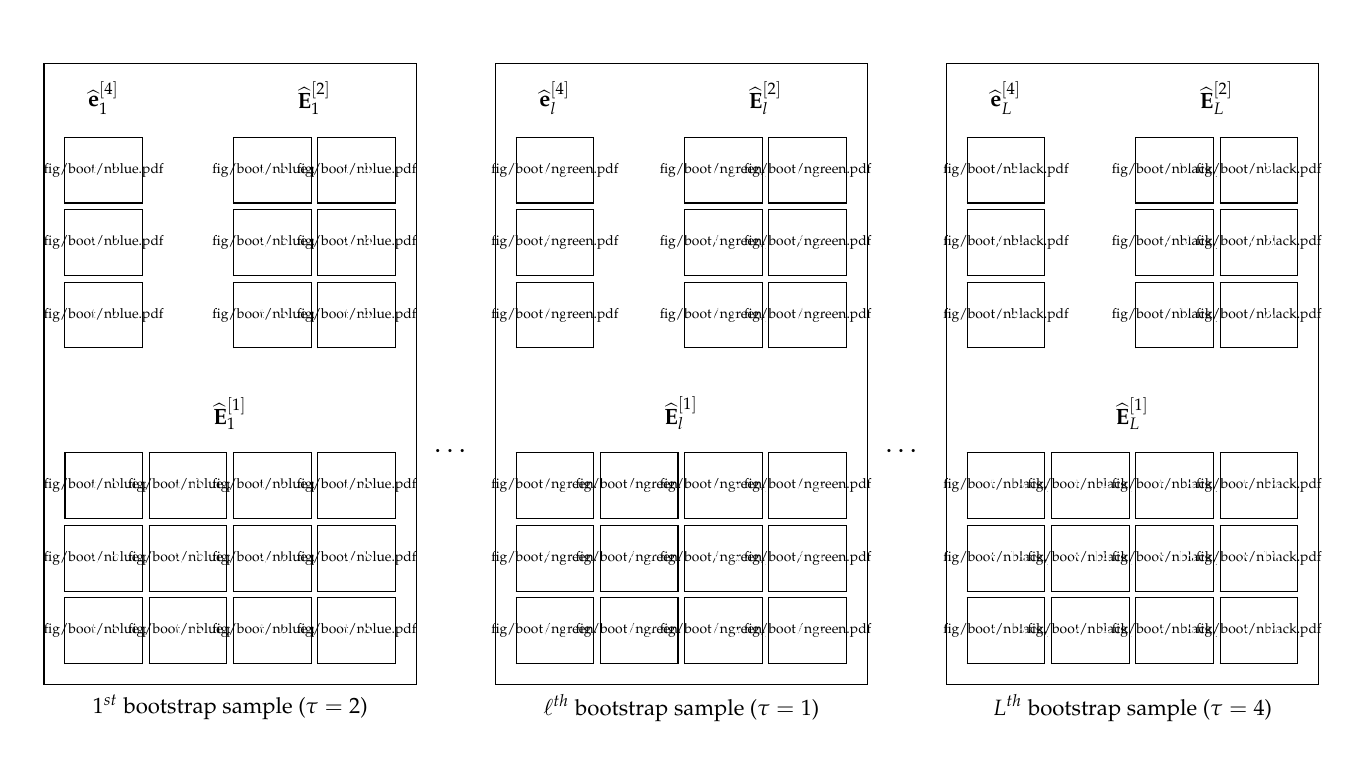
\begin{tikzpicture}
\matrix (e1) [matrix of nodes,row sep=0cm,column sep=0cm, nodes= {rectangle, fill=white, inner sep = 1pt}, label={[name=labe1] above:{\footnotesize$\widehat{\textbf{E}}_1^{[1]}$}}]
{
|[label={[font=\scriptsize, text = white, anchor=center]center:{$T,5$}}]|\pgfuseimage{nblue} & |[label={[font=\scriptsize, text = white, anchor=center]center:{$T,6$}}]|\pgfuseimage{nblue} & |[label={[font=\scriptsize, text = white, anchor=center]center:{$T,7$}}]|\pgfuseimage{nblue} & |[label={[font=\scriptsize, text = white, anchor=center]center:{$T,8$}}]|\pgfuseimage{nblue}\\
|[label={[font=\scriptsize, text = white, anchor=center]center:{$X,5$}}]|\pgfuseimage{nblue} & |[label={[font=\scriptsize, text = white, anchor=center]center:{$X,6$}}]|\pgfuseimage{nblue} & |[label={[font=\scriptsize, text = white, anchor=center]center:{$X,7$}}]|\pgfuseimage{nblue} & |[label={[font=\scriptsize, text = white, anchor=center]center:{$X,8$}}]|\pgfuseimage{nblue}\\
|[label={[font=\scriptsize, text = white, anchor=center]center:{$Y,5$}}]|\pgfuseimage{nblue} & |[label={[font=\scriptsize, text = white, anchor=center]center:{$Y,6$}}]|\pgfuseimage{nblue} & |[label={[font=\scriptsize, text = white, anchor=center]center:{$Y,7$}}]|\pgfuseimage{nblue} & |[label={[font=\scriptsize, text = white, anchor=center]center:{$Y,8$}}]|\pgfuseimage{nblue}\\
};

\matrix (ek) [above= 10mm of e1.north east,
       anchor=south east, matrix of nodes,row sep=0cm,column sep=0cm, nodes= {rectangle, fill=white, inner sep = 1pt}, label={[name=labek] above:{\footnotesize$\widehat{\textbf{E}}_1^{[2]}$}}]
{
|[label={[font=\scriptsize, text = white, anchor=center]center:{$T,3$}}]|\pgfuseimage{nblue} & |[label={[font=\scriptsize, text = white, anchor=center]center:{$T,4$}}]|\pgfuseimage{nblue} \\
|[label={[font=\scriptsize, text = white, anchor=center]center:{$X,3$}}]|\pgfuseimage{nblue} & |[label={[font=\scriptsize, text = white, anchor=center]center:{$X,4$}}]|\pgfuseimage{nblue} \\
|[label={[font=\scriptsize, text = white, anchor=center]center:{$Y,3$}}]|\pgfuseimage{nblue} & |[label={[font=\scriptsize, text = white, anchor=center]center:{$Y,4$}}]|\pgfuseimage{nblue} \\
};

\matrix (em) [above= 10mm of e1.north west,
       anchor=south west, matrix of nodes,row sep=0cm,column sep=0cm, nodes= {rectangle, fill=white, inner sep = 1pt}, label={[name=labem] above:{\footnotesize$\widehat{\textbf{e}}_1^{[4]}$}}]
{
|[label={[font=\scriptsize, text = white, anchor=center]center:{$T,2$}}]|\pgfuseimage{nblue} \\
|[label={[font=\scriptsize, text = white, anchor=center]center:{$X,2$}}]|\pgfuseimage{nblue} \\
|[label={[font=\scriptsize, text = white, anchor=center]center:{$Y,2$}}]|\pgfuseimage{nblue} \\
};


\node[right= 2mm of e1.north east,
       anchor=north west] {$\dots$};
\matrix (e1_l) [right= 12mm of e1.north east,
       anchor=north west, matrix of nodes,row sep=0cm,column sep=0cm, nodes= {rectangle, fill=white, inner sep = 1pt}, label={[name=labe1l] above:{\footnotesize$\widehat{\textbf{E}}_l^{[1]}$}}]
{
|[label={[font=\scriptsize, text = white, anchor=center]center:{$T,1$}}]|\pgfuseimage{ngreen} & |[label={[font=\scriptsize, text = white, anchor=center]center:{$T,2$}}]|\pgfuseimage{ngreen} & |[label={[font=\scriptsize, text = white, anchor=center]center:{$T,3$}}]|\pgfuseimage{ngreen} & |[label={[font=\scriptsize, text = white, anchor=center]center:{$T,4$}}]|\pgfuseimage{ngreen}\\
|[label={[font=\scriptsize, text = white, anchor=center]center:{$X,1$}}]|\pgfuseimage{ngreen} & |[label={[font=\scriptsize, text = white, anchor=center]center:{$X,2$}}]|\pgfuseimage{ngreen} & |[label={[font=\scriptsize, text = white, anchor=center]center:{$X,3$}}]|\pgfuseimage{ngreen} & |[label={[font=\scriptsize, text = white, anchor=center]center:{$X,4$}}]|\pgfuseimage{ngreen}\\
|[label={[font=\scriptsize, text = white, anchor=center]center:{$Y,1$}}]|\pgfuseimage{ngreen} & |[label={[font=\scriptsize, text = white, anchor=center]center:{$Y,2$}}]|\pgfuseimage{ngreen} & |[label={[font=\scriptsize, text = white, anchor=center]center:{$Y,3$}}]|\pgfuseimage{ngreen} & |[label={[font=\scriptsize, text = white, anchor=center]center:{$Y,4$}}]|\pgfuseimage{ngreen}\\
};

\matrix (ek_l) [above= 10mm of e1_l.north east,
       anchor=south east, matrix of nodes,row sep=0cm,column sep=0cm, nodes= {rectangle, fill=white, inner sep = 1pt}, label={[name=labekl] above:{\footnotesize$\widehat{\textbf{E}}_l^{[2]}$}}]
{
|[label={[font=\scriptsize, text = white, anchor=center]center:{$T,1$}}]|\pgfuseimage{ngreen} & |[label={[font=\scriptsize, text = white, anchor=center]center:{$T,2$}}]|\pgfuseimage{ngreen} \\
|[label={[font=\scriptsize, text = white, anchor=center]center:{$X,1$}}]|\pgfuseimage{ngreen} & |[label={[font=\scriptsize, text = white, anchor=center]center:{$X,2$}}]|\pgfuseimage{ngreen} \\
|[label={[font=\scriptsize, text = white, anchor=center]center:{$Y,1$}}]|\pgfuseimage{ngreen} & |[label={[font=\scriptsize, text = white, anchor=center]center:{$Y,2$}}]|\pgfuseimage{ngreen} \\
};

\matrix (em_l) [above= 10mm of e1_l.north west,
       anchor=south west, matrix of nodes,row sep=0cm,column sep=0cm, nodes= {rectangle, fill=white, inner sep = 1pt}, label={[name=labeml] above:{\footnotesize$\widehat{\textbf{e}}_l^{[4]}$}}]
{
|[label={[font=\scriptsize, text = white, anchor=center]center:{$T,1$}}]|\pgfuseimage{ngreen} \\
|[label={[font=\scriptsize, text = white, anchor=center]center:{$X,1$}}]|\pgfuseimage{ngreen} \\
|[label={[font=\scriptsize, text = white, anchor=center]center:{$Y,1$}}]|\pgfuseimage{ngreen} \\
};

\node[right= 2mm of e1_l.north east,
       anchor=north west] {$\dots$};
\matrix (e1_L) [right= 12mm of e1_l.north east,
       anchor=north west, matrix of nodes,row sep=0cm,column sep=0cm, nodes= {rectangle, fill=white, inner sep = 1pt}, label={[name=labe1L] above:{\footnotesize$\widehat{\textbf{E}}_L^{[1]}$}}]
{
|[label={[font=\scriptsize, text = white, anchor=center]center:{$T,13$}}]|\pgfuseimage{nblack} & |[label={[font=\scriptsize, text = white, anchor=center]center:{$T,14$}}]|\pgfuseimage{nblack} & |[label={[font=\scriptsize, text = white, anchor=center]center:{$T,15$}}]|\pgfuseimage{nblack} & |[label={[font=\scriptsize, text = white, anchor=center]center:{$T,16$}}]|\pgfuseimage{nblack}\\
|[label={[font=\scriptsize, text = white, anchor=center]center:{$X,13$}}]|\pgfuseimage{nblack} & |[label={[font=\scriptsize, text = white, anchor=center]center:{$X,14$}}]|\pgfuseimage{nblack} & |[label={[font=\scriptsize, text = white, anchor=center]center:{$X,15$}}]|\pgfuseimage{nblack} & |[label={[font=\scriptsize, text = white, anchor=center]center:{$X,16$}}]|\pgfuseimage{nblack}\\
|[label={[font=\scriptsize, text = white, anchor=center]center:{$Y,13$}}]|\pgfuseimage{nblack} & |[label={[font=\scriptsize, text = white, anchor=center]center:{$Y,14$}}]|\pgfuseimage{nblack} & |[label={[font=\scriptsize, text = white, anchor=center]center:{$Y,15$}}]|\pgfuseimage{nblack} & |[label={[font=\scriptsize, text = white, anchor=center]center:{$Y,16$}}]|\pgfuseimage{nblack}\\
};


\matrix (ek_L) [above= 10mm of e1_L.north east,
       anchor=south east, matrix of nodes,row sep=0cm,column sep=0cm, nodes= {rectangle, fill=white, inner sep = 1pt}, label={[name=labekL] above:{\footnotesize$\widehat{\textbf{E}}_L^{[2]}$}}]
{
|[label={[font=\scriptsize, text = white, anchor=center]center:{$T,7$}}]|\pgfuseimage{nblack} & |[label={[font=\scriptsize, text = white, anchor=center]center:{$T,8$}}]|\pgfuseimage{nblack} \\
|[label={[font=\scriptsize, text = white, anchor=center]center:{$X,7$}}]|\pgfuseimage{nblack} & |[label={[font=\scriptsize, text = white, anchor=center]center:{$X,8$}}]|\pgfuseimage{nblack} \\
|[label={[font=\scriptsize, text = white, anchor=center]center:{$Y,7$}}]|\pgfuseimage{nblack} & |[label={[font=\scriptsize, text = white, anchor=center]center:{$Y,8$}}]|\pgfuseimage{nblack} \\
};

\matrix (em_L) [above= 10mm of e1_L.north west,
       anchor=south west, matrix of nodes,row sep=0cm,column sep=0cm, nodes= {rectangle, fill=white, inner sep = 1pt}, label={[name=labemL] above:{\footnotesize$\widehat{\textbf{e}}_L^{[4]}$}}]
{
|[label={[font=\scriptsize, text = white, anchor=center]center:{$T,4$}}]|\pgfuseimage{nblack} \\
|[label={[font=\scriptsize, text = white, anchor=center]center:{$X,4$}}]|\pgfuseimage{nblack} \\
|[label={[font=\scriptsize, text = white, anchor=center]center:{$Y,4$}}]|\pgfuseimage{nblack} \\
};


\node[draw,inner sep=1mm,label={[name = boot1n] below:{\footnotesize$1^{st}$ bootstrap sample ($\tau = 2$)}},fit=(e1) (ek) (em) (labek) (labe1) (labem)] (boot1) {};
\node[draw,inner sep=1mm,label={[name = boot2n] below:{\footnotesize$\ell^{th}$ bootstrap sample ($\tau = 1$)}},fit=(e1_l) (ek_l) (em_l) (labekl) (labe1l) (labeml)] (boot2) {};
\node[draw,inner sep=1mm,label={[name = boot3n] below:{\footnotesize$L^{th}$ bootstrap sample ($\tau = 4$)}},fit=(e1_L) (ek_L) (em_L) (labekL) (labe1L) (labemL)] (boot3) {};

\node[inner sep=2mm,label=above:{},fit=(boot3) (boot2) (boot1) (boot3n) (boot2n) (boot1n)] {};
\end{tikzpicture}

\caption{Example of bootstrapped residuals for the cross-temporal hierarchy of Figure \ref{fig:hierS} and using the residuals in Figure \ref{fig:res_boot}.}
\label{fig:ct_boot}
\end{figure}


One of the main advantages of the cross-temporal joint bootstrap is that it allows us to accurately account for the dependence between the different levels of temporal aggregation and not only the cross-sectional dependencies. By sampling residuals from the most temporally aggregated level and using it to determine the indices for the other levels, we can ensure that the bootstrap sample reflects the underlying data distribution. Additionally, the cross-temporal joint bootstrap is easy to implement in \textsf{R} \citep{rcoreteam2022} using the package \texttt{forecast} \citep{Rforecast} for many forecasting models, making it a practical and efficient tool. Furthermore, this approach is easily scalable in order to utilize multiple computing power simultaneously for each cross-sectional series. This can be especially useful when dealing with large datasets or when trying to speed up the analysis process.

\subsection{Parametric framework: Gaussian reconciliation}\label{ssec:prob_pf}
It is possible to obtain a reconciled probabilistic forecast analytically for some parametric distributions, such as the multivariate normal \citep{panagiotelis2023, wickramasuriya2021b, corani2021, eckert2021}. In the cross-sectional framework, \cite{panagiotelis2023} show that, starting from an elliptical distribution for the base forecasts, the reconciled forecast distribution is also elliptical. Then this is valid for the multivariate normal that is an elliptical distribution characterized by its first two moments. Using the matrix notation in Section \ref{sec:not}, we may extend this results to the cross-temporal case.
%Therefore, fixed $H = 1$, if the base forecasts distribution is $\mathcal{N}(\widehat{\xvet}, \Omegavet)$, then the reconciled forecasts distribution is $\mathcal{N}(\widetilde{\xvet}, \widetilde{\Omegavet})$, where
To obtain a reconciled forecast using the multivariate normal distribution for given  $H = 1$, we start with a base forecast distributed as $\mathcal{N}(\widehat{\xvet}, \Sigmavet)$, where $\widehat{\xvet}_h$ is the mean vector and $\Sigmavet$ is the covariance matrix of the base forecasts. The reconciled forecast distribution is then given by $\mathcal{N}(\widetilde{\xvet}, \widetilde{\Omegavet})$, where
\begin{equation}\label{eq:meanvar}
	\widetilde{\xvet} = \Mvet\widehat{\xvet} \quad \mbox{and} \quad \widetilde{\Omegavet} = \Mvet \Sigmavet \Mvet',
\end{equation}
where $\Mvet$ is the projection matrix defined in equation (\ref{eq:Mvet}).
Note that if we assume that $\Sigmavet = \Omegavet_{ct}$, then the covariance matrix equation (\ref{eq:meanvar}) simplifies to $\widetilde{\Omegavet} = \Mvet \Omegavet_{ct}$.
%The covariance matrix $\Sigmavet$ is a key component of the reconciled forecast and it is important to carefully consider how it is calculated and deserves special attention. Accurately estimating the covariance matrix is important for several reasons. First, it allows us to quantify the uncertainty associated with our forecasts, which is crucial for decision-making. Second, the covariance matrix plays a key role in many statistical models and algorithms, so an incorrect estimate can lead to biased or unreliable results.
In the cross-temporal case, accurately estimating the covariance matrix $\Sigmavet$ can be difficult because we need to consider simultaneously both the temporal and cross-sectional structure. This requires many parameters to be estimated, which can be challenging in practice. Additionally, using in-sample residuals to estimate the cross-temporal correlation structure can lead to an incorrect estimate of the covariance matrix, as the residuals may not accurately capture the true correlation structure. These challenges will be explored in more depth in the following sections.

Focusing on the computational aspect, we can take several steps to reduce the time required to obtain simulations from the reconciled forecast distribution. For example, it is not necessary to simulate from a normal distribution with a defined covariance matrix for the entire structure when dealing with a genuine hierarchical structure. Instead, we can utilize the properties of elliptical distributions to simulate from the high frequency bottom time series and then to obtain the complete simulation through the $\Svet_{ct}$ matrix. Furthermore, we do not need to calculate the reconciled mean and variance and generate a new sample if we already have a sample from the normal distribution of the base forecasts; we can simply apply the point forecast reconciliation formula (\ref{eq:Mvet}) as outlined in Theorem \ref{thm:rs}, which is still valid for parametric cases. The relationships between base and reconciled forecast distributions and their respective simulations through Theorem \ref{thm:rs} are depicted in Figure \ref{fig:gaussrel}.

\begin{figure}
	\centering
	\begingroup
	\spacingset{0.9}
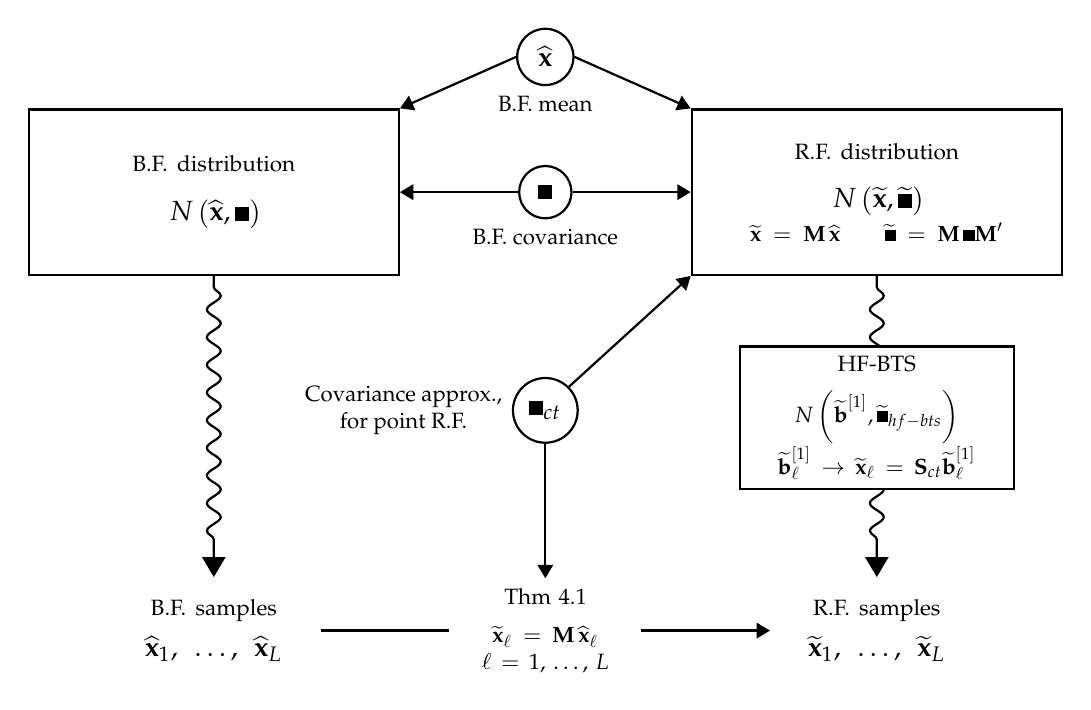
\begin{tikzpicture}

\node[draw, thick, inner sep=1mm, minimum width = 1cm, text width=4.5cm, minimum height = 2.1cm, text centered] (dist) {{\footnotesize R.F. distribution} \\[0.2cm] 
%$\textbf{M} = f(\mathbf{\Omega})$\\[0.2cm] 
$N\left(\widetilde{\textbf{x}}, \widetilde{\mathbf{\Omega}} \right)$\\
{\footnotesize $\widetilde{\textbf{x}} = \textbf{M}\,\widehat{\textbf{x}}\qquad \widetilde{\mathbf{\Omega}} = \textbf{M}\,\mathbf{\Sigma}\textbf{M}'$}};

\node[draw, thick, circle, inner sep=1mm, text width=0.35cm, text centered, minimum width = 0.5cm, minimum height = 0.5cm, left= 1.5cm of dist, label={[align=center, font=\footnotesize]below:{B.F. covariance}}] (cov) {$\mathbf{\Sigma}$};


\node[draw, thick, inner sep=1mm, minimum width = 1cm, text width=4.5cm, minimum height = 2.1cm, text centered, left= 1.5cm of cov] (dist2) {{\footnotesize B.F. distribution} \\[0.2cm] $N\left(\widehat{\textbf{x}}, \mathbf{\Sigma}\right)$};

\node[draw, thick, circle, inner sep=1mm, text width=0.5cm, text centered, minimum width = 0.5cm, minimum height = 0.5cm, below = 2cm of cov, label={[align=center, font=\footnotesize]left:{Covariance approx., \\for point R.F.}}] (covapprx) {$\mathbf{\Omega}_{ct}$};

\node[draw, thick, circle, inner sep=1mm, text width=0.35cm, text centered, minimum width = 0.5cm, minimum height = 0.5cm, above = 1cm of cov, label=below:{\footnotesize B.F. mean}] (mean) {$\widehat{\textbf{x}}$};

\node[inner sep=1mm, minimum width = 1cm, text width=2.5cm, text centered, below= 4cm of dist2] (sim_base) {{\footnotesize B.F. samples} \\[0.1cm] $\widehat{\mathbf{x}}_{1}, \;\dots, \;\widehat{\mathbf{x}}_{L}$};

\node[inner sep=1mm, minimum width = 1cm, text width=2.5cm, text centered, below= 4cm of dist] (sim_reco) {{\footnotesize R.F. samples} \\[0.1cm] $\widetilde{\mathbf{x}}_{1}, \;\dots, \;\widetilde{\mathbf{x}}_{L}$};

\draw[-{Triangle[scale=1]}, decorate, thick] (mean.east) -- (dist.north west);
\draw[-{Triangle[scale=1]}, decorate, thick] (cov) -- (dist);
\draw[-{Triangle[scale=1]}, decorate, thick] (mean.west) -- (dist2.north east);
\draw[-{Triangle[scale=1]}, decorate, thick] (cov) -- (dist2);
\draw[-{Triangle[scale=1]}, decorate, thick] (covapprx.north east) -- (dist.south west);


\path[-{Triangle[scale=1]}, decorate, thick] (sim_base) edge node[ fill=white, anchor=center, pos=0.5,font = \footnotesize, text width = 2.2cm, text centered] (nodemid) {Thm 4.1 \\[0.15cm] $\widetilde{\mathbf{x}}_{\ell} = \textbf{M}\,\widehat{\mathbf{x}}_{\ell}$ \\ $\ell = 1,\, \dots,\, L$} (sim_reco);

\draw[-{Triangle[scale=1]}, decorate, thick] (covapprx.south) -- (nodemid.north);

\draw [-{Triangle[scale=1.5]}, decorate, decoration={snake,pre length=4pt,post length=15pt}, thick, shorten >= 5pt] (dist2) -- (sim_base);

%\draw [-{Triangle[scale=1.5]}, decorate, decoration={snake,pre length=4pt,post length=15pt}, thick, shorten >= 5pt] (dist) -- (sim_reco) node[midway, right, xshift = 0.25cm, font = \footnotesize, text width = 3cm, text centered] {$\widetilde{B}^{[1]}\sim N\left(\widetilde{\textbf{b}}^{[1]}, \widetilde{\mathbf{\Omega}}^{[1]}_{b} \right)$ \\ $\widetilde{\textbf{b}}^{[1]}_{h,1}, \, \dots, \, \widetilde{\textbf{b}}^{[1]}_{h,L}$};

\draw [-{Triangle[scale=1.5]}, decorate, decoration={snake,pre length=4pt,post length=15pt}, thick, shorten >= 5pt] (dist) -- (sim_reco)  node[draw, midway, font = \footnotesize, text width = 3.25cm, text centered, fill = white, yshift = 0.2cm] {HF-BTS\\[0.2cm]$N\left(\widetilde{\textbf{b}}^{[1]}, \widetilde{\mathbf{\Omega}}_{hf-bts} \right)$ \\ $\widetilde{\textbf{b}}^{[1]}_{\ell} \rightarrow \widetilde{\textbf{x}}_{\ell}=\textbf{S}_{ct} \widetilde{\textbf{b}}^{[1]}_{\ell}$} ;

\end{tikzpicture}
	\endgroup
	\caption{Summary diagram of reconciliation in the Gaussian framework, as described in Section \ref{ssec:prob_pf}. The acronyms R.F and B.F. stand for Reconciled Forecasts and Base Forecasts, respectively. HF-BTS stands for High Frequency Bottom Time Series.}
	\label{fig:gaussrel} 
\end{figure}

\section{Shrinkage techniques for cross-temporal covariance matrix estimation}\label{sec:shrtech}
In this section, our focus will be exclusively on the cross-temporal framework. As a result, we will not be including the $ct$ subscript in our discussion at this time in order to simplify the notation.

As the covariance matrix $\Omegavet$ is unknown in practice, a natural estimate is the empirical sample covariance matrix of the base forecasts $\widehat{\Omegavet}$. In the cross-temporal framework this means that we have to estimate $r = \displaystyle\frac{n(k^\ast+m)[n(k^\ast+m)-1]}{2}$ different parameters. A possible solution to estimating a large number of parameters when we have less observations than $r$, is to construct an shrinkage estimator \citep{efron1975a,efron1975,efron1977}. The so called “biased estimation” may improved the quality of the estimated variance-covariance matrix by variance reduction though a convex combination of $\widehat{\Omegavet}$ and a target matrix $\widehat{\Omegavet}_D = \widehat{\Omegavet} \odot \Ivet_{n(k^\ast+m)}$, such that
\begin{equation}\label{eq:global}
\widehat{\Omegavet}_{G} = \lambda \widehat{\Omegavet}_D + (1-\lambda) \widehat{\Omegavet},
\end{equation}
where $\lambda \in [0,1]$ is the shrinkage intensity parameter.
\cite{schafer2005} proposed an unbiased estimator for the shrinkage intensity parameter, which is defined as
$$
\widehat{\lambda}=\frac{\sum_{i \neq j} \widehat{\mathrm{Var}}(\widehat{\sigma}_{i j})}{\sum_{i \neq j} \widehat{\sigma}_{i j}^2},
$$
where $\widehat{\sigma}_{i j}$ is the $i j$-th element of $\widehat{\Omegavet}$. In finite samples, $\widehat{\lambda}$ may exceed unity or even become negative; to avoid over-shrinkage or negative shrinkage, the condition
$$
\widehat{\lambda}^\ast=\max \left[0, \min \left(1, \widehat{\lambda}\right)\right]
$$
is imposed to ensure that the estimated $\lambda$ stays within the range $[0,1]$. According to expression (\ref{eq:global}), there are two possible target matrices: a full matrix ($\lambda=0$), and a diagonal matrix ($\lambda=1$). These matrices are shown in the first column of Figure \ref{fig:shr_grid}. This linear combination, which reduces all elements outside the diagonal to zero, can be referred to as \textit{Global shrinkage} (\textit{G}). $\widehat{\Omegavet}_{G}$ corresponds to the matrix used by the reconciliation approach oct$(shr)$ shown in Section \ref{ssec:oct}. This method allows us to shrink the entire off-diagonal portion of the covariance matrix, effectively reducing its complexity and potentially improving its estimation accuracy.

However, arbitrarily setting the off-diagonal elements to zero when we know that the covariance matrix has a cross-sectional and/or temporal structure would result in information loss. The idea is therefore to estimate a smaller matrix (in terms of dimensions) and then to use the cross-sectional and/or temporal structure to obtain a better estimator for the covariance matrix of the entire system. We consider three different approaches at this purpose.

The first idea is to use both cross-sectional and temporal structure simultaneously. Thus, in general we know that the true covariance matrix can be written as
\begin{equation}
	\label{eq:OmSct}
\Omegavet= \Svet_{ct}\Omegavet_{hf-bts}\Svet_{ct}'
\end{equation}
where $\Omegavet_{hf-bts}$ is the covariance matrix for the bottom time series at aggregation level $k = 1$ (high frequency bottom time series).
Therefore, we can apply the idea of “Stein-type shrinkage" to $\Omegavet_{hf-bts}$ by using the empirical covariance matrix of the high frequency bottom base forecasts $\widehat{\Omegavet}_{hf-bts}$, such that
$$
\widehat{\Omegavet}_{hf-bts, HB} = \lambda \widehat{\Omegavet}_{hf-bts, D} + (1-\lambda) \widehat{\Omegavet}_{hf-bts}
$$
and
\begin{align*}
	\widehat{\Omegavet}_{HB} & = \Svet_{ct}\widehat{\Omegavet}_{hf-bts, HB}\Svet_{ct}'\\
	& = \lambda \Svet_{ct}\widehat{\Omegavet}_{hf-bts, D}\Svet_{ct}'+ (1-\lambda) \Svet_{ct}\widehat{\Omegavet}_{hf-bts}\Svet_{ct}',
\end{align*}
where $\widehat{\Omegavet}_{hf-bts, D} = \Ivet_{n_b m}\odot\widehat{\Omegavet}_{hf-bts, HB}$ is a diagonal matrix, $\lambda$ is the shrinkage parameter that can be estimate using \cite{schafer2005} and $\widehat{\Omegavet}_{HB}$ is the cross-temporal covariance matrix for the complete system (\textit{High frequency Bottom time series shrinkage, HB}).
It is worth noting that when using this approach, the covariance matrix of the reconciliation and the base forecasts will be identical. This means that the reconciliation process does not affect the covariance structure of the forecasts, which is determined only by the covariance matrix of the base forecasts errors. In general, the covariance matrix of the reconciled forecasts is equal to $\Mvet \widehat{\Omegavet}_{HB} \Mvet'$ where $\Mvet = \Svet_{ct}\Gvet$ is the projection matrix. Indeed, it can be shown (see \citealp{panagiotelis2021} for more details) that if $\Mvet$ is a projection matrix (\ref{eq:Mvet}) then $\Mvet\Svet_{ct} = \Svet_{ct}\Gvet\Svet_{ct} = \Svet_{ct}$, and we obtain that
$$
\begin{aligned}
	\Mvet \widehat{\Omegavet}_{HB} \Mvet' & = \Mvet\Svet_{ct}\widehat{\Omegavet}_{hf-bts, HB}\Svet_{ct}'\Mvet' \\
	& = \Svet_{ct}\Gvet\Svet_{ct}\widehat{\Omegavet}_{hf-bts, HB}\Svet_{ct}'\Gvet'\Svet_{ct}' \\
	& = \Svet_{ct}\widehat{\Omegavet}_{hf-bts, HB}\Svet_{ct}' = \widehat{\Omegavet}_{HB}.
\end{aligned}
$$
\begin{figure}[t]
\centering
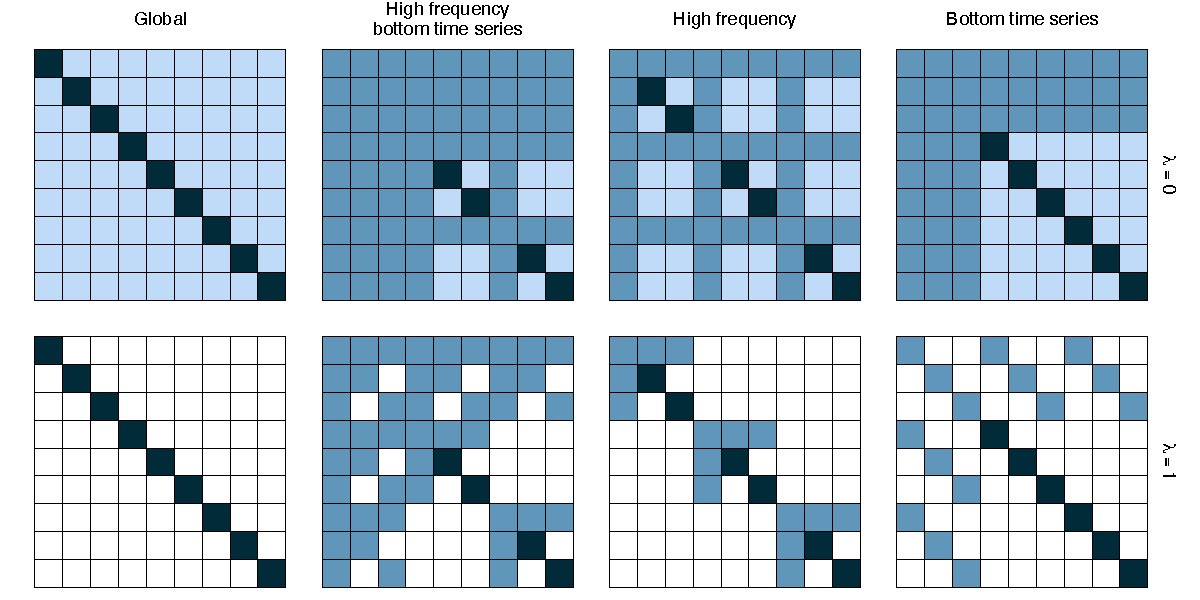
\includegraphics[width = \linewidth]{fig/shr_cov/shr_color.pdf}
\caption{Representation of four types of covariance matrices that can be obtained from the cross-temporal hierarchical structure ($3$ time series and $m = 2$) for two different values of $\lambda\in\{0,1\}$, the shrinkage parameter. The cells that are not modified by shrinkage are colored black, those actively involved in the shrinkage phase are colored light blue, and those derived from and not estimated by the base forecasts errors are colored blue. Additionally, for $\lambda = 1$, the cells corresponding to a zero value are colored white.}
\label{fig:shr_grid}
\end{figure}
However, when working with general linearly constrained multiple time series (where a natural hierarchy representation is not available), we may prefer not to impose the cross-sectional structure. Starting from (\ref{eq:OmSct}), we know that
\begin{align*}
	\Omegavet & = \Svet_{ct}\Omegavet_{hf-bts}\Svet_{ct}'\\
	 & = \left(\Svet_{cs} \otimes \Svet_{te}\right)\Omegavet_{hf-bts}\left(\Svet_{cs} \otimes \Svet_{te}\right)'\\
	 & = \left(\Ivet_n \otimes \Svet_{te}\right)\left(\Svet_{cs} \otimes \Ivet_{m+k^\ast}\right)\Omegavet_{hf-bts}\left(\Svet_{cs} \otimes \Ivet_{m+k^\ast}\right)'\left(\Ivet_n \otimes \Svet_{te}\right)'\\
	 & = \left(\Ivet_n \otimes \Svet_{te}\right)\Omegavet_{hf}\left(\Ivet_n \otimes \Svet_{te}\right)'
\end{align*}
where $\Omegavet_{hf} = \left(\Svet_{cs} \otimes \Ivet_{m+k^\ast}\right)\Omegavet_{hf-bts}\left(\Svet_{cs} \otimes \Ivet_{m+k^\ast}\right)'$ is the covariance matrix related to all the high frequency time series and $\Svet_{ct} = \Svet_{cs} \otimes \Svet_{te} = \left(\Ivet_n \otimes \Svet_{te}\right)\left(\Svet_{cs} \otimes \Ivet_{m+k^\ast}\right)$. We can estimate the matrix $\Omegavet_{hf}$ using the high frequency base forecasts $\widehat{\Omegavet}_{hf}$. Therefore,
$$
\widehat{\Omegavet}_{hf, H} = \lambda \widehat{\Omegavet}_{hf, D} + (1-\lambda) \widehat{\Omegavet}_{hf}
$$
and
\begin{align*}
	\widehat{\Omegavet}_{H} & = (\Ivet_{n} \otimes \Svet_{te})\widehat{\Omegavet}_{hf, H} (\Ivet_{n} \otimes \Svet_{te})'\\
	& = \lambda (\Ivet_{n} \otimes \Svet_{te})\widehat{\Omegavet}_{hf, D}(\Ivet_{n} \otimes \Svet_{te})' + (1-\lambda) (\Ivet_{n} \otimes \Svet_{te})\widehat{\Omegavet}_{hf}(\Ivet_{n} \otimes \Svet_{te})'
\end{align*}
where $\widehat{\Omegavet}_{hf, D} = \Ivet_{nm}\odot\widehat{\Omegavet}_{hf, HB}$ is a diagonal matrix, and $\widehat{\Omegavet}_{H}$ is the cross-temporal covariance matrix for the complete system (\textit{High frequency shrinkage, H}).

\begin{figure}[t]
\centering
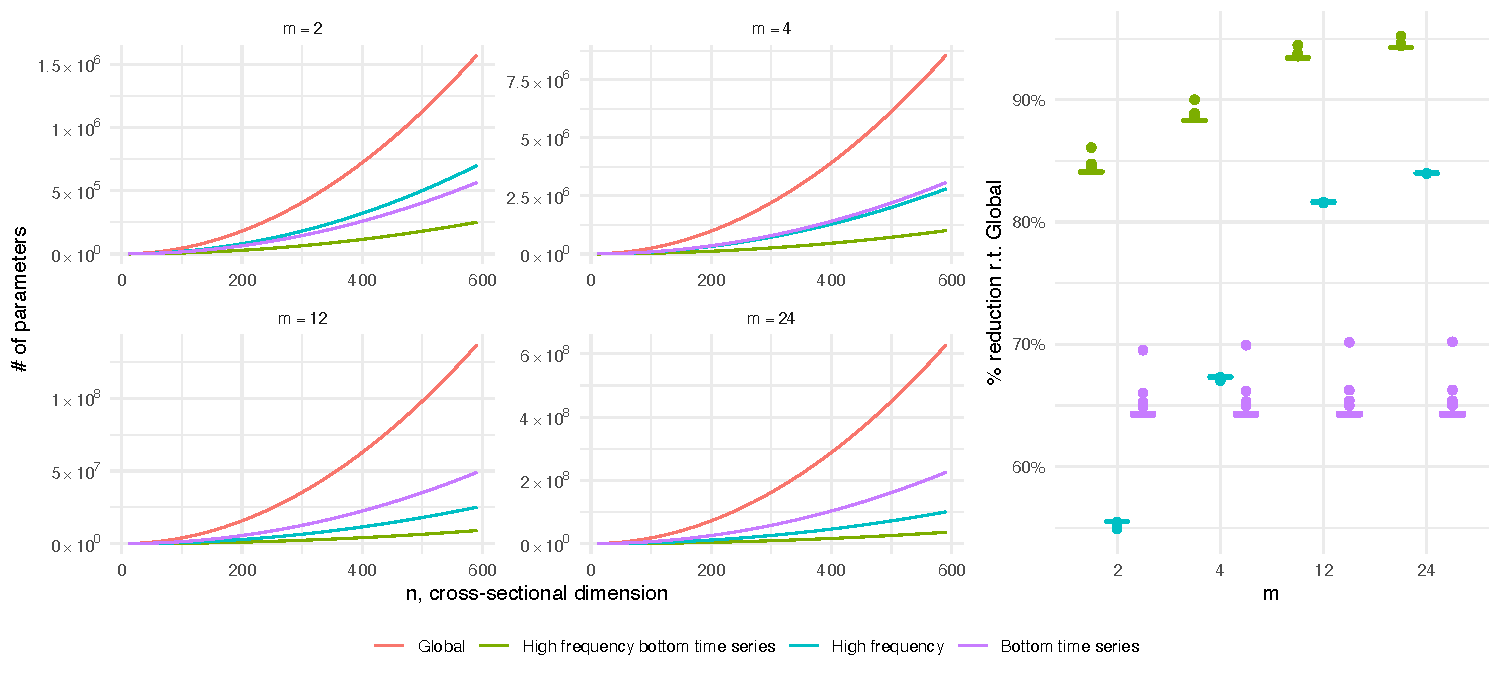
\includegraphics[width = \linewidth]{fig/shr_cov/parameters.pdf}
\caption{The four graphs on the left represent the number of different parameters in the covariance matrix for the various approaches presented for different values of $m$ and $n$ (with $n_b$, the number of bottom time series, is about $60\%$ of the total). On the right, we have the boxplot of the percentage reduction in the number of parameters compared to the global approach.}
\label{fig:num_param}
\end{figure}

Finally, we can impose only the cross-sectional structure. We know that \begin{align*}
	\Omegavet & = \Svet_{ct}\Omegavet_{hf-bts}\Svet_{ct}'\\
	 & = \left(\Svet_{cs} \otimes \Svet_{te}\right)\Omegavet_{hf-bts}\left(\Svet_{cs} \otimes \Svet_{te}\right)'\\
	 & = \left(\Svet_{cs} \otimes \Ivet_{m+k^\ast}\right)\left(\Ivet_n \otimes \Svet_{te}\right)\Omegavet_{hf-bts}\left(\Ivet_n \otimes \Svet_{te}\right)'\left(\Ivet_n \otimes \Svet_{te}\right)'\\
	 & = \left(\Svet_{cs} \otimes \Ivet_{m+k^\ast}\right)\Omegavet_{bts}\left(\Svet_{cs} \otimes \Ivet_{m+k^\ast}\right)'
\end{align*}
where $\Omegavet_{bts} = \left(\Ivet_n \otimes \Svet_{te}\right)\Omegavet_{hf-bts}\left(\Ivet_n \otimes \Svet_{te}\right)'$ is the covariance matrix related to bottom time series at any temporal aggregation, and $\Svet_{ct} = \Svet_{cs} \otimes \Svet_{te} = \left(\Svet_{cs} \otimes \Ivet_{m+k^\ast}\right)\left(\Ivet_n \otimes \Svet_{te}\right)$. We can estimate the matrix $\Omegavet_{bts}$ using the bottom time series base forecasts $\widehat{\Omegavet}_{bts}$:
$$
\widehat{\Omegavet}_{bts, B} = \lambda \widehat{\Omegavet}_{bts, D} + (1-\lambda) \widehat{\Omegavet}_{bts}
$$
and
\begin{align*}
\widehat{\Omegavet}_{B} & = \left(\Svet_{cs} \otimes \Ivet_{m+k^\ast}\right)\widehat{\Omegavet}_{bts, B}\left(\Svet_{cs} \otimes \Ivet_{m+k^\ast}\right)'	\\
	& = \lambda \left(\Svet_{cs} \otimes \Ivet_{m+k^\ast}\right)\widehat{\Omegavet}_{bts, D}\left(\Svet_{cs} \otimes \Ivet_{m+k^\ast}\right)' + \\
	& \qquad \qquad (1-\lambda) \left(\Svet_{cs} \otimes \Ivet_{m+k^\ast}\right)\widehat{\Omegavet}_{bts}\left(\Svet_{cs} \otimes \Ivet_{m+k^\ast}\right)',
\end{align*}
where $\widehat{\Omegavet}_{bts, D} = \Ivet_{n_b(m+k^\ast)}\odot\widehat{\Omegavet}_{bts, B}$ is a diagonal matrix, and $\widehat{\Omegavet}_{B}$ is the cross-temporal covariance matrix for the complete system (\textit{Bottom time series shrinkage, B}).

These four approaches differ not only in their target matrices (see Figure \ref{fig:shr_grid}), but also in the number of parameters to be estimated through the residuals of the base forecasts. Table \ref{tab:num_param} shows the total number of different parameters in the covariance matrix, while Figure \ref{fig:num_param} shows these values for different values of $m$ and $n$ with $n_b$ fixed to approximately $60\%$ of n. As we can see, a global approach (\textit{G}) usually involves a considerable number of parameters compared to other procedures. The right panel of Figure \ref{fig:num_param} reports the boxplot of the $\%$ reductions in the number of parameters compared to the global approach, that is:
$$
\% \text{ reduction} = 100\left(1-\frac{r_i}{r_G}\right) \quad \mathrm{with} \; i \in \{HB, H, B\},
$$
we observe that using only the high frequency bottom time series (\textit{HB}) leads to a decrease of around 90\%. The \textit{H} and \textit{B} approaches, on the other hand, are a compromise between the previous two. Although there is no clear hierarchy between the two, as $m$ and $n$ increase, using the high frequency time series require the estimation of a smaller number of parameters. In Table \ref{tab:num_param_data} we report the number of different parameters for the Monte Carlo simulation (\textbf{AR2}), the Australian Tourism Demand (\textbf{VN525}) and the Australian GDP (\textbf{AusGDP}) datasets considered in the in the next sections.

In our simulations and empirical analysis, we will be closely analyzing these different constructions with a dual purpose. First, we will use the full covariance matrix ($\lambda = 0$) of the base forecasts to obtain a sample of the linearly constrained time series when we assume normality in our sample. Additionally, we will use the shrinkage versions as approximations for reconciliation. This will allow us to have a more comprehensive understanding of the data and the relationships within it.

\begin{table}[p]
\centering
\begingroup
\spacingset{1.1}
  \begin{tabular}{M{0.25\linewidth}ccc}
  \toprule
    \textbf{Shrinkage} & \textbf{ID} & \textbf{\# of different parameters} & \\
    \midrule
    \addlinespace[0.25cm]
    Global & $G$ & $r = \displaystyle\frac{n(k^\ast+m)[n(k^\ast+m)-1]}{2}$ & \\
        \addlinespace[0.25cm]
    High frequency bottom time series & $HB$ & $r_{HB} = \displaystyle\frac{n_bm[n_bm-1]}{2}$ & $r_{HB}<r$\\
        \addlinespace[0.25cm]
    High frequency & $H$ & $r_{H} = \displaystyle\frac{nm[nm-1]}{2}$ & $r_{HB}<r_{H}<r$\\
        \addlinespace[0.25cm]
    Bottom time series & $B$ & $r_{B} = \displaystyle\frac{n_b(k^\ast+m)[n_b(k^\ast+m)-1]}{2}$ & $r_{HB}<r_{B}<r$\\
    \addlinespace[0.25cm]
    \bottomrule
  \end{tabular}
\endgroup
  \caption{Number of different parameters that need to be estimated for the various approaches. The Shrinkage column indicates the type of shrinking applied, and the ID column shows the abbreviations used.}
  \label{tab:num_param}
\vskip1.5cm
%\end{table}
%\begin{table}[hbt]
%\centering
\begingroup
\spacingset{1.1}
  \begin{tabular}{M{0.25\linewidth}cccc}
  \toprule
    \textbf{Shrinkage} & \textbf{ID} & \textbf{AR(2)} & \textbf{AusGDP} & \textbf{VN525}\\
    \midrule
    Global & $G$ & 36 & 221445 & 108052350 \\
        \addlinespace[0.25cm]
    High frequency bottom time series & $HB$ & 6 & 30876 & 6655776 \\
        \addlinespace[0.25cm]
    High frequency & $H$ & 15 & 72390 & 19848150 \\
        \addlinespace[0.25cm]
    Bottom time series & $B$ & 15 & 94395 & 36231328\\
    \bottomrule
  \end{tabular}
\endgroup
  \caption{Number of different parameters that need to be estimated for the Monte Carlo simulation (\textbf{AR(2)}, see Section \ref{sec:mcsim}), the Australian GDP (\textbf{AusGDP}, see Section \ref{sec:ausgdp}) dataset and the Australian Tourism Demand (\textbf{VN525}, see Section \ref{sec:vn525}): the first one has $3$ time series (one upper and two bottom) with temporal aggregation $\mathcal{K} = \{2, 1\}$; the second one has $95$ quarterly ($m = 4$ and $k^\ast = 3$) time series ($62$ free and $33$ constraints, see \citealp{giro2022}); the last one has a total of 525 monthly ($m = 12$ and $k^\ast = 16$) time series ($304$ bottom and $221$ upper).}
   \label{tab:num_param_data}
\end{table}

\section{Residual analysis}\label{sec:res}

\subsection{In-sample and multi-step residuals} \label{ssec:multi_res}

In-sample residuals may be used to approximate the covariance matrix in point cross-temporal reconciliation. \cite{difonzo2023} use a matrix organization of residuals that is similar to the one seen for base forecasts in Section \ref{ssec:oct}. In details, let $N$ be the total number of observations for the most temporally aggregate time series. Then, the $N_k$-vector of in sample residuals with $N_k = N\frac{m}{k}$ for the temporal aggregation $k$ and the series $i$,
$$
\evet_i^{[k]} = \begin{bmatrix}
	e_{i,1}^{[k]} & e_{i,2}^{[k]} & \dots & e_{i,N_k}^{[k]}
\end{bmatrix}',
$$
can be organized in the matrix form as
\begin{equation}\label{eq:Evetki}
	\Evet_i^{[k]} = \begin{bmatrix}
	e_{i,1}^{[k]} & e_{i,2}^{[k]} & \dots & e_{i,\frac{m}{k}}^{[k]} \\
	\vdots & \vdots & & \vdots \\
	e_{i,N_k - \frac{m}{k} + 1}^{[k]} & e_{i,N_k - \frac{m}{k} + 2}^{[k]} & \dots & e_{i,N_k}^{[k]} \\
\end{bmatrix}.
\end{equation}
Consider now $\Evet_i = \begin{bmatrix}
	\Evet_i^{[m]} & \Evet_i^{[k_p-1]} & \dots & \Evet_i^{[1]}\\
\end{bmatrix}$, the $[N \times n(m+k^\ast)]$ cross-temporal residuals' matrix is given by
\begin{equation}
\label{eq:Emat}
\Evet = \begin{bmatrix}
	\Evet_1 & \Evet_2 & \dots & \Evet_n\\
\end{bmatrix}.
\end{equation}

In time series analysis, there are several characteristics of in-sample residuals that are worth considering. One of the most crucial features is that in-sample residuals should be uncorrelated \citep{tsay2014,hyndman2021}. %On the other hand, if the in-sample residuals are correlated, it could indicate that the model is not an adequate fit for the data and may require revision or improvement.
This means that we can not use the in-sample residuals if the model is well-specified to estimate the correlation between different multiple step ahead forecasts (i.e. one-step ahead and two-step ahead). In fact the multiple steps ahead forecasts are correlated by construction. For example, let $Z_t = \phi_1 Z_{t-1} + \phi_2 Z_{t-2} + \varepsilon_t$ with $\varepsilon_t\sim \mathcal{N}(0, \sigma^2)$ and $\varepsilon_t$ for $t = 1,\dots,T$, then
\begin{equation}\label{eq:covZ}
	Cov\left[\left(Z_{T+2}-\widehat{Z}_{T+2}\right), \left(Z_{T+1}-\widehat{Z}_{T+1}\right)\right] = Cov\left[\left(\phi_{i, 1}\varepsilon_{T+1} + \varepsilon_{T+2}\right), \varepsilon_{T+1}\right] = \phi_{1}\sigma^2
\end{equation}
and
$$
Cor\left[\left(Z_{T+2}-\widehat{Z}_{T+2}\right), \left(Z_{T+1}-\widehat{Z}_{T+1}\right)\right] = \frac{\phi_{1}}{\sqrt{1+\phi_1^2}} \neq 0.
$$
where $\widehat{Z}_{T+h} = \widehat{Z}_{T+h|T}$ is the $h$-step ahead forecasts.

To address this issue, \cite{difonzo2023} use approximation structures such as oct($bdshr$) and oct($wlsv$), that assume temporal uncorrelation. However, if we want to include a temporal correlation structure, one option is to use multi-step residuals define as
$$
\varepsilon_{h,t} = Z_t - \widehat{Z}_{t+h|t}\quad h<t<T-h
$$
where $\widehat{Z}_{t+h|t}$ is the $h$-step fitted value, calculated as the $h$-step ahead forecast given the time $t$. In this case, the covariance (\ref{eq:covZ}) is equivalent to the covariance between the one-step and the two-step residual given by
\begin{equation*}
	\begin{aligned}
		Cov\left[\left(Z_{t+2}-\widehat{Z}_{t+2|t}\right), \left(Z_{t+1}-\widehat{Z}_{t+1|t}\right)\right] & = Cov\left[\left(\phi_{i, 1}\varepsilon_{t+1} + \varepsilon_{t+2}\right), \varepsilon_{t+1}\right] = \phi_{1}\sigma^2.
	\end{aligned}
\end{equation*}
Using multi-step residuals does not require any changes to the matrix structure (\ref{eq:Emat}); we simply replace the $h$-th column of the matrix $\Evet_i^{[k]}$ in equation (\ref{eq:Evetki}) with the corresponding shifted residuals at $h$-step ($h = 1, \dots, m/k$).

\subsection{Overlapping residuals}\label{ssec:over_res}

Another issue that arises in the case of cross-temporal reconciliation is the low number of residuals available, as the number of parameters to be estimated is larger compared to the simple framework with a single dimension (cross-sectional or temporal). As seen in Section \ref{sec:shrtech}, one possible solution can be to use shrinkage methods that reduce the number of parameters for the covariance matrix. However, sometimes the number is still high. For this reason, a possible solution can be to use residuals calculated using overlapping series. To better explain how to calculate overlapping residuals, assume we have a single series
	$
	\yvet = \begin{bmatrix}
		y_1 & y_2 & y_3 & \dots & y_{T-1} & y_{T} \\
	\end{bmatrix}'.
	$
	We can construct $k$ non overlapping series such that
	$$
	\xvet^{[k], s} = \left\{x^{[k],s}_{j}\right\}_{j = 1}^{\frac{T}{k}-s} \qquad \mathrm{where} \quad x^{[k],s}_{j} = \sum_{t = (j-1)k+s+1}^{jk-s} y_t,
	$$
	with $s = 0, \dots, (k-1)$.
	For example, fixed $k = 2$ and $T = 6$, we have
	$$
	\xvet^{[2], 0} = \begin{bmatrix}
		x_1^{[2], 0} & x_2^{[2], 0} & x_{3}^{[2], 0}\\
	\end{bmatrix}' =\begin{bmatrix}
		y_1 + y_2 & y_3 + y_4 & y_5 + y_6\\
	\end{bmatrix}'
	$$
	and
	$$
	\xvet^{[2], 1} = \begin{bmatrix}
		x_1^{[2], 1} & x_2^{[2], 1}\\
	\end{bmatrix}' =\begin{bmatrix}
		y_2 + y_3 & y_4 + y_5\\
	\end{bmatrix}'.
	$$
To calculate overlapping residuals, we propose the following steps:
\begin{itemize}[leftmargin = 2.5cm, nosep]
	\item[\textbf{step 1)}] Estimate and fit a model for $\xvet^{[k], 0}$. This step involves selecting an appropriate model and estimating the model parameters using the available data. Furthermore, this is the same model used to calculate the base forecasts for the original series at temporal aggregation $k$.
    \item[\textbf{step 2)}] Calculate the residuals for $\xvet^{[k], 0}$. In-sample or multi-step residuals can be used in this step.
    \item[\textbf{step 3)}] Apply the model in step 1 to $\xvet^{[k], s}$ for $s = 1, \dots, (k-1)$. This step involves applying the same model to different non overlapping series. The model parameters are fixed as determined in step 1.
    \item[\textbf{step 4)}] Calculate the residuals for $\xvet^{[k], s}$ for $s = 1, \dots, (k-1)$ using the same method as step 2.
    \item[\textbf{step 5)}] Organize the residuals from step 2 and step 4. This step involves arranging the residuals according to the structure in equation (\ref{eq:Emat}).
\end{itemize}
The resulting residuals can be used to estimate the covariance matrix in cross-temporal reconciliation. However, it is important to note that this approach assumes that the model used in step 1 is appropriate for all the different series $\xvet^{[k], s}$.

When seasonality is present, determining the accurate overlapping residuals can be impossible as the model used has different components for each season. For example, using quarterly data, the semi-annual level model (step 1) can estimate seasonal components for the first and second half of the year. However, when applied to overlapping data (step 3), we are building two intermediate semi-annual periods between the first and second half, and vice versa. As a result, our model, in the presence of strong semi-annual seasonality, may use inaccurate estimates for these new intermediate components and produce bad residuals. In conclusion, using the concept of overlapping residuals allows for an increase in the number of available residuals, particularly when working with monthly or daily data. However, when we use model with components related to the season, the residuals calculated are likely to be incorrect and therefore cannot be used. It is important to carefully consider the seasonality structure of the model when using this method and to handle it appropriately to ensure accurate results.

\section{Monte Carlo simulation}\label{sec:mcsim}

In this section, we study the effect of combining cross-sectional and temporal aspects. To do this, we use a simple hierarchy that allows us to effectively visualize the quantities involved, such as the covariance matrix. Additionally, the small size and nature of the data generating process make it possible to accurately calculate the true cross-temporal structure, which can provide valuable insights into the underlying dynamics of the time series data.

\begin{figure}[t]
\centering
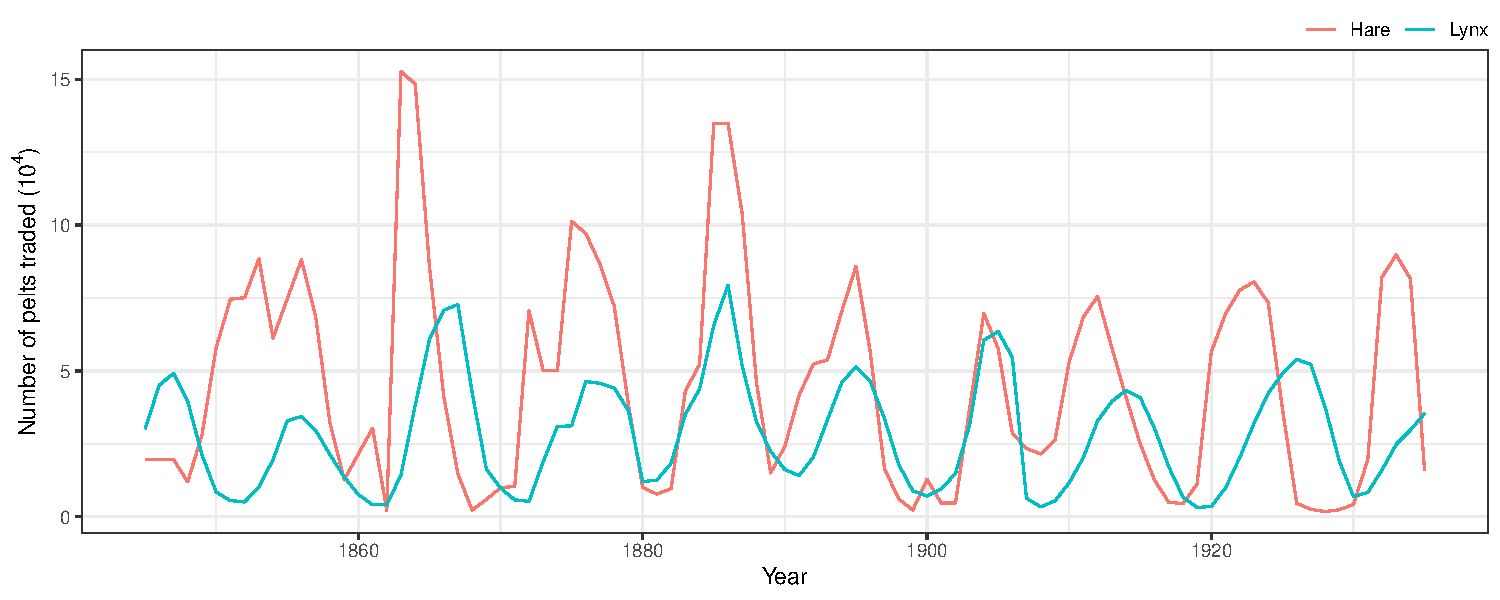
\includegraphics[width = \linewidth]{fig/simAR/lynxhare.pdf}
\caption{The Hudson Bay Company kept records of their trading (from all the company's operating regions) in Snowshoe Hare and Canadian Lynx furs from 1845 to 1935. The “pelt" dataset is available in \textsf{R} with the \texttt{tsibbledata} package \citep{ohara-wild2022}.}
\label{fig:lynxhare}
\end{figure}

We consider a $2$-level hierarchical structure with three time series in total: one upper series and two bottom series, with semi-annual data ($\mathcal{K} = \{2,1\}$). The cross-sectional aggregation matrix is
$
\Avet_{cs} = \begin{bmatrix}
1 & 1 \\
\end{bmatrix}
$.
This means that the upper series, $A$, is a combination of the two bottom series, $B$ and $C$, such that $A = B+C$.
The data for the bottom series $B$ and $C$ are generated by AR($2$) processes, where the AR parameters are estimated from the “Lynx" and “Hare" time series (see Figure \ref{fig:lynxhare}). The AR parameters for $B$ and $C$ are
$
\phi_B = \begin{bmatrix}
1.34 &
-0.74
\end{bmatrix}'$ and $\phi_C = \begin{bmatrix}
0.95 &
-0.42
\end{bmatrix}'
$,
respectively. The errors driving the AR processes are drawn from a multivariate normal distribution with standard deviations simulated from a uniform distribution between 0.5 and 2 and a fixed correlation of -0.8. The cross-sectional error covariance matrix is given by
$$
\Omegavet_{cs} = \begin{bmatrix}
0.9 & 0 \\
0 & 1.8
\end{bmatrix} \begin{bmatrix}
1 & \rho \\
\rho & 1
\end{bmatrix} \begin{bmatrix}
0.9 & 0 \\
0 & 1.8
\end{bmatrix} = \begin{bmatrix}
\sigma_B^2 & \sigma_{BC} \\
\sigma_{BC} & \sigma_C^2
\end{bmatrix}.
$$
The bottom series are then cross-temporally aggregated to obtain the series at any temporal aggregation.

For the forecast experiment, base forecasts using AR models will be used. The order of the AR models is not fixed at the true order, but rather is determined using the algorithm proposed by \cite{hyndman2008a} in the \textsf{R} package \texttt{forecast} \citep{Rforecast}. This allows for the possibility of mis-specification in the models. The training window length is 500 years, consisting of 1000 observations. The experiment will be replicated 500 times, with a forecast horizon of 1 year.

Since the models used for the data generating process (DPG) for the bottom series $B$ and $C$ at the most aggregated temporal level are two AR(2) models, we have calculated the true covariance matrix for one-step ahead forecasts at the annual level. Therefore, we have that $\Omegavet_{ct} = \Svet_{ct}\Omegavet_{hf-bts}\Svet_{ct}'$ where
$$
\Omegavet_{hf-bts} = \begin{bmatrix}
\sigma^2_B & & & \\
\phi_{B,1}\sigma_B^2 & \sigma_B^2\left(1+\phi_{B,1}^2\right) & & \\
\sigma_{BC} & \phi_{B,1}\sigma_{BC} & \sigma_C^2& \\
\phi_{C,1}\sigma_{BC} & \sigma_{BC}\left(1+\phi_{B,1}\phi_{C,1} \right)& \phi_{C,1}\sigma_C^2 & \sigma_C^2\left(1+\phi_{C,1}^2\right)\
\end{bmatrix}.
$$
The detailed calculations can be found in appendix \ref{app:ar2}.
In Figure \ref{fig:covcorMC} we have represented both the covariance matrix and the correlation matrix for fixed parameters.

\begin{figure}[t]
\centering
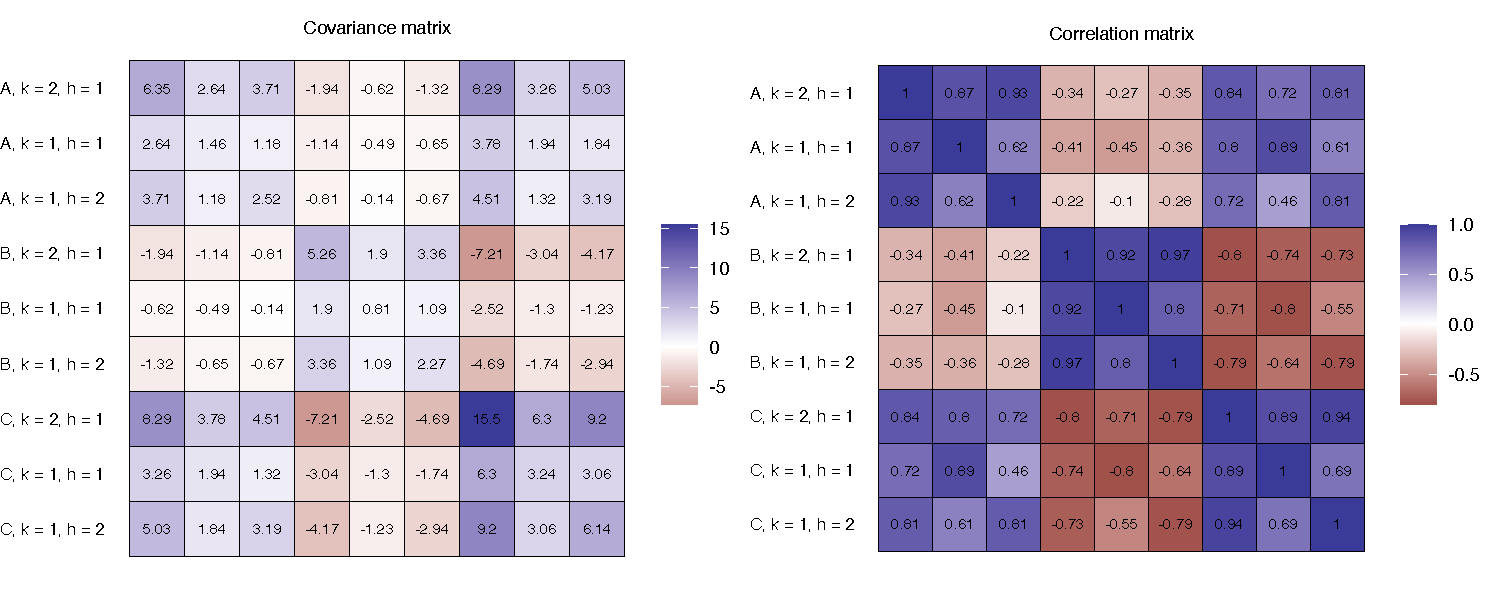
\includegraphics[width = \linewidth]{fig/simAR/covcor.pdf}
\caption{True cross-temporal covariance (left) and correlation (right) matrix of forecasts reconciled with $\sigma_B = 0.9$, $\sigma_C = 1.8$, $\phi_B =  \begin{bmatrix} 1.34 & -0.74 \end{bmatrix}'$, $\phi_C = \begin{bmatrix} 0.95 & -0.42 \end{bmatrix}'$ and $\rho = -0.8$.}
\label{fig:covcorMC}
\end{figure}

\subsection{Base and reconciled samples}\label{ssec:sim_br}
To construct cross-temporal samples of the base forecasts, we use the bootstrap and Gaussian approaches discussed in Sections \ref{ssec:boot} and \ref{ssec:prob_pf}, respectively. For the non-parametric approach, we use in-sample residuals, while for the parametric approach we use in-sample residuals and multi-step forecasting with the different covariance matrix structures analyzed in Section \ref{sec:shrtech}: $G$ for the global covariance matrix, $H$ for the High frequency covariance matrix, $B$ for the bottom time series covariance matrix and $HB$ for the high frequency bottom time series covariance matrix. We do not use overlapping residuals in our analysis because the large number of available observations made it unnecessary %and using overlapping residuals did not significantly affect the results of our analysis.

Regarding reconciliation, we have several options: cross-temporal bottom-up (\textit{ct bu}); cross-sectional reconciliation using the $shr$ approach (see Table \ref{tab:cov_app}) and then temporally aggregated (ct$(shr_{cs}, bu_{te})$, Section \ref{ssec:ctbu});  temporal reconciliation using the $wlsv$ approach (see Table \ref{tab:cov_app}) and then cross-sectionally aggregated (ct$(wlsv_{te}, bu_{cs})$, Section \ref{ssec:ctbu}); optimal cross-temporal reconciliation \citep{difonzo2023} with in-sample residuals (\textbf{oct}) using the $wlsv$, $bdshr$ approaches presented in Section \ref{ssec:oct}, and $shr$, $hshr$, $bshr$ and $hbshr$ approaches that use, respectively, the Global, High frequency, Bottom time series, High frequency Bottom time series shrinkage presented in Section \ref{sec:shrtech}. In addition, we propose the optimal cross-temporal reconciliation with multi-step residuals (\textbf{oct$_h$}) for $shr$, $hshr$, $bshr$ and $hbshr$ approaches. All this procedure are available in the \textsf{R} package \texttt{FoReco} \citep{girolimetto2022} that provides a set of functions and algorithms for point forecast reconciliation.

\subsection{A look at the covariance matrix}

Figure \ref{fig:ar2covcor} compares the estimated covariance and correlation matrices for base forecasts using different approaches. The first column represents the covariance matrix and the second column represents the correlation matrix. The first row uses a non-parametric bootstrap approach, while the second and third rows use a parametric Gaussian approach. The second row uses in-sample residuals and the third row uses multi-step residuals. The true covariance and correlation matrices are shown in Figure \ref{fig:covcorMC} for comparison. It is important to highlight that the correlations between the one-step and two-step ahead forecasts are almost always zero when the base forecasts are assumed to be normal and the covariance matrix is estimated using in-sample residuals. Similar results are observed when applying reconciliation.

To compare the true covariance matrix $\Omegavet_{ct}$ with the estimated covariance matrix $\Omegavet$, we use the Frobenius norm that is a metric that quantifies the difference between two matrices:
$$
\lVert \Dvet \rVert_F = \sqrt{\sum_{i = 1}^{n(k^\ast + m)}\sum_{j = 1}^{n(k^\ast + m)}|d_{i,j}|^2},
$$
where $\Dvet = \Omegavet - \Omegavet_{ct}$. The true covariance matrix, shown in Figure \ref{fig:covcorMC}, was compared to the estimated covariance matrix obtained using various reconciliation methods and techniques for base forecasts' samples. By comparing these two matrices using the Frobenius norm, we were able to determine which reconciliation method and simulation technique produce an accurate estimate of the covariance matrix. Other types of matrix norms were also used with similar results.

From Table \ref{tab:ar2norm}, it appears that the reconciled covariance matrices are always closer to the true matrix than the base forecast matrix when using the bootstrap technique. However, using in-sample residuals to estimate the covariance matrix in the Gaussian framework results in a matrix far from the “truth". On the other hand, when using multi-step residuals to estimate the covariance matrix, the results are more comparable to those obtained with the bootstrap technique, with the reconciliation improving the estimate of the covariance matrix. Overall, there are no difference in the findings when using either in-sample or multi-step residuals in cross-temporal reconciliation. In fact, using approaches like oct$(bdshr)$, we obtain outcomes that are consistent with the results obtained with covariance matrices like oct$_h(shr)$. It is worth noting that if we simulate the base forecasts using the $HB$ covariance matrix, then reconciliation does not modify it as we expected (see Section \ref{sec:shrtech}). In conclusion, our results suggest that using multi-step residuals or bootstrap techniques may help find an estimate of the covariance matrix close to its true counterpart, and that reconciliation can further improve this estimate.

\begin{figure}[p]
\centering
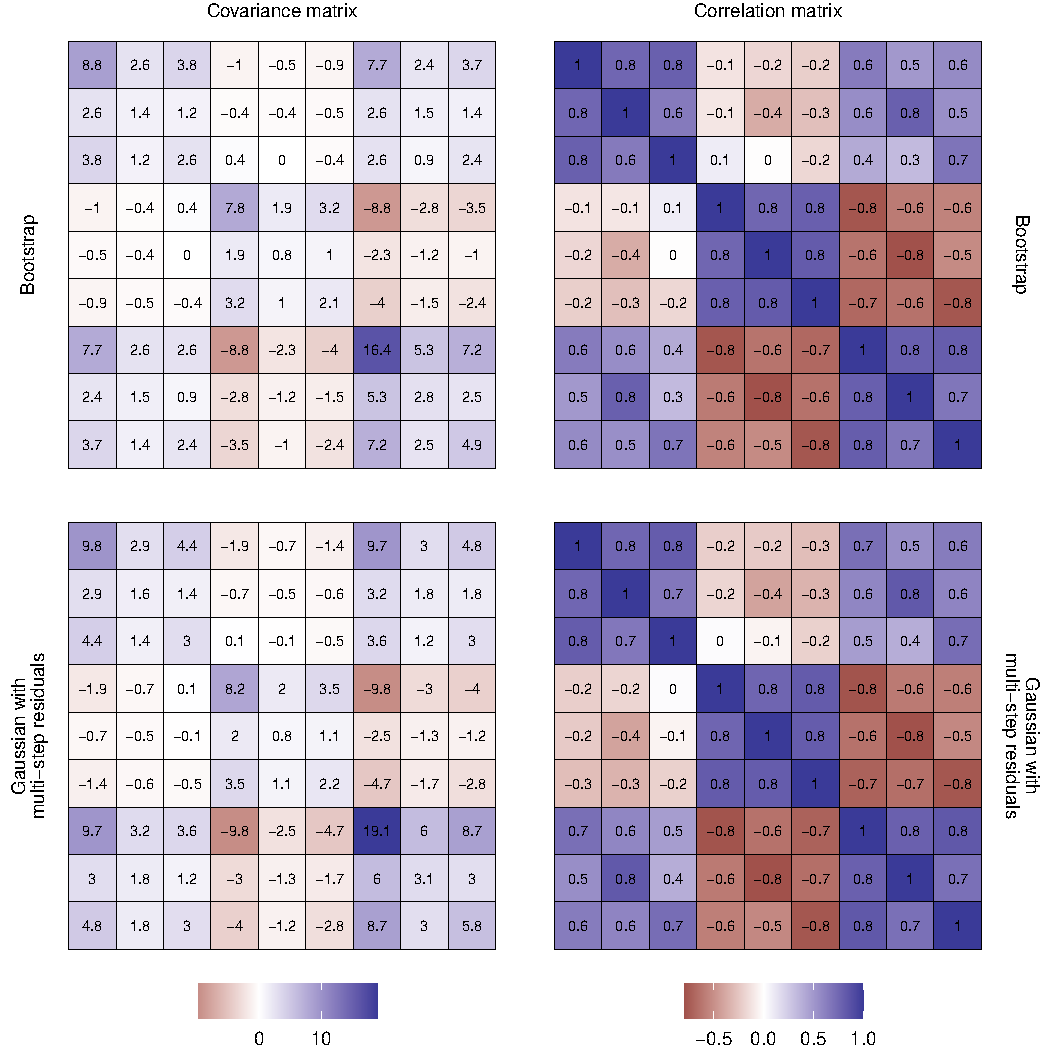
\includegraphics[width = 0.9\linewidth]{fig/simAR/base_cov.pdf}
\caption{Comparison of estimated covariance and correlation matrices for base forecasts using non-parametric bootstrap (first row) and parametric Gaussian (second and third rows) approaches. The second row uses in-sample residuals and the third row uses multi-step residuals. The true covariance and correlation matrices are shown in Figure \ref{fig:covcorMC}.}
\label{fig:ar2covcor}
\end{figure}

\begin{table}[t]
\centering
\fontsize{9}{11}\selectfont

\begin{tabular}[t]{l|>{}ccccc}
\toprule
\multicolumn{1}{c}{\textbf{}} & \multicolumn{5}{c}{\textbf{Generation of the base forecasts paths}} \\
\cmidrule(l{0pt}r{0pt}){2-6}
\multicolumn{1}{c}{\makecell[c]{\bfseries Reconciliation\\\bfseries approach}} & \multicolumn{1}{c}{ctjb} & \multicolumn{4}{c}{\makecell[c]{Gaussian approach\textsuperscript{*}}} \\
\multicolumn{1}{c}{} &  & G & B & H & HB\\
\midrule
base & \textcolor{black}{8.260} & \textcolor{black}{7.748} & \textcolor{black}{6.549} & \textcolor{black}{3.409} & \textcolor{black}{2.215}\\
ct$(bu)$ & \textcolor{black}{3.195} & \textcolor{black}{2.215} & \textcolor{black}{2.215} & \textcolor{black}{\textbf{2.215}} & \textcolor{black}{2.215}\\
ct$(shr_{cs}, bu_{te})$ & \textcolor{black}{3.202} & \textcolor{black}{2.224} & \textcolor{black}{2.215} & \textcolor{black}{2.224} & \textcolor{black}{2.215}\\
ct$(wlsv_{te}, bu_{cs})$ & \textcolor{black}{\textbf{3.183}} & \textcolor{black}{\textbf{2.188}} & \textcolor{black}{2.188} & \textcolor{black}{\textbf{2.215}} & \textcolor{black}{2.215}\\
oct$(wlsv)$ & \textcolor{black}{3.766} & \textcolor{black}{3.082} & \textcolor{black}{2.191} & \textcolor{black}{2.910} & \textcolor{black}{2.215}\\
oct$(bdshr)$ & \textcolor{black}{3.203} & \textcolor{black}{2.195} & \textcolor{blue}{\textbf{2.184}} & \textcolor{black}{2.224} & \textcolor{black}{\textbf{2.215}}\\
oct$_h(shr)$ & \textcolor{black}{3.251} & \textcolor{black}{2.260} & \textcolor{black}{2.202} & \textcolor{black}{2.226} & \textcolor{black}{2.215}\\
oct$_h(bshr)$ & \textcolor{black}{3.602} & \textcolor{black}{2.720} & \textcolor{black}{2.220} & \textcolor{black}{2.756} & \textcolor{black}{2.215}\\
oct$_h(hshr)$ & \textcolor{black}{4.869} & \textcolor{black}{4.138} & \textcolor{black}{4.167} & \textcolor{black}{2.225} & \textcolor{black}{2.215}\\
\bottomrule
\multicolumn{6}{l}{\rule{0pt}{1em}\rule{0pt}{1.75em}\makecell[l]{$^\ast$The Gaussian method employs a sample covariance\\ with multi-step residuals.}}\\
\end{tabular}

\caption{Frobenius norm between the true (in Figure \ref{fig:covcorMC}) and the estimated covariance matrix for different reconciliation approaches and different techniques for simulating the base forecasts. In bold, it is reported the lowest value for each column, in blue the minimum.  The notation used to refer to the reconciliation and base forecast samples is explained in more detail in Section \ref{ssec:sim_br}.}
\label{tab:ar2norm}
\end{table}

\subsection{Accuracy scores}\label{ssec:acc_scores}

The accuracy of the probabilistic forecasts is evaluated using the Continuous Ranked Probability Score (CRPS, \citealp{gneiting2014}), given by
\begin{equation}\label{eq:crps}
	\operatorname{CRPS}(\hat{P}_i, z_i)=\frac{1}{L} \sum_{l=1}^{L}\left|x_{i,l}-z_i\right|-\frac{1}{2 L^{2}} \sum_{l=1}^{L} \sum_{j=1}^{L}\left|x_{i,l}-x_{i,j}\right|, \quad i = 1,\dots,n,
\end{equation}
where $\hat{P}_i(\omega)=\frac{1}{L} \sum_{l=1}^{L} \mathbf{1}\left(x_{i,l} \leq \omega\right)$, $\xvet_{1}, \xvet_{2}, \ldots, \xvet_{L}\in \mathbb{R}^{n}$ is a collection of $L$ random draws taken from the predictive distribution and $\zvet \in \mathbb{R}^{n}$ is the observation vector. This scoring rule is implemented in the \textsf{R} package \texttt{scoringRules} \citep{jordan2019}. CRPS is an index that considers the single series and provides us a marginal evaluation of the approaches.
In addition, we employ the Energy Score (ES, \citealp{gneiting2014}), that is the CRPS extension to the multivariate case, to evaluate the forecasting accuracy for the whole system \citep{wickramasuriya2021b, panagiotelis2023} ,
\begin{equation}\label{eq:es}
\operatorname{ES}(\hat{P}, \zvet)=\frac{1}{L} \sum_{l=1}^{L}\left\|\xvet_{l}-\zvet\right\|_{2}-\frac{1}{2(L-1)} \sum_{i=1}^{L-1}\left\|\xvet_{l}-\xvet_{l+1}\right\|_{2}
\end{equation}

In Tables 5 and 6 are reported the results using these two indices. In
particular, we consider the geometric mean of the skill scores of the
CRPS indices \citep{fleming1986}, and the standard skill score
for index ES:
\begin{equation}\label{eq:skill}
	\operatorname{ScoreCRPS}_{j,s}^{[k]} = \left(\prod_{i = 1}^n \frac{CRPS^{[k]}_{i, j, s}}{CRPS^{[k]}_{i, 0, 0}}\right)^{\frac{1}{n}} \qquad \mathrm{and} \qquad \operatorname{ScoreES}_{j,s}^{[k]} = \frac{ES^{[k]}_{j, s}}{ES^{[k]}_{0, 0}}
\end{equation}
where $j$ indicates the reconciliation approach used (first two columns of the tables), $s$ indicates the approach used to simulate the base forecasts (the remaining columns). As a reference approach ($s=0$ and $j=0$), we consider the base forecasts using the Gaussian approach (sample covariance matrix) estimating the covariance matrix with all the residuals ($G$). Low values of these indicators mean a better quality of the forecasts. If we consider all the temporal aggregation orders (i.e. $\forall k \in \{2,1\}$), we use the geometric averages
\begin{equation}\label{eq:skillCRPS_all}
	\operatorname{ScoreCRPS}_{j,s} = \left(\prod_{\substack{i = 1, \dots, n \\ k \in \{1,2\}}}\frac{CRPS^{[k]}_{i, j, s}}{CRPS^{[k]}_{i, 0, 0}}\right)^{\frac{1}{n(k^\ast+m)}},
\end{equation}
and
\begin{equation}\label{eq:skillES_all}
	\operatorname{ScoreES}_{j,s}= \left(\prod_{k \in \{1,2\}}\frac{ES^{[k]}_{j, s}}{ES^{[k]}_{0, 0}}\right)^{\frac{1}{(k^\ast+m)}}.
\end{equation}
A limitation of this simulation experiment is that we are using a high number of residuals, which may result in a potential loss of benefit when using forms of covariance matrix parameterization such as $HB$, $H$, or $B$ (see Section \ref{sec:shrtech}). Additionally, shrinkage techniques often yield very similar, results when we use the corresponding matrix with $\lambda = 0$ (full covariance matrix). It is important to consider these limitations when interpreting the results.

\begin{table}[p]
\centering
\begingroup
\spacingset{1}
\fontsize{9}{11}\selectfont

\begin{tabular}[t]{c|>{}cccc>{}c|ccccc}
\toprule
\multicolumn{1}{c}{\textbf{}} & \multicolumn{10}{c}{\textbf{Base forecasts' sample approach}} \\
\cmidrule(l{0pt}r{0pt}){2-11}
\multicolumn{1}{c}{\makecell[c]{\bfseries Reconciliation\\\bfseries approach}} & \multicolumn{1}{c}{ctjb} & \multicolumn{4}{c}{\makecell[c]{Gaussian approach\textsuperscript{*}}} & \multicolumn{1}{c}{ctjb} & \multicolumn{4}{c}{\makecell[c]{Gaussian approach\textsuperscript{*}}} \\
\multicolumn{1}{c}{} &  & G & B & H & \multicolumn{1}{c}{HB} &  & G & B & H & HB\\
\midrule
\addlinespace[0.3em]
\multicolumn{1}{c}{} & \multicolumn{5}{c}{\textbf{$\forall k \in \{12,6,4,3,2,1\}$}} & \multicolumn{5}{c}{\textbf{$k = 1$}}\\
base & \textcolor{black}{1.000} & \textcolor{black}{0.971} & \textcolor{black}{0.971} & \textcolor{black}{0.973} & \textcolor{black}{0.973} & \textcolor{black}{1.000} & \textcolor{black}{0.972} & \textcolor{black}{0.972} & \textcolor{black}{0.972} & \textcolor{black}{0.972}\\
ct$(bu)$ & \textcolor{red}{1.321} & \textcolor{red}{1.011} & \textcolor{red}{1.011} & \textcolor{red}{1.011} & \textcolor{red}{1.011} & \textcolor{red}{1.077} & \textcolor{black}{0.983} & \textcolor{black}{0.982} & \textcolor{black}{0.982} & \textcolor{black}{0.982}\\
ct$(shr_{cs}, bu_{te})$ & \textcolor{red}{1.057} & \textcolor{black}{0.974} & \textcolor{black}{0.969} & \textcolor{black}{0.974} & \textcolor{black}{0.969} & \textcolor{black}{0.976} & \textcolor{black}{0.963} & \textcolor{black}{0.962} & \textcolor{black}{0.963} & \textcolor{black}{0.962}\\
ct$(wls_{cs}, bu_{te})$ & \textcolor{red}{1.082} & \textcolor{black}{0.977} & \textcolor{black}{0.976} & \textcolor{black}{0.977} & \textcolor{black}{0.976} & \textcolor{black}{0.986} & \textcolor{black}{0.965} & \textcolor{black}{0.965} & \textcolor{black}{0.965} & \textcolor{black}{0.965}\\
oct$(wlsv)$ & \textcolor{black}{0.987} & \textcolor{black}{0.959} & \textcolor{black}{0.959} & \textcolor{black}{0.958} & \textcolor{black}{0.957} & \textcolor{black}{0.952} & \textcolor{black}{0.957} & \textcolor{black}{0.957} & \textcolor{black}{0.957} & \textcolor{black}{0.957}\\
oct$(bdshr)$ & \textcolor{black}{\textbf{0.975}} & \textcolor{black}{\textbf{0.956}} & \textcolor{black}{\textbf{0.953}} & \textcolor{black}{\textbf{0.952}} & \textcolor{blue}{\textbf{0.951}} & \textcolor{blue}{\textbf{0.949}} & \textcolor{black}{\textbf{0.955}} & \textcolor{black}{\textbf{0.953}} & \textcolor{black}{\textbf{0.954}} & \textcolor{black}{\textbf{0.954}}\\
\addlinespace[0.3em]
\multicolumn{1}{c}{} & \multicolumn{5}{c}{\textbf{$k = 2$}} & \multicolumn{5}{c}{\textbf{$k = 3$}}\\
base & \textcolor{black}{1.000} & \textcolor{black}{0.970} & \textcolor{black}{0.969} & \textcolor{black}{0.970} & \textcolor{black}{0.971} & \textcolor{black}{1.000} & \textcolor{black}{0.971} & \textcolor{black}{0.971} & \textcolor{black}{0.972} & \textcolor{black}{0.973}\\
ct$(bu)$ & \textcolor{red}{1.189} & \textcolor{black}{0.999} & \textcolor{black}{0.999} & \textcolor{black}{0.999} & \textcolor{black}{0.999} & \textcolor{red}{1.273} & \textcolor{red}{1.010} & \textcolor{red}{1.010} & \textcolor{red}{1.010} & \textcolor{red}{1.010}\\
ct$(shr_{cs}, bu_{te})$ & \textcolor{red}{1.015} & \textcolor{black}{0.972} & \textcolor{black}{0.970} & \textcolor{black}{0.972} & \textcolor{black}{0.970} & \textcolor{red}{1.041} & \textcolor{black}{0.977} & \textcolor{black}{0.974} & \textcolor{black}{0.977} & \textcolor{black}{0.974}\\
ct$(wls_{cs}, bu_{te})$ & \textcolor{red}{1.031} & \textcolor{black}{0.975} & \textcolor{black}{0.974} & \textcolor{black}{0.975} & \textcolor{black}{0.974} & \textcolor{red}{1.062} & \textcolor{black}{0.980} & \textcolor{black}{0.979} & \textcolor{black}{0.980} & \textcolor{black}{0.979}\\
oct$(wlsv)$ & \textcolor{black}{0.972} & \textcolor{black}{0.961} & \textcolor{black}{0.960} & \textcolor{black}{0.960} & \textcolor{black}{0.960} & \textcolor{black}{0.983} & \textcolor{black}{0.963} & \textcolor{black}{0.962} & \textcolor{black}{0.962} & \textcolor{black}{0.962}\\
oct$(bdshr)$ & \textcolor{black}{\textbf{0.964}} & \textcolor{black}{\textbf{0.958}} & \textcolor{black}{\textbf{0.957}} & \textcolor{black}{\textbf{0.956}} & \textcolor{blue}{\textbf{0.956}} & \textcolor{black}{\textbf{0.972}} & \textcolor{black}{\textbf{0.960}} & \textcolor{black}{\textbf{0.958}} & \textcolor{black}{\textbf{0.957}} & \textcolor{blue}{\textbf{0.957}}\\
\addlinespace[0.3em]
\multicolumn{1}{c}{} & \multicolumn{5}{c}{\textbf{$k = 4$}} & \multicolumn{5}{c}{\textbf{$k = 6$}}\\
base & \textcolor{black}{1.000} & \textcolor{black}{0.973} & \textcolor{black}{0.973} & \textcolor{black}{0.974} & \textcolor{black}{0.975} & \textcolor{black}{1.000} & \textcolor{black}{0.976} & \textcolor{black}{0.976} & \textcolor{black}{0.978} & \textcolor{black}{0.978}\\
ct$(bu)$ & \textcolor{red}{1.340} & \textcolor{red}{1.016} & \textcolor{red}{1.015} & \textcolor{red}{1.015} & \textcolor{red}{1.015} & \textcolor{red}{1.450} & \textcolor{red}{1.023} & \textcolor{red}{1.023} & \textcolor{red}{1.023} & \textcolor{red}{1.023}\\
ct$(shr_{cs}, bu_{te})$ & \textcolor{red}{1.061} & \textcolor{black}{0.978} & \textcolor{black}{0.973} & \textcolor{black}{0.978} & \textcolor{black}{0.973} & \textcolor{red}{1.094} & \textcolor{black}{0.978} & \textcolor{black}{0.972} & \textcolor{black}{0.978} & \textcolor{black}{0.972}\\
ct$(wls_{cs}, bu_{te})$ & \textcolor{red}{1.087} & \textcolor{black}{0.982} & \textcolor{black}{0.980} & \textcolor{black}{0.982} & \textcolor{black}{0.980} & \textcolor{red}{1.127} & \textcolor{black}{0.982} & \textcolor{black}{0.981} & \textcolor{black}{0.982} & \textcolor{black}{0.981}\\
oct$(wlsv)$ & \textcolor{black}{0.990} & \textcolor{black}{0.962} & \textcolor{black}{0.961} & \textcolor{black}{0.961} & \textcolor{black}{0.960} & \textcolor{red}{1.001} & \textcolor{black}{0.960} & \textcolor{black}{0.959} & \textcolor{black}{0.958} & \textcolor{black}{0.957}\\
oct$(bdshr)$ & \textcolor{black}{\textbf{0.977}} & \textcolor{black}{\textbf{0.959}} & \textcolor{black}{\textbf{0.956}} & \textcolor{black}{\textbf{0.955}} & \textcolor{blue}{\textbf{0.954}} & \textcolor{black}{\textbf{0.985}} & \textcolor{black}{\textbf{0.956}} & \textcolor{black}{\textbf{0.953}} & \textcolor{black}{\textbf{0.950}} & \textcolor{blue}{\textbf{0.948}}\\
\addlinespace[0.3em]
\multicolumn{1}{c}{} & \multicolumn{5}{c}{\textbf{$k = 12$}} & \multicolumn{5}{c}{}\\
base & \textcolor{black}{\textbf{1.000}} & \textcolor{black}{0.968} & \textcolor{black}{0.967} & \textcolor{black}{0.969} & \textcolor{black}{0.969} &  &  &  &  & \\
ct$(bu)$ & \textcolor{red}{1.675} & \textcolor{red}{1.038} & \textcolor{red}{1.037} & \textcolor{red}{1.037} & \textcolor{red}{1.038} &  &  &  &  & \\
ct$(shr_{cs}, bu_{te})$ & \textcolor{red}{1.163} & \textcolor{black}{0.977} & \textcolor{black}{0.965} & \textcolor{black}{0.977} & \textcolor{black}{0.965} &  &  &  &  & \\
ct$(wls_{cs}, bu_{te})$ & \textcolor{red}{1.212} & \textcolor{black}{0.980} & \textcolor{black}{0.976} & \textcolor{black}{0.980} & \textcolor{black}{0.976} &  &  &  &  & \\
oct$(wlsv)$ & \textcolor{red}{1.025} & \textcolor{black}{0.954} & \textcolor{black}{0.953} & \textcolor{black}{0.949} & \textcolor{black}{0.947} &  &  &  &  & \\
oct$(bdshr)$ & \textcolor{red}{1.002} & \textcolor{black}{\textbf{0.950}} & \textcolor{black}{\textbf{0.944}} & \textcolor{black}{\textbf{0.939}} & \textcolor{blue}{\textbf{0.935}} &  &  &  &  & \\
\bottomrule
\multicolumn{11}{l}{\rule{0pt}{1em}\rule{0pt}{2em}\textsuperscript{*}\makecell[l]{The Gaussian method employs a sample covariance matrix and includes four techniques (G, B, H, HB)\\ with multi-step residuals.}}\\
\end{tabular}

\endgroup
\caption{CRPS skill score defined in (\ref{eq:skill}) and (\ref{eq:skillCRPS_all}). The smaller this value, the more accurate the forecast. Approaches that performed worse than the benchmark model (base, $G$) are highlighted in red, the best for each column is marked in bold, and the overall lowest value is highlighted in blue. The notation used to refer to the reconciliation and base forecast samples is explained in Section \ref{ssec:sim_br}.}
\label{tab:ar2crps}
\end{table}

\begin{table}[p]
\centering
\begingroup
\spacingset{1}
\fontsize{9}{11}\selectfont

\begin{tabular}[t]{c|>{}cccc>{}c|ccccc}
\toprule
\multicolumn{1}{c}{\textbf{}} & \multicolumn{10}{c}{\textbf{Base forecasts' sample approach}} \\
\cmidrule(l{0pt}r{0pt}){2-11}
\multicolumn{1}{c}{\makecell[c]{\bfseries Reconciliation\\\bfseries approach}} & \multicolumn{1}{c}{ctjb} & \multicolumn{4}{c}{\makecell[c]{Gaussian approach\textsuperscript{*}}} & \multicolumn{1}{c}{ctjb} & \multicolumn{4}{c}{\makecell[c]{Gaussian approach\textsuperscript{*}}} \\
\multicolumn{1}{c}{} &  & G$_{h}$ & H$_{h}$ & G$_{oh}$ & \multicolumn{1}{c}{H$_{oh}$} &  & G$_{h}$ & H$_{h}$ & G$_{oh}$ & \multicolumn{1}{c}{H$_{oh}$}\\
\midrule
\addlinespace[0.3em]
\multicolumn{1}{c}{} & \multicolumn{5}{c}{\textbf{$\forall k \in \{4,2,1\}$}} & \multicolumn{5}{c}{\textbf{$k = 1$}}\\
base & \textcolor{black}{1.000} & \textcolor{black}{0.970} & \textcolor{black}{0.988} & \textcolor{black}{0.960} & \textcolor{black}{0.970} & \textcolor{black}{1.000} & \textcolor{black}{0.977} & \textcolor{black}{0.977} & \textcolor{black}{0.965} & \textcolor{black}{0.965}\\
ct$(shr_{cs}, bu_{te})$ & \textcolor{black}{0.897} & \textcolor{black}{0.944} & \textcolor{black}{0.944} & \textcolor{black}{0.973} & \textcolor{black}{0.973} & \textcolor{black}{0.964} & \textcolor{red}{1.001} & \textcolor{red}{1.001} & \textcolor{red}{1.033} & \textcolor{red}{1.033}\\
ct$(wls_{cs}, bu_{te})$ & \textcolor{black}{\textbf{0.886}} & \textcolor{black}{0.880} & \textcolor{black}{\textbf{0.880}} & \textcolor{blue}{\textbf{0.860}} & \textcolor{black}{\textbf{0.860}} & \textcolor{black}{\textbf{0.954}} & \textcolor{black}{\textbf{0.944}} & \textcolor{black}{\textbf{0.945}} & \textcolor{blue}{\textbf{0.928}} & \textcolor{black}{\textbf{0.928}}\\
oct$_o(wlsv)$ & \textcolor{black}{0.891} & \textcolor{black}{\textbf{0.879}} & \textcolor{black}{0.881} & \textcolor{black}{0.864} & \textcolor{black}{0.864} & \textcolor{black}{0.958} & \textcolor{black}{0.945} & \textcolor{black}{0.945} & \textcolor{black}{0.931} & \textcolor{black}{0.931}\\
oct$_o(bdshr)$ & \textcolor{black}{0.940} & \textcolor{black}{0.928} & \textcolor{black}{0.910} & \textcolor{black}{0.918} & \textcolor{black}{0.895} & \textcolor{red}{1.004} & \textcolor{black}{0.986} & \textcolor{black}{0.971} & \textcolor{black}{0.980} & \textcolor{black}{0.961}\\
oct$_{oh}(shr)$ & \textcolor{red}{1.059} & \textcolor{red}{1.015} & \textcolor{black}{0.956} & \textcolor{red}{1.053} & \textcolor{black}{0.945} & \textcolor{red}{1.130} & \textcolor{red}{1.063} & \textcolor{red}{1.019} & \textcolor{red}{1.121} & \textcolor{red}{1.016}\\
oct$_{oh}(hshr)$ & \textcolor{black}{0.986} & \textcolor{black}{0.968} & \textcolor{black}{0.999} & \textcolor{black}{0.959} & \textcolor{black}{0.992} & \textcolor{red}{1.053} & \textcolor{red}{1.034} & \textcolor{red}{1.049} & \textcolor{red}{1.024} & \textcolor{red}{1.055}\\
\addlinespace[0.3em]
\multicolumn{1}{c}{} & \multicolumn{5}{c}{\textbf{$k = 2$}} & \multicolumn{5}{c}{\textbf{$k = 4$}}\\
base & \textcolor{black}{1.000} & \textcolor{black}{0.972} & \textcolor{black}{0.985} & \textcolor{black}{0.959} & \textcolor{black}{0.969} & \textcolor{black}{1.000} & \textcolor{black}{0.959} & \textcolor{red}{1.000} & \textcolor{black}{0.957} & \textcolor{black}{0.976}\\
ct$(shr_{cs}, bu_{te})$ & \textcolor{black}{0.915} & \textcolor{black}{0.961} & \textcolor{black}{0.960} & \textcolor{black}{0.991} & \textcolor{black}{0.991} & \textcolor{black}{0.818} & \textcolor{black}{0.874} & \textcolor{black}{0.874} & \textcolor{black}{0.899} & \textcolor{black}{0.900}\\
ct$(wls_{cs}, bu_{te})$ & \textcolor{black}{\textbf{0.904}} & \textcolor{black}{0.896} & \textcolor{black}{\textbf{0.896}} & \textcolor{blue}{\textbf{0.877}} & \textcolor{black}{\textbf{0.877}} & \textcolor{black}{\textbf{0.807}} & \textcolor{black}{0.805} & \textcolor{black}{\textbf{0.805}} & \textcolor{blue}{\textbf{0.782}} & \textcolor{black}{\textbf{0.783}}\\
oct$_o(wlsv)$ & \textcolor{black}{0.908} & \textcolor{black}{\textbf{0.895}} & \textcolor{black}{0.898} & \textcolor{black}{0.881} & \textcolor{black}{0.882} & \textcolor{black}{0.812} & \textcolor{black}{\textbf{0.802}} & \textcolor{black}{0.806} & \textcolor{black}{0.786} & \textcolor{black}{0.786}\\
oct$_o(bdshr)$ & \textcolor{black}{0.960} & \textcolor{black}{0.947} & \textcolor{black}{0.929} & \textcolor{black}{0.938} & \textcolor{black}{0.915} & \textcolor{black}{0.860} & \textcolor{black}{0.856} & \textcolor{black}{0.836} & \textcolor{black}{0.841} & \textcolor{black}{0.816}\\
oct$_{oh}(shr)$ & \textcolor{red}{1.082} & \textcolor{red}{1.029} & \textcolor{black}{0.973} & \textcolor{red}{1.076} & \textcolor{black}{0.963} & \textcolor{black}{0.971} & \textcolor{black}{0.954} & \textcolor{black}{0.882} & \textcolor{black}{0.967} & \textcolor{black}{0.861}\\
oct$_{oh}(hshr)$ & \textcolor{red}{1.007} & \textcolor{black}{0.988} & \textcolor{red}{1.017} & \textcolor{black}{0.979} & \textcolor{red}{1.014} & \textcolor{black}{0.904} & \textcolor{black}{0.888} & \textcolor{black}{0.934} & \textcolor{black}{0.881} & \textcolor{black}{0.913}\\
\bottomrule
\multicolumn{11}{l}{\rule{0pt}{1em}\rule{0pt}{1.75em}\makecell[l]{$^\ast$The Gaussian method employs a sample covariance matrix:\\G$_{h}$ and H$_{h}$ use multi-step residuals and G$_{oh}$ and H$_{oh}$ use overlapping and multi-step residuals.}}\\
\end{tabular}

\endgroup
\caption{ES skill score defined in equation (\ref{eq:skill}) and (\ref{eq:skillES_all}). The smaller this value, the more accurate the forecast. Approaches that performed worse than the benchmark model (base, $G$) are highlighted in red, the best for each column is marked in bold, and the overall lowest value is highlighted in blue. The notation used to refer to the reconciliation and base forecast samples is explained in Section \ref{ssec:sim_br}.}
\label{tab:ar2es}
\end{table}

The \textit{ct bu} (cross-temporal bottom-up) approach is a reconciliation method that starts by base forecasts at the lowest level of aggregation (bottom base forecasts for $k = 1$), and then aggregates the reconciled forecasts up to the highest level of aggregation. The good performance of the \textit{ct bu} approach can be explained by a good quality of base forecasts at the bottom level for $k=1$ and therefore it is difficult for the other approaches to correctly adjust them using the somewhat less good forecasts of the higher temporal and cross-sectional levels. This also explains the good performance of ct$(shr_{cs}, bu_{te})$, which by definition only takes into account the information provided by the most temporally disaggregated base forecasts.

The index based on CRPS is lower when using multi-step residuals to simulate the base forecasts, compared to the cases where in-sample residuals are used. Introducing the correlation between different forecasting horizons means that the residuals at different steps are not assumed to be independent of each other, but are instead assumed to be correlated (see the previous section). This can lead to an improvement in the base forecasts, as the model is able to capture the dependence between the residuals at different steps. This improvement can also affect the reconciliations, as the quality of the base forecasts is an important factor in the reconciliation process. This indicates that the base forecasts are of better quality when simulated using multi-step residuals. However, this improvement does not extend to the use of multi-step residuals in the reconciliation process. In fact, there does not seem to be any advantage in using multi-step residuals to calculate the covariance matrix in the reconciliation process, as the value of the index is not significantly different when using in-sample or multi-step residuals in this case.

In conclusion, we explored the use of simulation and reconciliation techniques to improve the accuracy of forecasts. We found that simulating base forecasts from multi-step residuals resulted in an estimate of the covariance matrix that was closest to the true one. Additionally, we observed that reconciliation could be used to further improve the accuracy of these estimates. However, we also discovered that reconciliation did not offer much advantage when starting from a “good" base sample (in terms of CRPS and ES), whether using in-sample or multi-step residuals. On the other hand, using multi-step residuals corrected the lack of correlation when simulating from in-sample residuals. We obtained good base forecasts for $k=1$, which favored good performance for bottom-up techniques. Optimal cross-temporal reconciliation techniques, such as $wlsv$ and $bdshr$, which assume either zero temporal/cross-sectional correlations or a cross-sectional correlation structure equal for each level of temporal aggregation, respectively, were able to achieve good results in terms of both CRPS and ES.

\section{Australian GDP dataset}\label{sec:ausgdp}

The Australian Quarterly National Accounts dataset (AusGDP) has been widely used in the literature for cross-sectional and cross-temporal reconciliation. In particular, \cite{athanasopoulos2020} proposed using state-of-the-art forecast reconciliation methods to improve the accuracy of macroeconomic forecasts and facilitate aligned decision-making. In their empirical analysis, they applied cross-sectional forecast reconciliation to 95 Australian Quarterly National Accounts time series that represent the Gross Domestic Product (GDP) calculated using both the income and expenditure approaches. These two approaches correspond to two distinct hierarchical structures, with GDP at the top and 15 lower-level aggregates in the income approach, and GDP as the top-level aggregate in a hierarchy of 79 time series in the expenditure approach (for more information, see \citealp{athanasopoulos2020}, pp. 702-705 and figures 21.4-21.7).
\cite{bisaglia2020} showed how to obtain a one-number forecast where the GDP reconciled forecasts are coherent for both the expenditure and income sides.
 \cite{giro2022, difonzo2022c} extended the one number forecasts idea to the fully reconciled probabilistic forecasts, and \cite{difonzo2023} to point reconciliation in a cross-temporal framework

Building on the results of this analysis, probabilistic cross-temporal forecast reconciliation is now applied within the same forecasting experiment designed by \cite{difonzo2023}, which is the cross-temporal extension of the cross-sectional forecasting experiment in \cite{athanasopoulos2020}.
Univariate ARIMA models were used to obtain quarterly base forecasts for the $n = 95$ separate time series (over the period 1984:Q4 -- 2018:Q1), using the \texttt{auto.arima} function from the \textsf{R}-package \texttt{forecast} \citep{Rforecast}. The forecasting experiment used a recursive training sample with an expanding window: the first training sample spanned from 1984:Q4 to 1994:Q3, and the last ended on 2017:Q1, for a total of 91 forecast origins. In addition, one-step-ahead and two-step-ahead forecasts were also computed for time series obtained by aggregating two successive quarters and one-step-ahead forecasts were computed for time series obtained by aggregating four successive quarters.

%Univariate models have a number of advantages that make them useful in a variety of situations. One key advantage is their simplicity and ease of interpretation. Univariate models only consider a single variable, making them easier to understand and interpret compared to multivariate models which consider multiple variables. Another advantage of univariate models is their computational efficiency. Because they only consider a single variable, univariate models require fewer calculations and can be run more quickly compared to multivariate models. This can be especially useful when working with large datasets or when the analysis needs to be done in a short amount of time. While they may not be the best choice for every situation, univariate models have a number of advantages that make them a useful tool for analyzing data in a variety of situations.

\subsection{Base and reconciled samples}\label{ssec:aus_br}

To construct the base forecasts samples in the Gaussian case, we used the \textit{Global} (G) and \textit{High frequency} (H) sample covariance matrices presented in Section \ref{sec:shrtech} (the results with shrinkage version are available in the online appendix), since it is not possible to identify a unique representation \citep{giro2022} for the other two structures \textit{High frequency Bottom time series} (HB) and \textit{Bottom time series} (B). In addition, we will use multi-step residuals with and without overlapping to calculate these quantities, as the number of residuals available is very small compared to the cross-temporal dimensions presented in Table \ref{tab:num_param_data}. In the nonparametric case, we use the cross-temporal joint bootstrap presented in Section \ref{ssec:boot}.
Finally, to reconcile the resulting (1000) base forecasts samples, we have used the following techniques using the \textsf{R}-package \texttt{FoReco} \citep{girolimetto2022}:
\begin{itemize}[nosep, leftmargin = 2.5cm]
	\item[\textbf{ct}$(\;\cdot\;, bu_{te})$] partly bottom-up (Section \ref{ssec:ctbu}) starting from cross-sectional reconciled forecasts using the $shr$ and $wls$ approaches (Table \ref{tab:cov_app});
	\item[\textbf{oct}$_o(\;\cdot\;)$] optimal cross-temporal reconciliation with overlapping residuals for the $wlsv$ (Section \ref{ssec:oct}), $bdshr$ (Section \ref{ssec:oct}), $shr$ (\textit{Global shrinkage} in Section \ref{sec:shrtech}), and $hshr$ (\textit{High frequency shrinkage} in Section \ref{sec:shrtech}) approaches;
	\item[\textbf{oct}$_{oh}(\;\cdot\;)$] optimal cross-temporal reconciliation with overlapping and multi-step residuals for the $shr$ (\textit{Global shrinkage} in Section \ref{sec:shrtech}) and $hshr$ (\textit{High frequency shrinkage} in Section \ref{sec:shrtech}) approaches.
\end{itemize}
In the online appendix, we also report the results using in-sample residuals in the reconciliation.

To accurately evaluate the quality of our forecasts, we used the Continuous Ranked Probability Score (CRPS) and the Extreme Score (ES). These measures are detailed in formulas (\ref{eq:crps}) and (\ref{eq:es}), respectively, along with their corresponding skill scores (\ref{eq:skill}), (\ref{eq:skillCRPS_all}), and (\ref{eq:skillES_all}).
In order to provide a comprehensive understanding of our evaluation results, we will present and analyze these accuracy indices at multiple temporal levels. This will allow us to examine the performance of our forecasting techniques at different durations, giving us a more complete picture of their effectiveness.
Additionally, we utilized the non-parametric Friedman test and the post hoc “Multiple Comparison with the Best" (MCB) Nemenyi test \citep{koning2005, kourentzes2019, makridakis2022} to determine if the forecasting performances of the different techniques are significantly different from one another.

\subsection{Results}
\begin{table}[p]
\centering
\begingroup
\spacingset{1}
\fontsize{9}{11}\selectfont

\begin{tabular}[t]{c|>{}cccc>{}c|ccccc}
\toprule
\multicolumn{1}{c}{\textbf{}} & \multicolumn{10}{c}{\textbf{Base forecasts' sample approach}} \\
\cmidrule(l{0pt}r{0pt}){2-11}
\multicolumn{1}{c}{\makecell[c]{\bfseries Reconciliation\\\bfseries approach}} & \multicolumn{1}{c}{ctjb} & \multicolumn{4}{c}{\makecell[c]{Gaussian approach\textsuperscript{*}}} & \multicolumn{1}{c}{ctjb} & \multicolumn{4}{c}{\makecell[c]{Gaussian approach\textsuperscript{*}}} \\
\multicolumn{1}{c}{} &  & G & B & H & \multicolumn{1}{c}{HB} &  & G & B & H & HB\\
\midrule
\addlinespace[0.3em]
\multicolumn{1}{c}{} & \multicolumn{5}{c}{\textbf{$\forall k \in \{12,6,4,3,2,1\}$}} & \multicolumn{5}{c}{\textbf{$k = 1$}}\\
base & \textcolor{black}{1.000} & \textcolor{black}{0.971} & \textcolor{black}{0.971} & \textcolor{black}{0.973} & \textcolor{black}{0.973} & \textcolor{black}{1.000} & \textcolor{black}{0.972} & \textcolor{black}{0.972} & \textcolor{black}{0.972} & \textcolor{black}{0.972}\\
ct$(bu)$ & \textcolor{red}{1.321} & \textcolor{red}{1.011} & \textcolor{red}{1.011} & \textcolor{red}{1.011} & \textcolor{red}{1.011} & \textcolor{red}{1.077} & \textcolor{black}{0.983} & \textcolor{black}{0.982} & \textcolor{black}{0.982} & \textcolor{black}{0.982}\\
ct$(shr_{cs}, bu_{te})$ & \textcolor{red}{1.057} & \textcolor{black}{0.974} & \textcolor{black}{0.969} & \textcolor{black}{0.974} & \textcolor{black}{0.969} & \textcolor{black}{0.976} & \textcolor{black}{0.963} & \textcolor{black}{0.962} & \textcolor{black}{0.963} & \textcolor{black}{0.962}\\
ct$(wls_{cs}, bu_{te})$ & \textcolor{red}{1.082} & \textcolor{black}{0.977} & \textcolor{black}{0.976} & \textcolor{black}{0.977} & \textcolor{black}{0.976} & \textcolor{black}{0.986} & \textcolor{black}{0.965} & \textcolor{black}{0.965} & \textcolor{black}{0.965} & \textcolor{black}{0.965}\\
oct$(wlsv)$ & \textcolor{black}{0.987} & \textcolor{black}{0.959} & \textcolor{black}{0.959} & \textcolor{black}{0.958} & \textcolor{black}{0.957} & \textcolor{black}{0.952} & \textcolor{black}{0.957} & \textcolor{black}{0.957} & \textcolor{black}{0.957} & \textcolor{black}{0.957}\\
oct$(bdshr)$ & \textcolor{black}{\textbf{0.975}} & \textcolor{black}{\textbf{0.956}} & \textcolor{black}{\textbf{0.953}} & \textcolor{black}{\textbf{0.952}} & \textcolor{blue}{\textbf{0.951}} & \textcolor{blue}{\textbf{0.949}} & \textcolor{black}{\textbf{0.955}} & \textcolor{black}{\textbf{0.953}} & \textcolor{black}{\textbf{0.954}} & \textcolor{black}{\textbf{0.954}}\\
\addlinespace[0.3em]
\multicolumn{1}{c}{} & \multicolumn{5}{c}{\textbf{$k = 2$}} & \multicolumn{5}{c}{\textbf{$k = 3$}}\\
base & \textcolor{black}{1.000} & \textcolor{black}{0.970} & \textcolor{black}{0.969} & \textcolor{black}{0.970} & \textcolor{black}{0.971} & \textcolor{black}{1.000} & \textcolor{black}{0.971} & \textcolor{black}{0.971} & \textcolor{black}{0.972} & \textcolor{black}{0.973}\\
ct$(bu)$ & \textcolor{red}{1.189} & \textcolor{black}{0.999} & \textcolor{black}{0.999} & \textcolor{black}{0.999} & \textcolor{black}{0.999} & \textcolor{red}{1.273} & \textcolor{red}{1.010} & \textcolor{red}{1.010} & \textcolor{red}{1.010} & \textcolor{red}{1.010}\\
ct$(shr_{cs}, bu_{te})$ & \textcolor{red}{1.015} & \textcolor{black}{0.972} & \textcolor{black}{0.970} & \textcolor{black}{0.972} & \textcolor{black}{0.970} & \textcolor{red}{1.041} & \textcolor{black}{0.977} & \textcolor{black}{0.974} & \textcolor{black}{0.977} & \textcolor{black}{0.974}\\
ct$(wls_{cs}, bu_{te})$ & \textcolor{red}{1.031} & \textcolor{black}{0.975} & \textcolor{black}{0.974} & \textcolor{black}{0.975} & \textcolor{black}{0.974} & \textcolor{red}{1.062} & \textcolor{black}{0.980} & \textcolor{black}{0.979} & \textcolor{black}{0.980} & \textcolor{black}{0.979}\\
oct$(wlsv)$ & \textcolor{black}{0.972} & \textcolor{black}{0.961} & \textcolor{black}{0.960} & \textcolor{black}{0.960} & \textcolor{black}{0.960} & \textcolor{black}{0.983} & \textcolor{black}{0.963} & \textcolor{black}{0.962} & \textcolor{black}{0.962} & \textcolor{black}{0.962}\\
oct$(bdshr)$ & \textcolor{black}{\textbf{0.964}} & \textcolor{black}{\textbf{0.958}} & \textcolor{black}{\textbf{0.957}} & \textcolor{black}{\textbf{0.956}} & \textcolor{blue}{\textbf{0.956}} & \textcolor{black}{\textbf{0.972}} & \textcolor{black}{\textbf{0.960}} & \textcolor{black}{\textbf{0.958}} & \textcolor{black}{\textbf{0.957}} & \textcolor{blue}{\textbf{0.957}}\\
\addlinespace[0.3em]
\multicolumn{1}{c}{} & \multicolumn{5}{c}{\textbf{$k = 4$}} & \multicolumn{5}{c}{\textbf{$k = 6$}}\\
base & \textcolor{black}{1.000} & \textcolor{black}{0.973} & \textcolor{black}{0.973} & \textcolor{black}{0.974} & \textcolor{black}{0.975} & \textcolor{black}{1.000} & \textcolor{black}{0.976} & \textcolor{black}{0.976} & \textcolor{black}{0.978} & \textcolor{black}{0.978}\\
ct$(bu)$ & \textcolor{red}{1.340} & \textcolor{red}{1.016} & \textcolor{red}{1.015} & \textcolor{red}{1.015} & \textcolor{red}{1.015} & \textcolor{red}{1.450} & \textcolor{red}{1.023} & \textcolor{red}{1.023} & \textcolor{red}{1.023} & \textcolor{red}{1.023}\\
ct$(shr_{cs}, bu_{te})$ & \textcolor{red}{1.061} & \textcolor{black}{0.978} & \textcolor{black}{0.973} & \textcolor{black}{0.978} & \textcolor{black}{0.973} & \textcolor{red}{1.094} & \textcolor{black}{0.978} & \textcolor{black}{0.972} & \textcolor{black}{0.978} & \textcolor{black}{0.972}\\
ct$(wls_{cs}, bu_{te})$ & \textcolor{red}{1.087} & \textcolor{black}{0.982} & \textcolor{black}{0.980} & \textcolor{black}{0.982} & \textcolor{black}{0.980} & \textcolor{red}{1.127} & \textcolor{black}{0.982} & \textcolor{black}{0.981} & \textcolor{black}{0.982} & \textcolor{black}{0.981}\\
oct$(wlsv)$ & \textcolor{black}{0.990} & \textcolor{black}{0.962} & \textcolor{black}{0.961} & \textcolor{black}{0.961} & \textcolor{black}{0.960} & \textcolor{red}{1.001} & \textcolor{black}{0.960} & \textcolor{black}{0.959} & \textcolor{black}{0.958} & \textcolor{black}{0.957}\\
oct$(bdshr)$ & \textcolor{black}{\textbf{0.977}} & \textcolor{black}{\textbf{0.959}} & \textcolor{black}{\textbf{0.956}} & \textcolor{black}{\textbf{0.955}} & \textcolor{blue}{\textbf{0.954}} & \textcolor{black}{\textbf{0.985}} & \textcolor{black}{\textbf{0.956}} & \textcolor{black}{\textbf{0.953}} & \textcolor{black}{\textbf{0.950}} & \textcolor{blue}{\textbf{0.948}}\\
\addlinespace[0.3em]
\multicolumn{1}{c}{} & \multicolumn{5}{c}{\textbf{$k = 12$}} & \multicolumn{5}{c}{}\\
base & \textcolor{black}{\textbf{1.000}} & \textcolor{black}{0.968} & \textcolor{black}{0.967} & \textcolor{black}{0.969} & \textcolor{black}{0.969} &  &  &  &  & \\
ct$(bu)$ & \textcolor{red}{1.675} & \textcolor{red}{1.038} & \textcolor{red}{1.037} & \textcolor{red}{1.037} & \textcolor{red}{1.038} &  &  &  &  & \\
ct$(shr_{cs}, bu_{te})$ & \textcolor{red}{1.163} & \textcolor{black}{0.977} & \textcolor{black}{0.965} & \textcolor{black}{0.977} & \textcolor{black}{0.965} &  &  &  &  & \\
ct$(wls_{cs}, bu_{te})$ & \textcolor{red}{1.212} & \textcolor{black}{0.980} & \textcolor{black}{0.976} & \textcolor{black}{0.980} & \textcolor{black}{0.976} &  &  &  &  & \\
oct$(wlsv)$ & \textcolor{red}{1.025} & \textcolor{black}{0.954} & \textcolor{black}{0.953} & \textcolor{black}{0.949} & \textcolor{black}{0.947} &  &  &  &  & \\
oct$(bdshr)$ & \textcolor{red}{1.002} & \textcolor{black}{\textbf{0.950}} & \textcolor{black}{\textbf{0.944}} & \textcolor{black}{\textbf{0.939}} & \textcolor{blue}{\textbf{0.935}} &  &  &  &  & \\
\bottomrule
\multicolumn{11}{l}{\rule{0pt}{1em}\rule{0pt}{2em}\textsuperscript{*}\makecell[l]{The Gaussian method employs a sample covariance matrix and includes four techniques (G, B, H, HB)\\ with multi-step residuals.}}\\
\end{tabular}

\endgroup
\caption{CRPS skill score defined in equation (\ref{eq:skill}) and (\ref{eq:skillCRPS_all}) for the Australian Quarterly National Accounts dataset (AusGDP). The smaller this value, the more accurate the forecast. Approaches that performed worse than the benchmark model (Bootstrap base forecasts) are highlighted in red, the best for each column is marked in bold, and the overall lowest value is highlighted in blue. The notation used to refer to the reconciliation and base forecast samples is explained in Section \ref{ssec:aus_br}.}
\label{tab:auscrps}
\end{table}

\begin{table}[p]
\centering
\begingroup
\spacingset{1}
\fontsize{9}{11}\selectfont

\begin{tabular}[t]{c|>{}cccc>{}c|ccccc}
\toprule
\multicolumn{1}{c}{\textbf{}} & \multicolumn{10}{c}{\textbf{Base forecasts' sample approach}} \\
\cmidrule(l{0pt}r{0pt}){2-11}
\multicolumn{1}{c}{\makecell[c]{\bfseries Reconciliation\\\bfseries approach}} & \multicolumn{1}{c}{ctjb} & \multicolumn{4}{c}{\makecell[c]{Gaussian approach\textsuperscript{*}}} & \multicolumn{1}{c}{ctjb} & \multicolumn{4}{c}{\makecell[c]{Gaussian approach\textsuperscript{*}}} \\
\multicolumn{1}{c}{} &  & G$_{h}$ & H$_{h}$ & G$_{oh}$ & \multicolumn{1}{c}{H$_{oh}$} &  & G$_{h}$ & H$_{h}$ & G$_{oh}$ & \multicolumn{1}{c}{H$_{oh}$}\\
\midrule
\addlinespace[0.3em]
\multicolumn{1}{c}{} & \multicolumn{5}{c}{\textbf{$\forall k \in \{4,2,1\}$}} & \multicolumn{5}{c}{\textbf{$k = 1$}}\\
base & \textcolor{black}{1.000} & \textcolor{black}{0.970} & \textcolor{black}{0.988} & \textcolor{black}{0.960} & \textcolor{black}{0.970} & \textcolor{black}{1.000} & \textcolor{black}{0.977} & \textcolor{black}{0.977} & \textcolor{black}{0.965} & \textcolor{black}{0.965}\\
ct$(shr_{cs}, bu_{te})$ & \textcolor{black}{0.897} & \textcolor{black}{0.944} & \textcolor{black}{0.944} & \textcolor{black}{0.973} & \textcolor{black}{0.973} & \textcolor{black}{0.964} & \textcolor{red}{1.001} & \textcolor{red}{1.001} & \textcolor{red}{1.033} & \textcolor{red}{1.033}\\
ct$(wls_{cs}, bu_{te})$ & \textcolor{black}{\textbf{0.886}} & \textcolor{black}{0.880} & \textcolor{black}{\textbf{0.880}} & \textcolor{blue}{\textbf{0.860}} & \textcolor{black}{\textbf{0.860}} & \textcolor{black}{\textbf{0.954}} & \textcolor{black}{\textbf{0.944}} & \textcolor{black}{\textbf{0.945}} & \textcolor{blue}{\textbf{0.928}} & \textcolor{black}{\textbf{0.928}}\\
oct$_o(wlsv)$ & \textcolor{black}{0.891} & \textcolor{black}{\textbf{0.879}} & \textcolor{black}{0.881} & \textcolor{black}{0.864} & \textcolor{black}{0.864} & \textcolor{black}{0.958} & \textcolor{black}{0.945} & \textcolor{black}{0.945} & \textcolor{black}{0.931} & \textcolor{black}{0.931}\\
oct$_o(bdshr)$ & \textcolor{black}{0.940} & \textcolor{black}{0.928} & \textcolor{black}{0.910} & \textcolor{black}{0.918} & \textcolor{black}{0.895} & \textcolor{red}{1.004} & \textcolor{black}{0.986} & \textcolor{black}{0.971} & \textcolor{black}{0.980} & \textcolor{black}{0.961}\\
oct$_{oh}(shr)$ & \textcolor{red}{1.059} & \textcolor{red}{1.015} & \textcolor{black}{0.956} & \textcolor{red}{1.053} & \textcolor{black}{0.945} & \textcolor{red}{1.130} & \textcolor{red}{1.063} & \textcolor{red}{1.019} & \textcolor{red}{1.121} & \textcolor{red}{1.016}\\
oct$_{oh}(hshr)$ & \textcolor{black}{0.986} & \textcolor{black}{0.968} & \textcolor{black}{0.999} & \textcolor{black}{0.959} & \textcolor{black}{0.992} & \textcolor{red}{1.053} & \textcolor{red}{1.034} & \textcolor{red}{1.049} & \textcolor{red}{1.024} & \textcolor{red}{1.055}\\
\addlinespace[0.3em]
\multicolumn{1}{c}{} & \multicolumn{5}{c}{\textbf{$k = 2$}} & \multicolumn{5}{c}{\textbf{$k = 4$}}\\
base & \textcolor{black}{1.000} & \textcolor{black}{0.972} & \textcolor{black}{0.985} & \textcolor{black}{0.959} & \textcolor{black}{0.969} & \textcolor{black}{1.000} & \textcolor{black}{0.959} & \textcolor{red}{1.000} & \textcolor{black}{0.957} & \textcolor{black}{0.976}\\
ct$(shr_{cs}, bu_{te})$ & \textcolor{black}{0.915} & \textcolor{black}{0.961} & \textcolor{black}{0.960} & \textcolor{black}{0.991} & \textcolor{black}{0.991} & \textcolor{black}{0.818} & \textcolor{black}{0.874} & \textcolor{black}{0.874} & \textcolor{black}{0.899} & \textcolor{black}{0.900}\\
ct$(wls_{cs}, bu_{te})$ & \textcolor{black}{\textbf{0.904}} & \textcolor{black}{0.896} & \textcolor{black}{\textbf{0.896}} & \textcolor{blue}{\textbf{0.877}} & \textcolor{black}{\textbf{0.877}} & \textcolor{black}{\textbf{0.807}} & \textcolor{black}{0.805} & \textcolor{black}{\textbf{0.805}} & \textcolor{blue}{\textbf{0.782}} & \textcolor{black}{\textbf{0.783}}\\
oct$_o(wlsv)$ & \textcolor{black}{0.908} & \textcolor{black}{\textbf{0.895}} & \textcolor{black}{0.898} & \textcolor{black}{0.881} & \textcolor{black}{0.882} & \textcolor{black}{0.812} & \textcolor{black}{\textbf{0.802}} & \textcolor{black}{0.806} & \textcolor{black}{0.786} & \textcolor{black}{0.786}\\
oct$_o(bdshr)$ & \textcolor{black}{0.960} & \textcolor{black}{0.947} & \textcolor{black}{0.929} & \textcolor{black}{0.938} & \textcolor{black}{0.915} & \textcolor{black}{0.860} & \textcolor{black}{0.856} & \textcolor{black}{0.836} & \textcolor{black}{0.841} & \textcolor{black}{0.816}\\
oct$_{oh}(shr)$ & \textcolor{red}{1.082} & \textcolor{red}{1.029} & \textcolor{black}{0.973} & \textcolor{red}{1.076} & \textcolor{black}{0.963} & \textcolor{black}{0.971} & \textcolor{black}{0.954} & \textcolor{black}{0.882} & \textcolor{black}{0.967} & \textcolor{black}{0.861}\\
oct$_{oh}(hshr)$ & \textcolor{red}{1.007} & \textcolor{black}{0.988} & \textcolor{red}{1.017} & \textcolor{black}{0.979} & \textcolor{red}{1.014} & \textcolor{black}{0.904} & \textcolor{black}{0.888} & \textcolor{black}{0.934} & \textcolor{black}{0.881} & \textcolor{black}{0.913}\\
\bottomrule
\multicolumn{11}{l}{\rule{0pt}{1em}\rule{0pt}{1.75em}\makecell[l]{$^\ast$The Gaussian method employs a sample covariance matrix:\\G$_{h}$ and H$_{h}$ use multi-step residuals and G$_{oh}$ and H$_{oh}$ use overlapping and multi-step residuals.}}\\
\end{tabular}

\endgroup
\caption{ES skill score defined in equation (\ref{eq:skill}) and (\ref{eq:skillES_all}) for the Australian Quarterly National Accounts dataset (AusGDP). The smaller this value, the more accurate the forecast. Approaches that performed worse than the benchmark model (Bootstrap base forecasts) are highlighted in red, the best for each column is marked in bold, and the overall lowest value is highlighted in blue. The notation used to refer to the reconciliation and base forecast samples is explained in Section \ref{ssec:aus_br}.}
\label{tab:auses}
\end{table}

In Tables \ref{tab:auscrps} and \ref{tab:auses}, the skill scores for CRPS (Continuous Ranked Probability Score) and ES (Expected Score) are presented, respectively. As a benchmark for calculating skill scores, we used the base forecasts calculated using the bootstrap method.
At the base forecasts level, we found that using a parametric approach with the normal distribution performs better than the non-parametric approach. This is likely due to the nature of the data and the limited number of residuals available for bootstrapping, which does not allow for sufficient exploration of the data. Regarding reconciliation, diagonal matrices were found to be more effective than matrices that try to recover the correlation structure through shrinkage techniques. Among all the procedures, ct$(wls_{cs},bu_{te})$ and oct$_o(wlsv)$ showed the greatest relative gains. In contrast, oct$_{oh}(shr)$ and $oct_{oh}(hshr)$ techniques seemed to have more difficulty to improve. Furthermore, the greatest improvements were observed for higher aggregation times.

\begin{figure}[t]
\centering
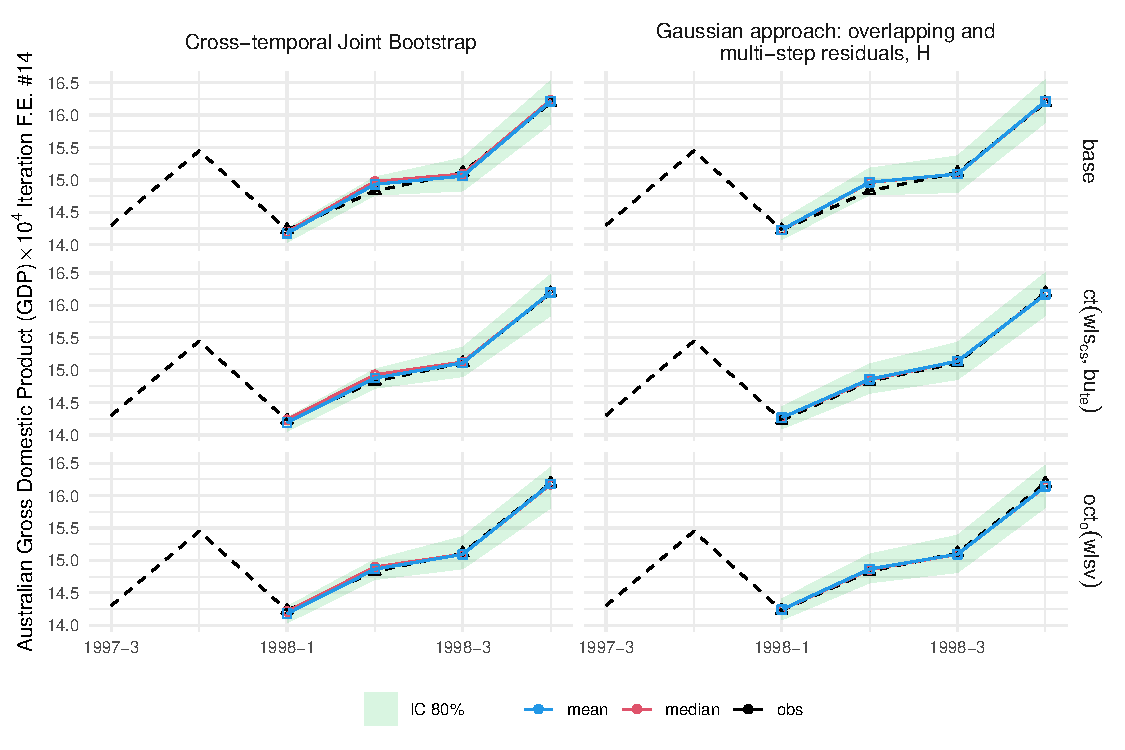
\includegraphics[width = 1\linewidth]{fig/AusGDP/gdptrace14.pdf}
\caption{Base (first row) and reconciled (second and third rows) forecasts for Australian GDP at the second iteration of our forecasting experiment for the bootstrap (first column) and Gaussian (second column) approaches. The green represents the 80\% confidence interval. The black line and triangle indicate the observed true values, the red line represent the median value, and the blue line represent the mean value.}
\label{fig:gdptrace}
\end{figure}

\begin{figure}[p]
\centering
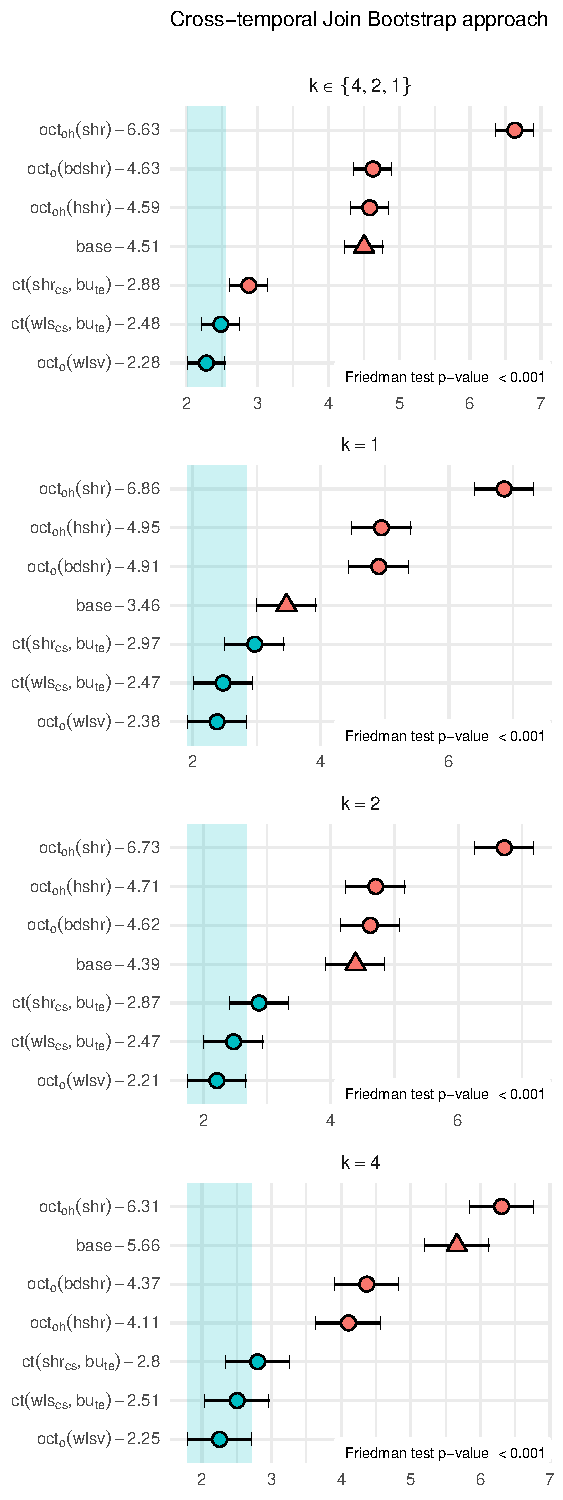
\includegraphics[width = 0.45\linewidth]{fig/AusGDP/ctjb.pdf}
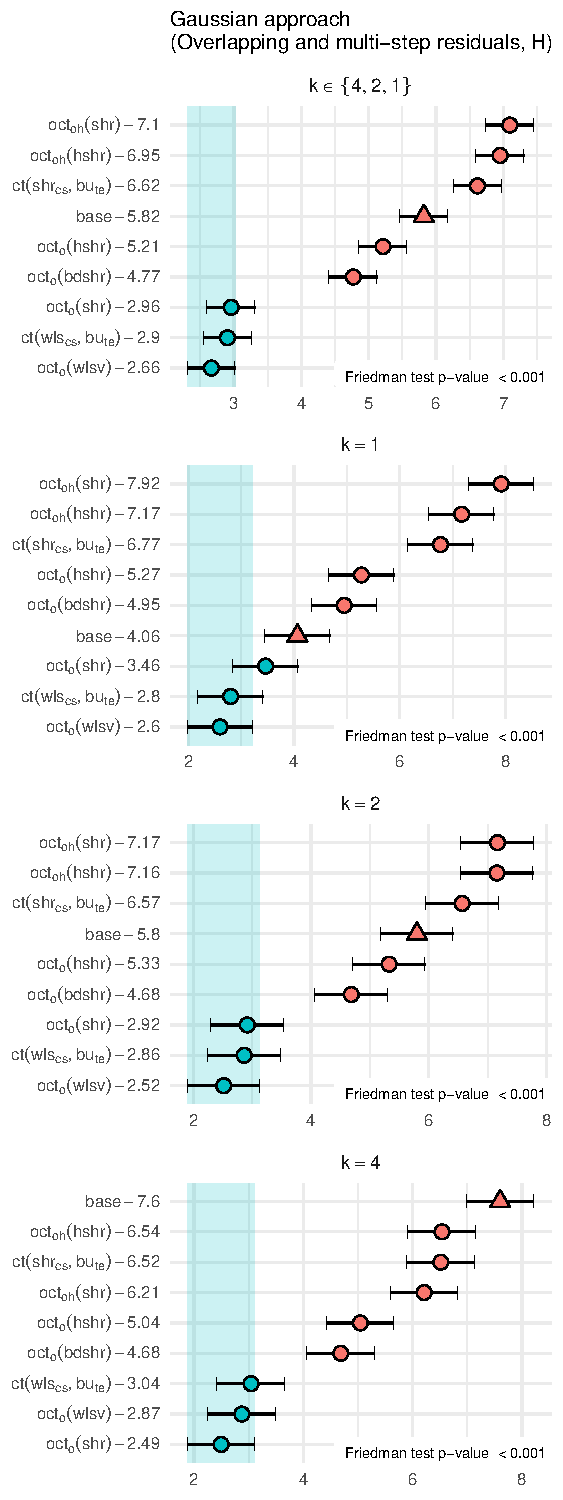
\includegraphics[width = 0.45\linewidth]{fig/AusGDP/hsamoh.pdf}
\caption{“Multiple Comparison with the Best" (MCB) Nemenyi test at different temporal aggregation for the non-parametric bootstrap approach and the Gaussian approach using overlapping and multi-step residuals, with the covariance matrix calculated from the high frequency time series (H). In each panel, the Friedman test is reported in the lower right corner. The mean rank of each approach is shown to the right of its name. Statistical differences in performance were indicated if the intervals of two forecast reconciliation procedures did not overlap. Thus, approaches that did not overlap with the blue interval were considered significantly worse than the best, and vice versa.}
\label{fig:mcb}
\end{figure}

Figure \ref{fig:gdptrace} shows the base (first row) and reconciled (second and third rows) forecasts for Australian GDP at the second iteration of our forecasting experiment for the bootstrap and Gaussian approaches in the first and second columns respectively. The green shading represents the 80\% confidence interval, while the black line with the triangle represents the observed true values. The red line and dot represent the median value, and the blue line and dot represent the mean value. In the nonparametric case, the median and mean are not always overlapped and centered within the confidence interval (asymmetrical), as is the case in the Gaussian distribution. This is because the nonparametric case does not assume a specific underlying distribution for the data.

Figure \ref{fig:mcb} compare the MCB using the CRPS for the non-parametric bootstrap approach and the Gaussian approach using overlapping and multi-step residuals, with the covariance matrix calculated from the matrix of high frequency time series (H). Also in this case, ct$(wls_{cs},bu_{te})$ and oct$_o(wlsv)$ were found to be significantly better than base forecasts at any level of aggregation, and for $k>1$, oct$_{o}(shr)$ also performed similarly to the first two in the Gaussian framework.

Overall, we found that using overlapping residuals almost always leads to a greater improvement in terms of ES and CRPS, and this is also generally true for reconciliation. Forecasts at the most aggregated level (year) seem to benefit the most from reconciliation, and using in-sample residuals with overlapping appears to be sufficient to improve forecasts if the base forecasts take into account the multi-step structure.

\section{Australian Tourism Demand dataset}\label{sec:vn525}

The Australian Tourist Flows (Visitors Night, VN) dataset \citep{wickramasuriya2019, wickramasuriya2020} measures the number of tourists arriving and spending nights in tourist facilities. It includes 228 monthly observations from January 1998 to December 2016, and has a cross-sectional clustered structure based on a geographic hierarchy and a disaggregation by purpose of travel. The geographic hierarchy is divided into seven states, 27 zones of states, and 76 regions of zones, for a total of 111 geographic divisions. However, six of these zones (see Table \ref{tab:australia} in the Appendix \ref{app:australia}) are each formed by a single region, resulting in a total of 105 unique nodes in the hierarchy. The purpose of travel is divided into four categories: holiday (Hol), visiting friends and relatives (Vis), business (Bus), and other (Oth). According to \cite{difonzo2022a}, 24 nodes should not be considered, resulting in an unbalanced hierarchy of 525 unique nodes, referred to as VN525, instead of the theoretical 555. The dataset includes 304 most disaggregated variables, which can be aggregated into 221 upper time series for a total of 525 variables. Table \ref{tab:nseries}  does not include duplicated entries and updates the information in Table 7 from \cite{wickramasuriya2019}. This data can be temporally aggregated into 2, 3, 4, 6, or 12 months ($\mathcal{K} = \{1,2,3,4,6,12\}$).

\begin{table}[tbp]
\spacingset{1.1}
	\centering
	\begin{tabular}{c|cc|c}
		\toprule
		& \multicolumn{3}{c}{\textbf{Number of series}} \\
		& \textbf{G.D.} & \textbf{P.O.T} & Tot.\\
		%& \textbf{division} & \textbf{travel} & \textbf{Total} \\
		\midrule
		Australia & 1 & 4 & 5\\
		States & 7 & 28 & 35\\
		Zones$^*$ & 21 & 84 & 105\\
		Regions & 76 & 304 & 380\\
		\bottomrule
		\textbf{Total} & \textbf{105} & \textbf{420} & \textbf{525}\\
		\bottomrule
		\addlinespace[0.3em]
		\multicolumn{4}{l}{\parbox{7cm}{\footnotesize \textbf{*} 6 Zones with only one Region are included in Regions.}}
	\end{tabular}
	\caption{\label{tab:nseries} Grouped time series for Australian tourism flows.}
\end{table}

The forecasting experiment involves using a recursive training sample with an expanding window length. The process begins by using the first 10 years of data, from January 1998 to December 2008, to make forecasts for the entire following year (2009). Then, the training set is increased by one month and used to forecast the next 12 months, repeating this process until the last training set is used (January 1998 to December 2015). This results in a total of 85 different forecast origins, with each one being replicated in the forecasting experiment. Additionally, forecasts are computed up to 6 steps ahead for time series aggregated over 2 months, up to 4 steps ahead for those aggregated over 3 months, up to 3 steps ahead for those aggregated over 4 months, up to 2 steps ahead for those aggregated over 6 months, and one step ahead for those aggregated over 12 months. ETS models (minimizing the AICc criterion with the \textsf{R} package \texttt{forecast}) are fitted to the log-transformed data, with the resulting base forecasts being back-transformed to produce non-negative forecasts, as described in \cite{wickramasuriya2020}.

\subsection{Base and reconciled samples}\label{ssec:vn_br}

To calculate the base forecasts sample, we use the cross-temporal joint bootstrap method described in Section \ref{ssec:boot} for the nonparametric framework. In the Gaussian scenario, we utilize all four covariance matrices outlined in section \ref{sec:shrtech} with $\lambda=0$ (sample covariance matrix): the \textit{Global} (G), \textit{High frequency} (H), \textit{Bottom time series} (B) and \textit{High frequency Bottom time series} (HB) sample covariance matrices. To compute these matrices, we use multi-step residuals to accurately assess the temporal and cross-sectional relationships, but do not include overlapping, as we are unable to correctly determine the residuals for the overlapping series using ETS models (see Section \ref{ssec:over_res}).

To reconciled the 1000 base forecast samples, we have implemented the following approaches:
\begin{itemize}[nosep, leftmargin = 2.5cm]
	\item[\textbf{ct}$(bu)$] cross-temporal bottom up (see Section \ref{ssec:ctbu});
	\item[\textbf{ct}$(\;\cdot\;, bu_{te})$] partly bottom-up (Section \ref{ssec:ctbu}) starting from cross-sectionally reconciled forecasts using the $shr$ approach (Table \ref{tab:cov_app});
	\item[\textbf{ct}$(\;\cdot\;, bu_{cs})$] partly bottom-up (Section \ref{ssec:ctbu}) starting from temporally reconciled forecasts using the $wlsv$ approach (Table \ref{tab:cov_app});
	\item[\textbf{oct}$(\;\cdot\;)$] optimal cross-temporal reconciliation for the $ols$, $struc$, $wlsv$ and $bdshr$ approach (see Section \ref{ssec:oct}). When necessary ($wlsv$ and $bdshr$), in-sample residuals were used.;
	\item[\textbf{oct}$_{h}(\;\cdot\;)$] optimal cross-temporal reconciliation with multi-step residuals (see Section \ref{ssec:multi_res}) for the shrinkage approaches presented in Section \ref{sec:shrtech}: $shr$ stand for \textit{Global shrinkage}, $hshr$ for \textit{High frequency shrinkage}, $bshr$ for \textit{bottom time series shrinkage}, $hbshr$ for \textit{High frequency bottom time series shrinkage}.
\end{itemize}
One issue in working with time series data is the presence of negative values, which can cause difficulties for certain types of models or analyses.
For the base forecasts, using the bootstrap approach forecasts are naturally non negative (ETS model with the log-transformation), while this is not true for the Gaussian approach. In this case, to satisfy the constraint, we simply set negative values to zero. For the cross-temporal reconciliation, \citet{difonzo2023} offer two potential solutions: a state-of-the-art numerical optimization procedure like \texttt{osqp} (\citealp{stellato2019, stellato2020}) and a simple heuristic strategy called set-negative-to-zero (sntz). In the sntz approach, possible negative values of the reconciled high frequency bottom time series forecasts without any non-negativity constraints are set to zero and finally a cross-temporal reconciliation bottom-up (see Section \ref{ssec:ctbu}) is used to obtain the complete cross-temporal forecasts. \cite{difonzo2023a} found that both methods produced similar quality forecasts for the photovoltaic power generation dataset, but the optimization method required much more time and effort compared to the heuristic method. To reduce computational demands, we chose to use the less time-intensive heuristic approach for reconciliation. Following Theorem \ref{thm:rs}, we are able to obtain the reconciled sample respecting non-negativity constraints starting from an incoherent sample simulated from a normal.

Finally, to evaluate the performance, we employed the Continuous Ranked Probability Score (CRPS), the Energy Score (ES), and “Multiple Comparison with the Best" (MCB) Nemenyi test. These were introduced and discussed in Sections \ref{ssec:acc_scores} and \ref{ssec:aus_br}. %We use the bootstrap base forecasts as benchmark ($s=0$ and $j=0$) for the scores (\ref{eq:skill}), (\ref{eq:skillCRPS_all}), and (\ref{eq:skillES_all})

\subsection{Results}

\begin{table}[p]
\centering
\begingroup
\spacingset{1}
\fontsize{9}{10}\selectfont

\begin{tabular}[t]{l|>{}cccc>{}c|ccccc}
\toprule
\multicolumn{1}{c}{\textbf{}} & \multicolumn{10}{c}{\textbf{Generation of the base forecasts paths}} \\
\cmidrule(l{0pt}r{0pt}){2-11}
\multicolumn{1}{c}{\makecell[c]{\bfseries Reconciliation\\\bfseries approach}} & \multicolumn{1}{c}{ctjb} & \multicolumn{4}{c}{\makecell[c]{Gaussian approach\textsuperscript{*}}} & \multicolumn{1}{c}{ctjb} & \multicolumn{4}{c}{\makecell[c]{Gaussian approach\textsuperscript{*}}} \\
\multicolumn{1}{c}{} &  & G & B & H & \multicolumn{1}{c}{HB} &  & G & B & H & HB\\
\midrule
\addlinespace[0.3em]
\multicolumn{1}{c}{} & \multicolumn{5}{c}{\textbf{$\forall k \in \{12,6,4,3,2,1\}$}} & \multicolumn{5}{c}{\textbf{$k = 1$}}\\
base & \textcolor{black}{1.000} & \textcolor{black}{0.971} & \textcolor{black}{0.971} & \textcolor{black}{0.973} & \textcolor{black}{0.973} & \textcolor{black}{1.000} & \textcolor{black}{0.972} & \textcolor{black}{0.972} & \textcolor{black}{0.972} & \textcolor{black}{0.972}\\
ct$(bu)$ & \textcolor{red}{1.321} & \textcolor{red}{1.011} & \textcolor{red}{1.011} & \textcolor{red}{1.011} & \textcolor{red}{1.011} & \textcolor{red}{1.077} & \textcolor{black}{0.983} & \textcolor{black}{0.982} & \textcolor{black}{0.982} & \textcolor{black}{0.982}\\
ct$(shr_{cs}, bu_{te})$ & \textcolor{red}{1.057} & \textcolor{black}{0.974} & \textcolor{black}{0.969} & \textcolor{black}{0.974} & \textcolor{black}{0.969} & \textcolor{black}{0.976} & \textcolor{black}{0.963} & \textcolor{black}{0.962} & \textcolor{black}{0.963} & \textcolor{black}{0.962}\\
ct$(wlsv_{te}, bu_{cs})$ & \textcolor{red}{1.062} & \textcolor{black}{0.974} & \textcolor{black}{0.974} & \textcolor{black}{0.972} & \textcolor{black}{0.972} & \textcolor{black}{0.976} & \textcolor{black}{0.965} & \textcolor{black}{0.965} & \textcolor{black}{0.966} & \textcolor{black}{0.966}\\
oct$(ols)$ & \textcolor{black}{0.989} & \textcolor{black}{0.989} & \textcolor{black}{0.989} & \textcolor{black}{0.987} & \textcolor{black}{0.987} & \textcolor{black}{0.982} & \textcolor{black}{0.986} & \textcolor{black}{0.988} & \textcolor{black}{0.986} & \textcolor{black}{0.989}\\
oct$(struc)$ & \textcolor{black}{0.982} & \textcolor{black}{0.962} & \textcolor{black}{0.961} & \textcolor{black}{0.961} & \textcolor{black}{0.959} & \textcolor{black}{0.970} & \textcolor{black}{0.963} & \textcolor{black}{0.963} & \textcolor{black}{0.963} & \textcolor{black}{0.963}\\
oct$(wlsv)$ & \textcolor{black}{0.987} & \textcolor{black}{0.959} & \textcolor{black}{0.959} & \textcolor{black}{0.958} & \textcolor{black}{0.957} & \textcolor{black}{0.952} & \textcolor{black}{0.957} & \textcolor{black}{0.957} & \textcolor{black}{0.957} & \textcolor{black}{0.957}\\
oct$(bdshr)$ & \textcolor{black}{0.975} & \textcolor{black}{\textbf{0.956}} & \textcolor{black}{\textbf{0.953}} & \textcolor{black}{\textbf{0.952}} & \textcolor{blue}{\textbf{0.951}} & \textcolor{blue}{\textbf{0.949}} & \textcolor{black}{\textbf{0.955}} & \textcolor{black}{\textbf{0.953}} & \textcolor{black}{\textbf{0.954}} & \textcolor{black}{\textbf{0.954}}\\
oct$_h(hbshr)$ & \textcolor{black}{0.989} & \textcolor{red}{1.018} & \textcolor{red}{1.020} & \textcolor{red}{1.016} & \textcolor{red}{1.018} & \textcolor{black}{0.982} & \textcolor{red}{1.004} & \textcolor{red}{1.007} & \textcolor{red}{1.004} & \textcolor{red}{1.009}\\
oct$_h(bshr)$ & \textcolor{black}{0.994} & \textcolor{red}{1.018} & \textcolor{red}{1.020} & \textcolor{red}{1.016} & \textcolor{red}{1.019} & \textcolor{black}{0.988} & \textcolor{red}{1.007} & \textcolor{red}{1.013} & \textcolor{red}{1.006} & \textcolor{red}{1.012}\\
oct$_h(hshr)$ & \textcolor{black}{\textbf{0.969}} & \textcolor{black}{0.993} & \textcolor{black}{0.993} & \textcolor{black}{0.990} & \textcolor{black}{0.991} & \textcolor{black}{0.953} & \textcolor{black}{0.977} & \textcolor{black}{0.977} & \textcolor{black}{0.979} & \textcolor{black}{0.979}\\
oct$_h(shr)$ & \textcolor{red}{1.007} & \textcolor{black}{0.980} & \textcolor{black}{0.972} & \textcolor{black}{0.970} & \textcolor{black}{0.970} & \textcolor{red}{1.000} & \textcolor{black}{0.986} & \textcolor{black}{0.977} & \textcolor{black}{0.976} & \textcolor{black}{0.974}\\
\addlinespace[0.3em]
\multicolumn{1}{c}{} & \multicolumn{5}{c}{\textbf{$k = 2$}} & \multicolumn{5}{c}{\textbf{$k = 3$}}\\
base & \textcolor{black}{1.000} & \textcolor{black}{0.970} & \textcolor{black}{0.969} & \textcolor{black}{0.970} & \textcolor{black}{0.971} & \textcolor{black}{1.000} & \textcolor{black}{0.971} & \textcolor{black}{0.971} & \textcolor{black}{0.972} & \textcolor{black}{0.973}\\
ct$(bu)$ & \textcolor{red}{1.189} & \textcolor{black}{0.999} & \textcolor{black}{0.999} & \textcolor{black}{0.999} & \textcolor{black}{0.999} & \textcolor{red}{1.273} & \textcolor{red}{1.010} & \textcolor{red}{1.010} & \textcolor{red}{1.010} & \textcolor{red}{1.010}\\
ct$(shr_{cs}, bu_{te})$ & \textcolor{red}{1.015} & \textcolor{black}{0.972} & \textcolor{black}{0.970} & \textcolor{black}{0.972} & \textcolor{black}{0.970} & \textcolor{red}{1.041} & \textcolor{black}{0.977} & \textcolor{black}{0.974} & \textcolor{black}{0.977} & \textcolor{black}{0.974}\\
ct$(wlsv_{te}, bu_{cs})$ & \textcolor{red}{1.016} & \textcolor{black}{0.971} & \textcolor{black}{0.971} & \textcolor{black}{0.970} & \textcolor{black}{0.970} & \textcolor{red}{1.046} & \textcolor{black}{0.976} & \textcolor{black}{0.976} & \textcolor{black}{0.974} & \textcolor{black}{0.974}\\
oct$(ols)$ & \textcolor{black}{0.992} & \textcolor{black}{0.991} & \textcolor{black}{0.991} & \textcolor{black}{0.990} & \textcolor{black}{0.991} & \textcolor{black}{0.994} & \textcolor{black}{0.992} & \textcolor{black}{0.993} & \textcolor{black}{0.991} & \textcolor{black}{0.992}\\
oct$(struc)$ & \textcolor{black}{0.982} & \textcolor{black}{0.966} & \textcolor{black}{0.965} & \textcolor{black}{0.965} & \textcolor{black}{0.965} & \textcolor{black}{0.986} & \textcolor{black}{0.967} & \textcolor{black}{0.966} & \textcolor{black}{0.966} & \textcolor{black}{0.965}\\
oct$(wlsv)$ & \textcolor{black}{0.972} & \textcolor{black}{0.961} & \textcolor{black}{0.960} & \textcolor{black}{0.960} & \textcolor{black}{0.960} & \textcolor{black}{0.983} & \textcolor{black}{0.963} & \textcolor{black}{0.962} & \textcolor{black}{0.962} & \textcolor{black}{0.962}\\
oct$(bdshr)$ & \textcolor{black}{\textbf{0.964}} & \textcolor{black}{\textbf{0.958}} & \textcolor{black}{\textbf{0.957}} & \textcolor{black}{\textbf{0.956}} & \textcolor{blue}{\textbf{0.956}} & \textcolor{black}{0.972} & \textcolor{black}{\textbf{0.960}} & \textcolor{black}{\textbf{0.958}} & \textcolor{black}{\textbf{0.957}} & \textcolor{blue}{\textbf{0.957}}\\
oct$_h(hbshr)$ & \textcolor{black}{0.992} & \textcolor{red}{1.013} & \textcolor{red}{1.015} & \textcolor{red}{1.012} & \textcolor{red}{1.015} & \textcolor{black}{0.994} & \textcolor{red}{1.019} & \textcolor{red}{1.021} & \textcolor{red}{1.018} & \textcolor{red}{1.020}\\
oct$_h(bshr)$ & \textcolor{black}{0.997} & \textcolor{red}{1.015} & \textcolor{red}{1.018} & \textcolor{red}{1.013} & \textcolor{red}{1.017} & \textcolor{black}{0.999} & \textcolor{red}{1.021} & \textcolor{red}{1.022} & \textcolor{red}{1.018} & \textcolor{red}{1.022}\\
oct$_h(hshr)$ & \textcolor{black}{0.965} & \textcolor{black}{0.987} & \textcolor{black}{0.987} & \textcolor{black}{0.986} & \textcolor{black}{0.987} & \textcolor{black}{\textbf{0.971}} & \textcolor{black}{0.994} & \textcolor{black}{0.994} & \textcolor{black}{0.992} & \textcolor{black}{0.993}\\
oct$_h(shr)$ & \textcolor{red}{1.005} & \textcolor{black}{0.986} & \textcolor{black}{0.978} & \textcolor{black}{0.976} & \textcolor{black}{0.975} & \textcolor{red}{1.009} & \textcolor{black}{0.986} & \textcolor{black}{0.978} & \textcolor{black}{0.976} & \textcolor{black}{0.976}\\
\addlinespace[0.3em]
\multicolumn{1}{c}{} & \multicolumn{5}{c}{\textbf{$k = 4$}} & \multicolumn{5}{c}{\textbf{$k = 6$}}\\
base & \textcolor{black}{1.000} & \textcolor{black}{0.973} & \textcolor{black}{0.973} & \textcolor{black}{0.974} & \textcolor{black}{0.975} & \textcolor{black}{1.000} & \textcolor{black}{0.976} & \textcolor{black}{0.976} & \textcolor{black}{0.978} & \textcolor{black}{0.978}\\
ct$(bu)$ & \textcolor{red}{1.340} & \textcolor{red}{1.016} & \textcolor{red}{1.015} & \textcolor{red}{1.015} & \textcolor{red}{1.015} & \textcolor{red}{1.450} & \textcolor{red}{1.023} & \textcolor{red}{1.023} & \textcolor{red}{1.023} & \textcolor{red}{1.023}\\
ct$(shr_{cs}, bu_{te})$ & \textcolor{red}{1.061} & \textcolor{black}{0.978} & \textcolor{black}{0.973} & \textcolor{black}{0.978} & \textcolor{black}{0.973} & \textcolor{red}{1.094} & \textcolor{black}{0.978} & \textcolor{black}{0.972} & \textcolor{black}{0.978} & \textcolor{black}{0.972}\\
ct$(wlsv_{te}, bu_{cs})$ & \textcolor{red}{1.068} & \textcolor{black}{0.977} & \textcolor{black}{0.977} & \textcolor{black}{0.974} & \textcolor{black}{0.974} & \textcolor{red}{1.103} & \textcolor{black}{0.977} & \textcolor{black}{0.977} & \textcolor{black}{0.974} & \textcolor{black}{0.974}\\
oct$(ols)$ & \textcolor{black}{0.993} & \textcolor{black}{0.991} & \textcolor{black}{0.992} & \textcolor{black}{0.990} & \textcolor{black}{0.990} & \textcolor{black}{0.989} & \textcolor{black}{0.989} & \textcolor{black}{0.989} & \textcolor{black}{0.987} & \textcolor{black}{0.986}\\
oct$(struc)$ & \textcolor{black}{0.986} & \textcolor{black}{0.965} & \textcolor{black}{0.964} & \textcolor{black}{0.964} & \textcolor{black}{0.963} & \textcolor{black}{0.986} & \textcolor{black}{0.961} & \textcolor{black}{0.960} & \textcolor{black}{0.959} & \textcolor{black}{0.957}\\
oct$(wlsv)$ & \textcolor{black}{0.990} & \textcolor{black}{0.962} & \textcolor{black}{0.961} & \textcolor{black}{0.961} & \textcolor{black}{0.960} & \textcolor{red}{1.001} & \textcolor{black}{0.960} & \textcolor{black}{0.959} & \textcolor{black}{0.958} & \textcolor{black}{0.957}\\
oct$(bdshr)$ & \textcolor{black}{0.977} & \textcolor{black}{\textbf{0.959}} & \textcolor{black}{\textbf{0.956}} & \textcolor{black}{\textbf{0.955}} & \textcolor{blue}{\textbf{0.954}} & \textcolor{black}{0.985} & \textcolor{black}{\textbf{0.956}} & \textcolor{black}{\textbf{0.953}} & \textcolor{black}{\textbf{0.950}} & \textcolor{blue}{\textbf{0.948}}\\
oct$_h(hbshr)$ & \textcolor{black}{0.993} & \textcolor{red}{1.021} & \textcolor{red}{1.023} & \textcolor{red}{1.019} & \textcolor{red}{1.021} & \textcolor{black}{0.989} & \textcolor{red}{1.024} & \textcolor{red}{1.026} & \textcolor{red}{1.022} & \textcolor{red}{1.022}\\
oct$_h(bshr)$ & \textcolor{black}{0.997} & \textcolor{red}{1.022} & \textcolor{red}{1.022} & \textcolor{red}{1.019} & \textcolor{red}{1.022} & \textcolor{black}{0.994} & \textcolor{red}{1.022} & \textcolor{red}{1.022} & \textcolor{red}{1.020} & \textcolor{red}{1.022}\\
oct$_h(hshr)$ & \textcolor{black}{\textbf{0.973}} & \textcolor{black}{0.996} & \textcolor{black}{0.997} & \textcolor{black}{0.994} & \textcolor{black}{0.995} & \textcolor{black}{\textbf{0.976}} & \textcolor{black}{1.000} & \textcolor{red}{1.001} & \textcolor{black}{0.996} & \textcolor{black}{0.997}\\
oct$_h(shr)$ & \textcolor{red}{1.009} & \textcolor{black}{0.984} & \textcolor{black}{0.976} & \textcolor{black}{0.973} & \textcolor{black}{0.973} & \textcolor{red}{1.010} & \textcolor{black}{0.978} & \textcolor{black}{0.970} & \textcolor{black}{0.967} & \textcolor{black}{0.967}\\
\addlinespace[0.3em]
\multicolumn{1}{c}{} & \multicolumn{5}{c}{\textbf{$k = 12$}} & \multicolumn{5}{c}{}\\
base & \textcolor{black}{1.000} & \textcolor{black}{0.968} & \textcolor{black}{0.967} & \textcolor{black}{0.969} & \textcolor{black}{0.969} &  &  &  &  & \\
ct$(bu)$ & \textcolor{red}{1.675} & \textcolor{red}{1.038} & \textcolor{red}{1.037} & \textcolor{red}{1.037} & \textcolor{red}{1.038} &  &  &  &  & \\
ct$(shr_{cs}, bu_{te})$ & \textcolor{red}{1.163} & \textcolor{black}{0.977} & \textcolor{black}{0.965} & \textcolor{black}{0.977} & \textcolor{black}{0.965} &  &  &  &  & \\
ct$(wlsv_{te}, bu_{cs})$ & \textcolor{red}{1.174} & \textcolor{black}{0.978} & \textcolor{black}{0.978} & \textcolor{black}{0.971} & \textcolor{black}{0.971} &  &  &  &  & \\
oct$(ols)$ & \textcolor{black}{0.982} & \textcolor{black}{0.982} & \textcolor{black}{0.983} & \textcolor{black}{0.980} & \textcolor{black}{0.975} &  &  &  &  & \\
oct$(struc)$ & \textcolor{black}{0.982} & \textcolor{black}{0.951} & \textcolor{black}{0.949} & \textcolor{black}{0.947} & \textcolor{black}{0.943} &  &  &  &  & \\
oct$(wlsv)$ & \textcolor{red}{1.025} & \textcolor{black}{0.954} & \textcolor{black}{0.953} & \textcolor{black}{0.949} & \textcolor{black}{0.947} &  &  &  &  & \\
oct$(bdshr)$ & \textcolor{red}{1.002} & \textcolor{black}{\textbf{0.950}} & \textcolor{black}{\textbf{0.944}} & \textcolor{black}{\textbf{0.939}} & \textcolor{blue}{\textbf{0.935}} &  &  &  &  & \\
oct$_h(hbshr)$ & \textcolor{black}{0.982} & \textcolor{red}{1.027} & \textcolor{red}{1.029} & \textcolor{red}{1.024} & \textcolor{red}{1.021} &  &  &  &  & \\
oct$_h(bshr)$ & \textcolor{black}{0.987} & \textcolor{red}{1.024} & \textcolor{red}{1.021} & \textcolor{red}{1.021} & \textcolor{red}{1.019} &  &  &  &  & \\
oct$_h(hshr)$ & \textcolor{black}{\textbf{0.978}} & \textcolor{red}{1.003} & \textcolor{red}{1.005} & \textcolor{black}{0.996} & \textcolor{black}{0.997} &  &  &  &  & \\
oct$_h(shr)$ & \textcolor{red}{1.010} & \textcolor{black}{0.963} & \textcolor{black}{0.956} & \textcolor{black}{0.952} & \textcolor{black}{0.952} &  &  &  &  & \\
\bottomrule
\multicolumn{11}{l}{\rule{0pt}{1em}\rule{0pt}{1.75em}\makecell[l]{$^\ast$The Gaussian method employs a sample covariance matrix and includes four techniques\\ (G, B, H, HB) with multi-step residuals.}}\\
\end{tabular}

\endgroup
\caption{CRPS skill score defined in equation (\ref{eq:skill}) and (\ref{eq:skillCRPS_all}) for VN525 dataset. The smaller this value, the more accurate the forecast. Approaches that performed worse than the benchmark model (Bootstrap base forecasts) are highlighted in red, the best for each column is marked in bold, and the overall lowest value is highlighted in blue. The notation used to refer to the reconciliation and base forecast samples is explained in Section \ref{ssec:vn_br}.}
\label{tab:vncrps}
\end{table}

\begin{table}[p]
\centering
\begingroup
\spacingset{1}
\fontsize{9}{10}\selectfont

\begin{tabular}[t]{c|>{}cccc>{}c|ccccc}
\toprule
\multicolumn{1}{c}{\textbf{}} & \multicolumn{10}{c}{\textbf{Base forecasts' sample approach}} \\
\cmidrule(l{0pt}r{0pt}){2-11}
\multicolumn{1}{c}{\makecell[c]{\bfseries Reconciliation\\\bfseries approach}} & \multicolumn{1}{c}{ctjb} & \multicolumn{4}{c}{\makecell[c]{Gaussian approach\textsuperscript{*}}} & \multicolumn{1}{c}{ctjb} & \multicolumn{4}{c}{\makecell[c]{Gaussian approach\textsuperscript{*}}} \\
\multicolumn{1}{c}{} &  & G & B & H & \multicolumn{1}{c}{HB} &  & G & B & H & HB\\
\midrule
\addlinespace[0.3em]
\multicolumn{1}{c}{} & \multicolumn{5}{c}{\textbf{$\forall k \in \{12,6,4,3,2,1\}$}} & \multicolumn{5}{c}{\textbf{$k = 1$}}\\
base & \textcolor{black}{1.000} & \textcolor{black}{0.956} & \textcolor{black}{0.955} & \textcolor{black}{0.958} & \textcolor{black}{0.951} & \textcolor{black}{1.000} & \textcolor{black}{0.952} & \textcolor{black}{0.950} & \textcolor{black}{0.952} & \textcolor{black}{0.950}\\
ct$(bu)$ & \textcolor{red}{2.427} & \textcolor{black}{0.983} & \textcolor{black}{0.983} & \textcolor{black}{0.983} & \textcolor{black}{0.983} & \textcolor{red}{1.759} & \textcolor{black}{0.982} & \textcolor{black}{0.982} & \textcolor{black}{0.982} & \textcolor{black}{0.982}\\
ct$(shr_{cs}, bu_{te})$ & \textcolor{red}{1.243} & \textcolor{black}{0.886} & \textcolor{black}{0.879} & \textcolor{black}{0.886} & \textcolor{black}{0.879} & \textcolor{red}{1.098} & \textcolor{black}{0.929} & \textcolor{black}{0.928} & \textcolor{black}{0.930} & \textcolor{black}{0.927}\\
ct$(wlsv_{te}, bu_{cs})$ & \textcolor{red}{1.499} & \textcolor{black}{0.977} & \textcolor{black}{0.977} & \textcolor{black}{0.971} & \textcolor{black}{0.972} & \textcolor{red}{1.241} & \textcolor{black}{0.975} & \textcolor{black}{0.975} & \textcolor{black}{0.973} & \textcolor{black}{0.974}\\
oct$(ols)$ & \textcolor{black}{0.955} & \textcolor{black}{0.893} & \textcolor{black}{0.891} & \textcolor{black}{0.893} & \textcolor{black}{0.888} & \textcolor{black}{0.975} & \textcolor{black}{0.937} & \textcolor{black}{0.936} & \textcolor{black}{0.936} & \textcolor{black}{0.935}\\
oct$(struc)$ & \textcolor{red}{1.085} & \textcolor{black}{0.917} & \textcolor{black}{0.915} & \textcolor{black}{0.916} & \textcolor{black}{0.912} & \textcolor{red}{1.027} & \textcolor{black}{0.943} & \textcolor{black}{0.942} & \textcolor{black}{0.943} & \textcolor{black}{0.942}\\
oct$(wlsv)$ & \textcolor{red}{1.132} & \textcolor{black}{0.933} & \textcolor{black}{0.929} & \textcolor{black}{0.931} & \textcolor{black}{0.927} & \textcolor{red}{1.050} & \textcolor{black}{0.951} & \textcolor{black}{0.949} & \textcolor{black}{0.950} & \textcolor{black}{0.949}\\
oct$(bdshr)$ & \textcolor{red}{1.047} & \textcolor{black}{0.904} & \textcolor{black}{0.897} & \textcolor{black}{0.897} & \textcolor{black}{0.891} & \textcolor{red}{1.009} & \textcolor{black}{0.936} & \textcolor{black}{0.933} & \textcolor{black}{0.934} & \textcolor{black}{0.931}\\
oct$_h(hbshr)$ & \textcolor{black}{0.956} & \textcolor{black}{0.889} & \textcolor{black}{0.886} & \textcolor{black}{0.888} & \textcolor{black}{0.884} & \textcolor{black}{0.975} & \textcolor{black}{0.937} & \textcolor{black}{0.936} & \textcolor{black}{0.937} & \textcolor{black}{0.935}\\
oct$_h(bshr)$ & \textcolor{black}{\textbf{0.931}} & \textcolor{black}{\textbf{0.867}} & \textcolor{black}{\textbf{0.866}} & \textcolor{black}{\textbf{0.863}} & \textcolor{blue}{\textbf{0.860}} & \textcolor{black}{\textbf{0.965}} & \textcolor{black}{\textbf{0.927}} & \textcolor{black}{0.927} & \textcolor{black}{0.925} & \textcolor{black}{0.923}\\
oct$_h(hshr)$ & \textcolor{red}{1.081} & \textcolor{black}{0.935} & \textcolor{black}{0.931} & \textcolor{black}{0.935} & \textcolor{black}{0.927} & \textcolor{red}{1.028} & \textcolor{black}{0.952} & \textcolor{black}{0.951} & \textcolor{black}{0.952} & \textcolor{black}{0.950}\\
oct$_h(shr)$ & \textcolor{red}{1.068} & \textcolor{black}{0.899} & \textcolor{black}{0.878} & \textcolor{black}{0.875} & \textcolor{black}{0.864} & \textcolor{red}{1.023} & \textcolor{black}{0.935} & \textcolor{black}{\textbf{0.923}} & \textcolor{black}{\textbf{0.921}} & \textcolor{blue}{\textbf{0.916}}\\
\addlinespace[0.3em]
\multicolumn{1}{c}{} & \multicolumn{5}{c}{\textbf{$k = 2$}} & \multicolumn{5}{c}{\textbf{$k = 3$}}\\
base & \textcolor{black}{1.000} & \textcolor{black}{0.958} & \textcolor{black}{0.954} & \textcolor{black}{0.956} & \textcolor{black}{0.953} & \textcolor{black}{1.000} & \textcolor{black}{0.961} & \textcolor{black}{0.958} & \textcolor{black}{0.960} & \textcolor{black}{0.955}\\
ct$(bu)$ & \textcolor{red}{2.176} & \textcolor{red}{1.001} & \textcolor{red}{1.001} & \textcolor{red}{1.001} & \textcolor{red}{1.001} & \textcolor{red}{2.428} & \textcolor{black}{0.998} & \textcolor{black}{0.997} & \textcolor{black}{0.997} & \textcolor{black}{0.997}\\
ct$(shr_{cs}, bu_{te})$ & \textcolor{red}{1.192} & \textcolor{black}{0.927} & \textcolor{black}{0.921} & \textcolor{black}{0.927} & \textcolor{black}{0.921} & \textcolor{red}{1.245} & \textcolor{black}{0.911} & \textcolor{black}{0.904} & \textcolor{black}{0.911} & \textcolor{black}{0.904}\\
ct$(wlsv_{te}, bu_{cs})$ & \textcolor{red}{1.400} & \textcolor{black}{0.992} & \textcolor{black}{0.992} & \textcolor{black}{0.988} & \textcolor{black}{0.988} & \textcolor{red}{1.500} & \textcolor{black}{0.991} & \textcolor{black}{0.991} & \textcolor{black}{0.986} & \textcolor{black}{0.987}\\
oct$(ols)$ & \textcolor{black}{0.985} & \textcolor{black}{0.935} & \textcolor{black}{0.932} & \textcolor{black}{0.934} & \textcolor{black}{0.930} & \textcolor{black}{0.976} & \textcolor{black}{0.918} & \textcolor{black}{0.915} & \textcolor{black}{0.917} & \textcolor{black}{0.912}\\
oct$(struc)$ & \textcolor{red}{1.075} & \textcolor{black}{0.949} & \textcolor{black}{0.947} & \textcolor{black}{0.948} & \textcolor{black}{0.944} & \textcolor{red}{1.096} & \textcolor{black}{0.939} & \textcolor{black}{0.936} & \textcolor{black}{0.938} & \textcolor{black}{0.933}\\
oct$(wlsv)$ & \textcolor{red}{1.110} & \textcolor{black}{0.960} & \textcolor{black}{0.958} & \textcolor{black}{0.958} & \textcolor{black}{0.955} & \textcolor{red}{1.142} & \textcolor{black}{0.953} & \textcolor{black}{0.949} & \textcolor{black}{0.951} & \textcolor{black}{0.946}\\
oct$(bdshr)$ & \textcolor{red}{1.045} & \textcolor{black}{0.938} & \textcolor{black}{0.933} & \textcolor{black}{0.933} & \textcolor{black}{0.929} & \textcolor{red}{1.060} & \textcolor{black}{0.926} & \textcolor{black}{0.920} & \textcolor{black}{0.921} & \textcolor{black}{0.915}\\
oct$_h(hbshr)$ & \textcolor{black}{0.984} & \textcolor{black}{0.933} & \textcolor{black}{0.931} & \textcolor{black}{0.933} & \textcolor{black}{0.928} & \textcolor{black}{0.975} & \textcolor{black}{0.915} & \textcolor{black}{0.912} & \textcolor{black}{0.915} & \textcolor{black}{0.909}\\
oct$_h(bshr)$ & \textcolor{black}{\textbf{0.967}} & \textcolor{black}{\textbf{0.917}} & \textcolor{black}{\textbf{0.916}} & \textcolor{black}{0.913} & \textcolor{black}{0.908} & \textcolor{black}{\textbf{0.954}} & \textcolor{black}{\textbf{0.895}} & \textcolor{black}{\textbf{0.895}} & \textcolor{black}{\textbf{0.892}} & \textcolor{blue}{\textbf{0.887}}\\
oct$_h(hshr)$ & \textcolor{red}{1.073} & \textcolor{black}{0.962} & \textcolor{black}{0.959} & \textcolor{black}{0.963} & \textcolor{black}{0.956} & \textcolor{red}{1.093} & \textcolor{black}{0.955} & \textcolor{black}{0.951} & \textcolor{black}{0.956} & \textcolor{black}{0.949}\\
oct$_h(shr)$ & \textcolor{red}{1.064} & \textcolor{black}{0.933} & \textcolor{black}{0.916} & \textcolor{black}{\textbf{0.913}} & \textcolor{blue}{\textbf{0.904}} & \textcolor{red}{1.082} & \textcolor{black}{0.923} & \textcolor{black}{0.903} & \textcolor{black}{0.900} & \textcolor{black}{0.890}\\
\addlinespace[0.3em]
\multicolumn{1}{c}{} & \multicolumn{5}{c}{\textbf{$k = 4$}} & \multicolumn{5}{c}{\textbf{$k = 6$}}\\
base & \textcolor{black}{1.000} & \textcolor{black}{0.960} & \textcolor{black}{0.960} & \textcolor{black}{0.962} & \textcolor{black}{0.956} & \textcolor{black}{1.000} & \textcolor{black}{0.961} & \textcolor{black}{0.959} & \textcolor{black}{0.964} & \textcolor{black}{0.956}\\
ct$(bu)$ & \textcolor{red}{2.585} & \textcolor{black}{0.996} & \textcolor{black}{0.996} & \textcolor{black}{0.995} & \textcolor{black}{0.996} & \textcolor{red}{2.849} & \textcolor{red}{1.004} & \textcolor{red}{1.003} & \textcolor{red}{1.003} & \textcolor{red}{1.004}\\
ct$(shr_{cs}, bu_{te})$ & \textcolor{red}{1.277} & \textcolor{black}{0.898} & \textcolor{black}{0.890} & \textcolor{black}{0.899} & \textcolor{black}{0.891} & \textcolor{red}{1.339} & \textcolor{black}{0.882} & \textcolor{black}{0.873} & \textcolor{black}{0.883} & \textcolor{black}{0.874}\\
ct$(wlsv_{te}, bu_{cs})$ & \textcolor{red}{1.559} & \textcolor{black}{0.990} & \textcolor{black}{0.990} & \textcolor{black}{0.984} & \textcolor{black}{0.985} & \textcolor{red}{1.662} & \textcolor{black}{0.997} & \textcolor{black}{0.997} & \textcolor{black}{0.991} & \textcolor{black}{0.992}\\
oct$(ols)$ & \textcolor{black}{0.966} & \textcolor{black}{0.905} & \textcolor{black}{0.902} & \textcolor{black}{0.904} & \textcolor{black}{0.899} & \textcolor{black}{0.962} & \textcolor{black}{0.889} & \textcolor{black}{0.887} & \textcolor{black}{0.890} & \textcolor{black}{0.885}\\
oct$(struc)$ & \textcolor{red}{1.106} & \textcolor{black}{0.930} & \textcolor{black}{0.927} & \textcolor{black}{0.928} & \textcolor{black}{0.924} & \textcolor{red}{1.132} & \textcolor{black}{0.923} & \textcolor{black}{0.919} & \textcolor{black}{0.922} & \textcolor{black}{0.916}\\
oct$(wlsv)$ & \textcolor{red}{1.157} & \textcolor{black}{0.947} & \textcolor{black}{0.943} & \textcolor{black}{0.945} & \textcolor{black}{0.939} & \textcolor{red}{1.192} & \textcolor{black}{0.942} & \textcolor{black}{0.937} & \textcolor{black}{0.941} & \textcolor{black}{0.934}\\
oct$(bdshr)$ & \textcolor{red}{1.065} & \textcolor{black}{0.917} & \textcolor{black}{0.909} & \textcolor{black}{0.910} & \textcolor{black}{0.903} & \textcolor{red}{1.084} & \textcolor{black}{0.907} & \textcolor{black}{0.897} & \textcolor{black}{0.898} & \textcolor{black}{0.890}\\
oct$_h(hbshr)$ & \textcolor{black}{0.967} & \textcolor{black}{0.901} & \textcolor{black}{0.898} & \textcolor{black}{0.900} & \textcolor{black}{0.895} & \textcolor{black}{0.964} & \textcolor{black}{0.882} & \textcolor{black}{0.880} & \textcolor{black}{0.883} & \textcolor{black}{0.877}\\
oct$_h(bshr)$ & \textcolor{black}{\textbf{0.943}} & \textcolor{black}{\textbf{0.879}} & \textcolor{black}{\textbf{0.878}} & \textcolor{black}{\textbf{0.876}} & \textcolor{blue}{\textbf{0.871}} & \textcolor{black}{\textbf{0.932}} & \textcolor{black}{\textbf{0.856}} & \textcolor{black}{\textbf{0.855}} & \textcolor{black}{\textbf{0.851}} & \textcolor{blue}{\textbf{0.848}}\\
oct$_h(hshr)$ & \textcolor{red}{1.101} & \textcolor{black}{0.949} & \textcolor{black}{0.944} & \textcolor{black}{0.949} & \textcolor{black}{0.941} & \textcolor{red}{1.126} & \textcolor{black}{0.945} & \textcolor{black}{0.939} & \textcolor{black}{0.945} & \textcolor{black}{0.936}\\
oct$_h(shr)$ & \textcolor{red}{1.089} & \textcolor{black}{0.915} & \textcolor{black}{0.893} & \textcolor{black}{0.890} & \textcolor{black}{0.878} & \textcolor{red}{1.107} & \textcolor{black}{0.899} & \textcolor{black}{0.875} & \textcolor{black}{0.871} & \textcolor{black}{0.858}\\
\addlinespace[0.3em]
\multicolumn{1}{c}{} & \multicolumn{5}{c}{\textbf{$k = 12$}} & \multicolumn{5}{c}{}\\
base & \textcolor{black}{1.000} & \textcolor{black}{0.942} & \textcolor{black}{0.947} & \textcolor{black}{0.951} & \textcolor{black}{0.937} &  &  &  &  & \\
ct$(bu)$ & \textcolor{red}{2.990} & \textcolor{black}{0.922} & \textcolor{black}{0.921} & \textcolor{black}{0.923} & \textcolor{black}{0.923} &  &  &  &  & \\
ct$(shr_{cs}, bu_{te})$ & \textcolor{red}{1.326} & \textcolor{black}{0.779} & \textcolor{black}{0.767} & \textcolor{black}{0.777} & \textcolor{black}{0.766} &  &  &  &  & \\
ct$(wlsv_{te}, bu_{cs})$ & \textcolor{red}{1.679} & \textcolor{black}{0.917} & \textcolor{black}{0.917} & \textcolor{black}{0.906} & \textcolor{black}{0.908} &  &  &  &  & \\
oct$(ols)$ & \textcolor{black}{0.872} & \textcolor{black}{0.783} & \textcolor{black}{0.784} & \textcolor{black}{0.783} & \textcolor{black}{0.779} &  &  &  &  & \\
oct$(struc)$ & \textcolor{red}{1.077} & \textcolor{black}{0.826} & \textcolor{black}{0.822} & \textcolor{black}{0.823} & \textcolor{black}{0.818} &  &  &  &  & \\
oct$(wlsv)$ & \textcolor{red}{1.149} & \textcolor{black}{0.851} & \textcolor{black}{0.845} & \textcolor{black}{0.847} & \textcolor{black}{0.840} &  &  &  &  & \\
oct$(bdshr)$ & \textcolor{red}{1.021} & \textcolor{black}{0.808} & \textcolor{black}{0.796} & \textcolor{black}{0.796} & \textcolor{black}{0.787} &  &  &  &  & \\
oct$_h(hbshr)$ & \textcolor{black}{0.872} & \textcolor{black}{0.775} & \textcolor{black}{0.772} & \textcolor{black}{0.772} & \textcolor{black}{0.770} &  &  &  &  & \\
oct$_h(bshr)$ & \textcolor{black}{\textbf{0.833}} & \textcolor{black}{\textbf{0.741}} & \textcolor{black}{\textbf{0.741}} & \textcolor{black}{\textbf{0.737}} & \textcolor{blue}{\textbf{0.735}} &  &  &  &  & \\
oct$_h(hshr)$ & \textcolor{red}{1.066} & \textcolor{black}{0.851} & \textcolor{black}{0.846} & \textcolor{black}{0.848} & \textcolor{black}{0.838} &  &  &  &  & \\
oct$_h(shr)$ & \textcolor{red}{1.043} & \textcolor{black}{0.797} & \textcolor{black}{0.768} & \textcolor{black}{0.764} & \textcolor{black}{0.750} &  &  &  &  & \\
\bottomrule
\multicolumn{11}{l}{\rule{0pt}{1em}\rule{0pt}{1.75em}\makecell[l]{$^\ast$The Gaussian method employs a sample covariance matrix and includes four techniques (G, B, H, HB)\\ with multi-step residuals.}}\\
\end{tabular}

\endgroup
\caption{ES skill score defined in equation (\ref{eq:skill}) and (\ref{eq:skillES_all}) for VN525 dataset. The smaller this value, the more accurate the forecast. Approaches that performed worse than the benchmark model (Bootstrap base forecasts) are highlighted in red, the best for each column is marked in bold, and the overall lowest value is highlighted in blue. The notation used to refer to the reconciliation and base forecast samples is explained in Section \ref{ssec:vn_br}.}
\label{tab:vnes}
\end{table}

The skill scores for CRPS and ES are shown in Tables \ref{tab:vncrps} and \ref{tab:vnes}, respectively. These tables are divided by different temporal levels and each column uses a different approach to calculate the base forecasts, referred to as “base". The different reconciliation approaches are indicated by the rows. The bootstrap method was used as a benchmark to calculate the skill scores. The bootstrap method indices were used as a benchmark.

Looking at the base rows of each table, base forecasts using a Gaussian approach are better in terms of both CRPS and ES compared to the bootstrap approach (our benchmark). Assumptions of truncated Gaussianity (Gaussian with negative values set to zero) may seem strict, but given the limited number of residuals, it can lead to improved forecasts in terms of CRPS and ES. This was confirmed also by the results in the GDP application. Bootstrap forecasts suffer from the limited number of residuals available and are unable to provide a detailed understanding of the distribution, leading to lower predictive accuracy. The Gaussian approach overcomes this limitation and provides better results. Regarding the different covariance matrix estimates for Gaussian base forecasts, there are not big differences. For this reason, using only the high frequency bottom time series can be useful to estimate fewer parameters and reduce the initial dimensionality.

In the Gaussian case, bottom up ct$(bu)$ and partly bottom-up techniques like ct$(shr_{cs}, bu_{te})$ and ct$(wlsv_{te}, bu_{cs})$ lead to better results than the benchmark (bootstrap base forecasts). However, it's not always guaranteed that the improvement is higher than the starting base forecasts (by comparing the value of each column). This is particularly true for higher levels of temporal aggregation ($k \in \{12, 6, 4, 3\}$). Overall, oct$(bdshr)$ in terms of CRPS is almost always the best. The shrinkage approach oct$_h(hshr)$ has good performance in the bootstrap case: it is competitive with oct$(bdshr)$ in lower temporal level ($k \in \{1,2\}$) and it is able to improve for $k\ge 3$. In terms of ES, oct$(bdshr)$ still competitive, although it is not always the approach with the best improvement. In this case, approaches that attempt to establish a temporal and cross-sectional relationship, such as oct$_h(hbshr)$ and oct$_h(bshr)$, are better. %The difference in performance is due to the nature of the calculation of the indices (see Section \ref{ssec:acc_scores}).
It is also worth noting that techniques that don't make use of residuals like oct$(ols)$ and oct$(struc)$ prove to be competitive by consistently improving the base forecasts in terms of CRPS and ES.

Figure \ref{fig:vnmcb_ctjb} and \ref{fig:vnmcb_h} show the MCB using the CRPS for the non-parametric bootstrap approach and the Gaussian approach using multi-step residuals (HB). In general, partly bottom-up procedure improves with respect to base forecasts at monthly level, but optimal cross-temporal procedures are always better. In the bootstrap framework, we can identify a group of three procedure, oct$(bdshr)$, oct$(hshr)$ and oct$(struc)$ that are almost always in the group of the best approaches (underlying with the blue dot). In the Gaussian framework, oct$(wlsv)$, oct$(struc)$, and oct$(bdshr)$ are always significantly better than base forecasts and equivalent in terms of results for temporal aggregation orders greater than 2. For monthly series, oct$(bdshr)$ is always significantly better than all other approaches.

\begin{figure}[p]
\centering
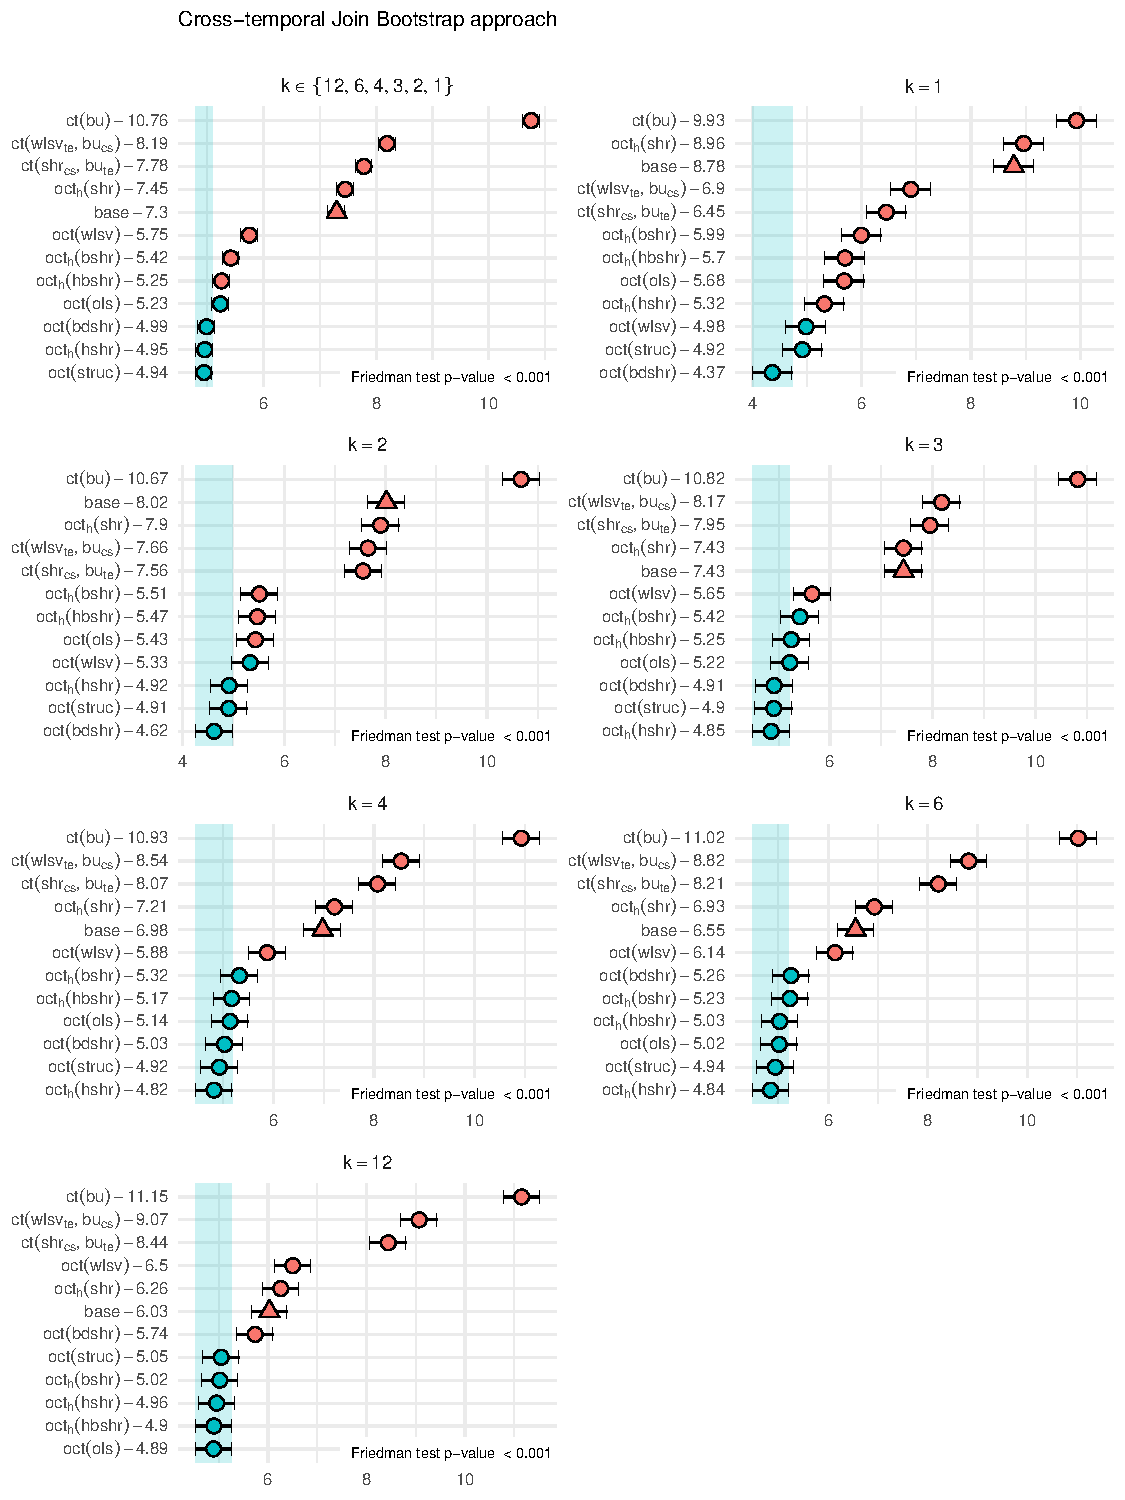
\includegraphics[width = 0.95\linewidth]{fig/VN525/ctjb_more.pdf}
\caption{“Multiple Comparison with the Best" (MCB) Nemenyi test at different temporal aggregation for the non-parametric bootstrap approach. In each panel, the Friedman test is reported in the lower right corner. The mean rank of each approach is shown to the right of its name. Statistical differences in performance were indicated if the intervals of two forecast reconciliation procedures did not overlap. Thus, approaches that did not overlap with the blue interval were considered significantly worse than the best, and vice versa.}
\label{fig:vnmcb_ctjb}
\end{figure}

\begin{figure}[p]
\centering
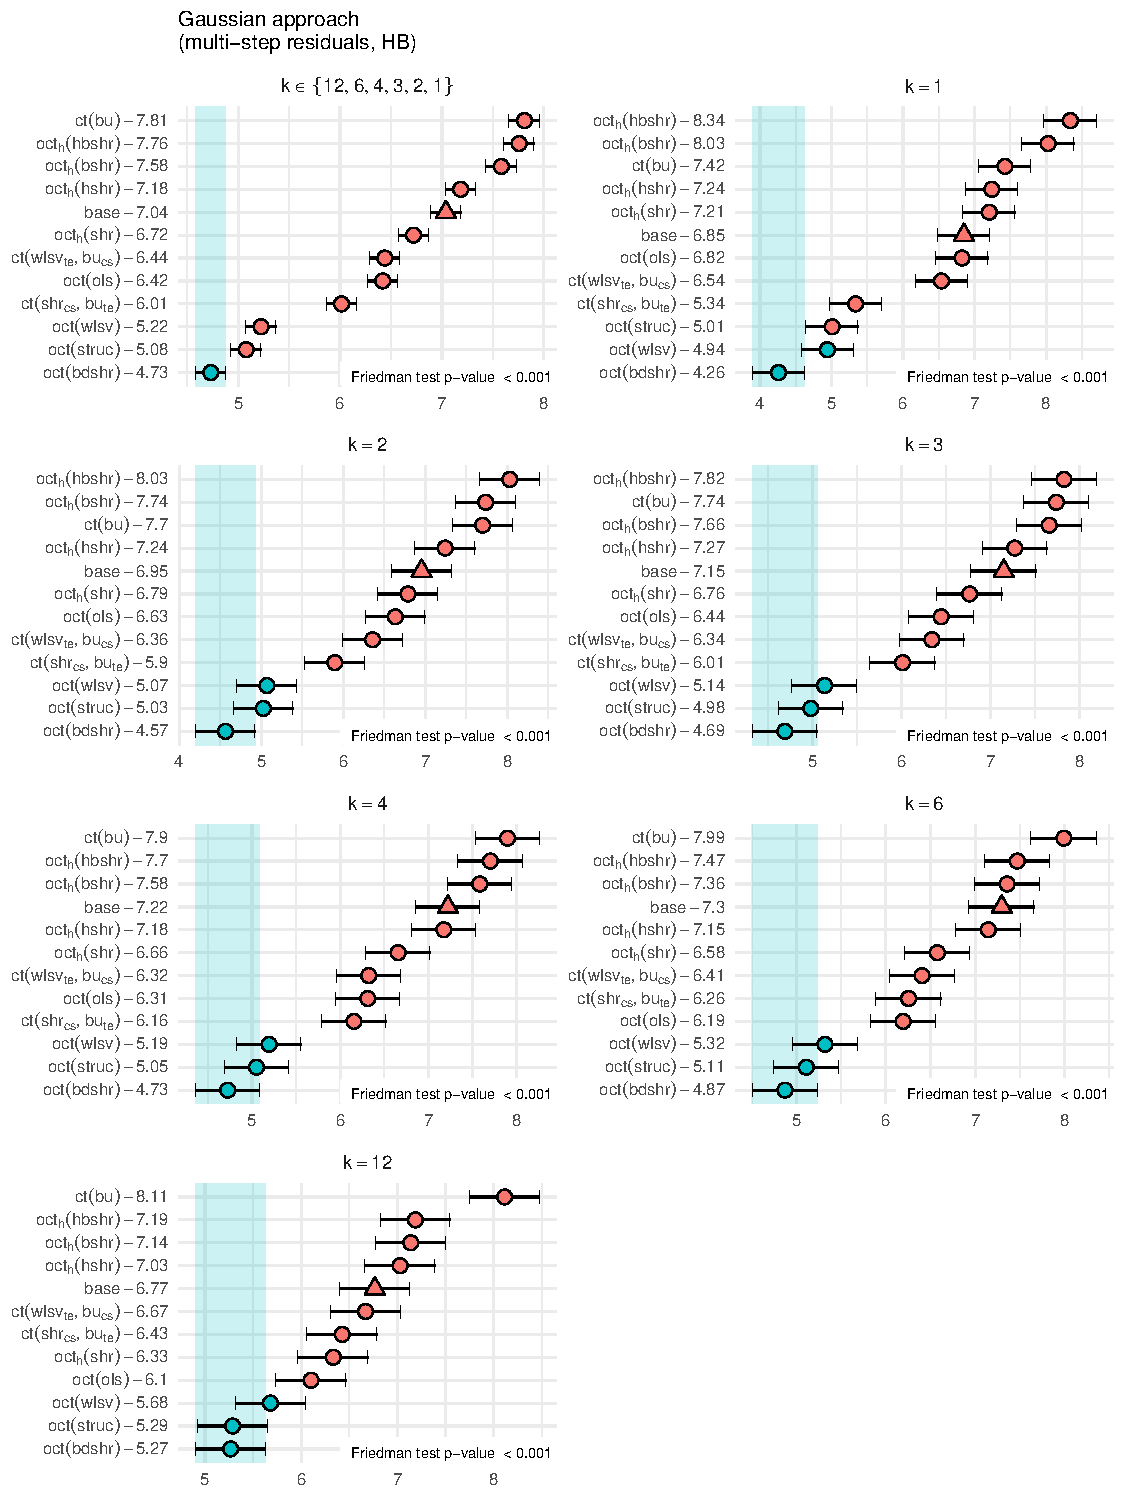
\includegraphics[width = \linewidth]{fig/VN525/hbsamh_more.pdf}
\caption{“Multiple Comparison with the Best" (MCB) Nemenyi test at different temporal aggregation for the Gaussian approach using multi-step residuals, with the covariance matrix calculated from high frequency bottom time series (HB). In each panel, the Friedman test is reported in the lower right corner. The mean rank of each approach is shown to the right of its name. Statistical differences in performance were indicated if the intervals of two forecast reconciliation procedures did not overlap. Thus, approaches that did not overlap with the blue interval were considered significantly worse than the best, and vice versa.}
\label{fig:vnmcb_h}
\end{figure}

\section{Conclusion}\label{sec:conclusion}
In this paper, we extend the probabilistic reconciliation results proposed by \cite{panagiotelis2023} to the cross-temporal case. Through an appropriate use of the notation we show how theorems and definitions valid for the cross-sectional case can be reinterpreted. We propose a bootstrap approach to simulate the base forecasts able to capturing both temporal and cross-temporal relationships simultaneously, and we extend the results under Gaussian assumptions. This work opens the way for further research into the cross-temporal probabilistic forecasting field. The notation proposed can help to investigate extensions following different probabilistic approaches, like in \cite{jeon2019}, \cite{bentaieb2021} and \cite{corani2022}.

Moreover, we analyzed the use of residuals, showing that in-sample residuals fail to capture the temporal structure and we proposed multi-step residuals that can fully capture the full cross-temporal relationships. When dealing with covariance matrices (due to the high-dimension), we proposed four alternative forms to reduce the number of parameters to be estimated. The overlapping residuals try to address the high-dimension problem and require further investigation in future works. We presented a simple simulation to clarify what happens in cross-temporal cases using different types of residuals.% from both an empirical and theoretical perspective.

Finally, we performed two empirical analysis on two classical data set for the forecast reconciliation research field: the Australian GDP, and the Australian Tourism Demand. We found that optimal cross-temporal reconciliation techniques are significantly better then base forecasts. We also compared them with partly bottom-up techniques that use uni-dimensional reconciliations (either cross-sectional or temporal) and found that they perform better, especially at higher levels of temporal aggregation. All the reconciliation methods proposed are available in \textsf{R} package \texttt{FoReco} \citep{girolimetto2022}. In conclusion, reconciliation approaches can play an important role to improve the accuracy of forecasts also in a probabilistic framework.

\section*{Acknowledgements}
\noindent Tommaso Di Fonzo and Daniele Girolimetto acknowledge financial support from project PRIN2017 “HiDEA: Advanced Econometrics for High-frequency Data”, 2017RSMPZZ. Rob Hyndman acknowledges the support of the Australian Government through the Australian Research Council Industrial Transformation Training Centre in Optimisation Technologies, Integrated Methodologies, and Applications (OPTIMA), Project ID IC200100009.

\bibliographystyle{agsm}
\bibliography{mybibfile}

\clearpage

\appendix
\setcounter{table}{0}
\renewcommand{\thetable}{\Alph{section}.\arabic{table}}
%\input{tex/app_paper.tex}

\section{\large The AR(2) processes' cross-temporal covariance matrix}\label{app:ar2}
Note that,
$$
Y_{i,t} = \phi_{i,1}Y_{i,t-1} + \phi_{i,2}Y_{i,t-2} + \varepsilon_{i,t}
$$
where $\epsvet_t \sim \mathcal{N}_{2}\left(\Zerovet_{(2\times 1)}, \Omegavet_{cs}\right)$. Let $Y_{i,T+h}$ be the true observation for the $i$-th series and $\widetilde{Y}_{i,T+h}$ the corresponding forecasts such that
$$
\begin{array}{rl}
	Y_{i,T+1} &= \phi_{i,1}Y_{i,T} + \phi_{i,2}Y_{i,T-1} + \varepsilon_{i,T+1}\\
	Y_{i,T+2} &= \phi_{i,1}Y_{i,T+1} + \phi_{i,2}Y_{i,T} + \varepsilon_{i,T+2}
\end{array}
\quad\text{and}\quad
\begin{array}{rl}
	\widetilde{Y}_{i,T+1} &= \phi_{i,1}Y_{i,T} + \phi_{i,2}Y_{i,T-1}\\
	\widetilde{Y}_{i,T+2} &= \phi_{i,1}\widetilde{Y}_{i,T+1} + \phi_{i,2}Y_{i,T}
\end{array}\;,
$$
then
\begin{align*}
	Y_{i,T+1} - \widetilde{Y}_{i,T+1} &= \varepsilon_{i,T+1}\\
	Y_{i,T+2} - \widetilde{Y}_{i,T+2} &= \varepsilon_{i,T+2} + \phi_{i,1} \varepsilon_{i,T+1}.
\end{align*}
Finally, we can compute each element of the high frequency bottom time series covariance matrix
\begin{align*}\allowdisplaybreaks[2]
	Var\left(Y_{i,T+1}-\widetilde{Y}_{i,T+1}\right) &= \sigma_i^2, \quad \forall i \in \{B, C\}\\
	Var\left(Y_{i,T+2}-\widetilde{Y}_{i,T+2}\right) &= \sigma_i^2\left(1+\phi_{i,1}^2\right), \quad \forall i \in \{B, C\}\\
	Cov\left[\left(Y_{i,T+2}-\widetilde{Y}_{i,T+2}\right), \left(Y_{i,T+1}-\widetilde{Y}_{i,T+1}\right)\right] & = 	Cov\left[\left(Y_{i,T+1}-\widetilde{Y}_{i,T+1}\right), \left(Y_{i,T+2}-\widetilde{Y}_{i,T+2}\right)\right]\\
	& = \phi_{i, 1}\sigma_{i}^2, \quad \forall i \in \{B, C\}\\
	Cov\left[\left(Y_{i,T+1}-\widetilde{Y}_{i,T+1}\right), \left(Y_{j,T+1}-\widetilde{Y}_{j,T+1}\right)\right] & = 	Cov\left[\left(Y_{j,T+1}-\widetilde{Y}_{j,T+1}\right), \left(Y_{i,T+1}-\widetilde{Y}_{i,T+1}\right)\right]\\
	& = \sigma_{i, j}, \quad \forall i,j \in \{B, C\}, \quad i\neq j\\
	Cov\left[\left(Y_{i,T+2}-\widetilde{Y}_{i,T+2}\right), \left(Y_{j,T+1}-\widetilde{Y}_{j,T+1}\right)\right] & = 	Cov\left[\left(Y_{j,T+1}-\widetilde{Y}_{j,T+1}\right), \left(Y_{i,T+2}-\widetilde{Y}_{i,T+2}\right)\right]\\
	& = \phi_{i,1}\sigma_{i, j}, \quad \forall i,j \in \{B, C\}, \quad i\neq j\\
		Cov\left[\left(Y_{i,T+2}-\widetilde{Y}_{i,T+2}\right), \left(Y_{j,T+2}-\widetilde{Y}_{j,T+2}\right)\right] & = 	Cov\left[\left(Y_{j,T+2}-\widetilde{Y}_{j,T+2}\right), \left(Y_{i,T+2}-\widetilde{Y}_{i,T+2}\right)\right]\\
	& = \sigma_{i, j}\left(1+\phi_{i,1}\phi_{j,1}\right), \quad \forall i,j \in \{B, C\}, \quad i\neq j.
\end{align*}
In conclusion,
$$
\Omegavet_{hf-bts} = \begin{bmatrix}
	\sigma^2_B & & & \\
	\phi_{B,1}\sigma_B^2 & \sigma_B^2\left(1+\phi_{B,1}^2\right) & & \\
	\sigma_{BC} & \phi_{B,1}\sigma_{BC} & \sigma_C^2& \\
	\phi_{C,1}\sigma_{BC} & \sigma_{BC}\left(1+\phi_{B,1}\phi_{C,1} \right)& \phi_{C,1}\sigma_C^2 & \sigma_C^2\left(1+\phi_{C,1}^2\right)\\
\end{bmatrix}
$$
and
$$
\Omegavet_{ct} = \Svet_{ct}\Omegavet_{hf-bts}\Svet_{ct}'.
$$

\section{Geographic divisions of Australia}
\label{app:australia}
\begin{table}[H]
	\caption{Geographic divisions of Australia in States, Zones e Regions. Zones formed by a single region have been highlighted in italics.}
	\spacingset{1}
	\label{tab:australia}
	\fontsize{9}{10}\selectfont
	\centering
	\begin{tabular}{r l l|r l l}
		\toprule
		\textbf{Series} & \textbf{Name}&\textbf{Label} & \textbf{Series} & \textbf{Name}&\textbf{Label}\\
		\midrule
		\multicolumn{1}{l}{\textit{Total}}&&&\multicolumn{3}{l|}{\textit{continues Regions}} \\
		1&Australia&Total& 49& Gippsland &BCB\\
		\cline{1-3}
		\multicolumn{1}{l}{\textit{States}} &&& 50 &Phillip Island& BCC\\
		2 &New South Wales (NSW)& A&51 &Central Murray &BDA\\
		3 &Victoria (VIC) & B&52 &Goulburn& BDB \\
		4 &Queensland (QLD) &C &53 &High Country& BDC\\
		5 &South Australia (SA) &D &54 &Melbourne East& BDD\\
		6 &Western Australia (WA) &E &55& Upper Yarra &BDE\\
		7 &Tasmania (TAS) &F & 56& MurrayEast &BDF\\
		8 &Northern Territory (NT) &G&57 &Mallee& BEA \\
		\cline{1-3}
		\multicolumn{1}{l}{\textit{Zones}} &&&58 &Wimmera& BEB \\
		9 &Metro NSW &AA &59 &Western Grampians &BEC\\
		10 &Nth Coast NSW &AB &60& Bendigo Loddon &BED\\
		& \textit{Sth Coast NSW} & \textit{AC} & 61& Macedon& BEE\\
		11 &Sth NSW &AD &62& Spa Country& BEF\\
		12 &Nth NSW &AE& 63& Ballarat &BEG\\
		&\textit{ACT} &\textit{AF} &64& Central Highlands &BEG\\
		13 &Metro VIC& BA &65& Gold Coast& CAA\\
		&\textit{West Coast VIC}& \textit{BB}& 66 &Brisbane &CAB\\
		14 &East Coast VIC &BC& 67& Sunshine Coast &CAC\\
		15 &Nth East VIC& BD &68 &Central Queensland &CBA\\
		16 &Nth West VIC &BE& 69 &Bundaberg& CBB\\
		17 &Metro QLD &CA &70 &Fraser Coast &CBC\\
		18 &Central Coast QLD &CB &71& Mackay& CBD\\
		19 &Nth Coast QLD& CC &72 &Whitsundays &CCA\\
		20 &Inland QLD &CD &73 &Northern &CCB\\
		21 &Metro SA &DA& 74& Tropical North Queensland &CCC\\
		22 &Sth Coast SA &DB& 75 &Darling Downs &CDA\\
		23 &Inland SA &DC &76& Outback& CDB\\
		24 &West Coast SA& DD &77& Adelaide &DAA\\
		25 &West CoastWA &EA& 78& Barossa& DAB\\
		&\textit{Nth WA}& \textit{EB} &79& Adelaide Hills &DAC\\
		&\textit{SthWA} & \textit{EC}& 80 &Limestone Coast& DBA\\
		&\textit{Sth TAS} &\textit{FA}& 81 &Fleurieu Peninsula &DBB\\
		26 &Nth East TAS &FB &82& Kangaroo Island &DBC\\
		27 &Nth West TAS &FC& 83 &Murraylands &DCA\\
		28 &Nth Coast NT &GA& 84& Riverland &DCB\\
		29 &Central NT &GB& 85& Clare Valley& DCC\\
		\cline{1-3}
		\multicolumn{1}{l}{\textit{Regions}}&&&86& Flinders Range and Outback &DCD \\
		30 &Sydney &AAA& 87& Eyre Peninsula& DDA\\
		31 &Central Coast &AAB &88 &Yorke Peninsula &DDB\\
		32 &Hunter &ABA& 89 &Australia’s Coral Coast& EAA\\
		33 &North Coast NSW &ABB& 90& Experience Perth& EAB\\
		34 &South Coast &ACA& 91 &Australia’s SouthWest &EAC\\
		35 &Snowy Mountains &ADA& 92& Australia’s North West& EBA\\
		36 &Capital Country &ADB& 93 &Australia’s Golden Outback &ECA\\
		37 &The Murray &ADC& 94 &Hobart and the South &FAA\\
		38 &Riverina &ADD & 95& East Coast &FBA\\
		39 &Central NSW &AEA&96 &Launceston, Tamar and the North &FBB\\
		40 &New England North West &AEB &97& North West& FCA\\
		41 &Outback NSW& AEC &98& WildernessWest& FCB\\
		42 &Blue Mountains& AED & 99 &Darwin &GAA\\
		43 &Canberra &AFA&100 &Kakadu Arnhem& GAB\\
		44 &Melbourne& BAA & 101& Katherine Daly& GAC\\
		45 &Peninsula &BAB&102& Barkly &GBA\\
		46 &Geelong& BAC& 103& Lasseter& GBB\\
		47 &Western& BBA& 104& Alice Springs &GBC\\
		48&Lakes&BCA & 105 &MacDonnell &GBD\\
		\bottomrule
	\end{tabular}
	\begin{flushleft}
		\begin{footnotesize}
			Source: \cite{wickramasuriya2019, difonzo2022a}
		\end{footnotesize}
	\end{flushleft}
\end{table}

\end{document}
